\documentclass[11pt,a4paper]{article}
\usepackage[T1]{fontenc}
\usepackage{lmodern}
\usepackage[margin=27mm]{geometry}
\usepackage{amsmath,amssymb,amsthm,mathtools}
\renewcommand{\qedsymbol}{\textnormal{\small Q.E.D.}}
\usepackage{graphicx,booktabs,longtable,array,tabularx,multirow}
\newcolumntype{P}[1]{>{\raggedright\arraybackslash}p{#1}}
\renewcommand{\tabularxcolumn}[1]{P{#1}}
\usepackage[table]{xcolor}
\usepackage{microtype}
\usepackage{enumitem}
\usepackage{caption,subcaption}
\usepackage[section]{placeins}
\usepackage[numbers,sort&compress]{natbib}
\usepackage{xurl}
\usepackage[colorlinks=true,linkcolor=blue!45!black,citecolor=blue!45!black,urlcolor=blue!45!black]{hyperref}
\hypersetup{pdftitle={Kobon Triangle Constructions: Uniform Lower Bounds, Extension Methods, and Formal Verification},pdfauthor={Alejandro Zarzuelo Urdiales},pdfsubject={Research manuscript with exact certificates and Lean proof scope}}
\usepackage[nameinlink,noabbrev]{cleveref}
\usepackage{listings}
\usepackage{fancyhdr}
\setlength{\headheight}{14pt}
\pagestyle{fancy}
\fancyhf{}
\fancyhead[L]{\small Kobon triangle constructions and formal verification}
\fancyhead[R]{\small A. Zarzuelo Urdiales}
\fancyfoot[C]{\thepage}
\renewcommand{\headrulewidth}{0.25pt}
\setlength{\emergencystretch}{2em}
\setlength{\parskip}{3pt}
\setlist{itemsep=2pt,topsep=4pt}
\captionsetup{font=small,labelfont=bf,margin=5mm}
\setcounter{topnumber}{3}
\setcounter{bottomnumber}{2}
\setcounter{totalnumber}{5}
\renewcommand{\topfraction}{0.92}
\renewcommand{\bottomfraction}{0.85}
\renewcommand{\textfraction}{0.07}
\renewcommand{\floatpagefraction}{0.7}
\graphicspath{{figures/}}
\newtheorem{theorem}{Theorem}[section]
\newtheorem{proposition}[theorem]{Proposition}
\newtheorem{lemma}[theorem]{Lemma}
\newtheorem{corollary}[theorem]{Corollary}
\theoremstyle{definition}
\newtheorem{definition}[theorem]{Definition}
\newtheorem{conjecture}[theorem]{Conjecture}
\theoremstyle{remark}
\newtheorem{remark}[theorem]{Remark}
\newcommand{\K}{K}
\newcommand{\Ks}{K_{\mathrm{s}}}
\newcommand{\G}{G}
\newcommand{\B}{B}
\newcommand{\N}{\mathbb{N}}
\newcommand{\R}{\mathbb{R}}
\newcommand{\Z}{\mathbb{Z}}
\newcommand{\U}{U}
\newcommand{\Lbound}{L}
\newcommand{\floor}[1]{\left\lfloor#1\right\rfloor}
\newcommand{\ceil}[1]{\left\lceil#1\right\rceil}
\newcommand{\lean}[1]{{\small\nolinkurl{#1}}}
\newcommand{\repo}{\url{https://github.com/alejandrozu/kobon-proof}}
\newcommand{\proofref}[3]{\href{https://github.com/alejandrozu/kobon-proof/blob/2d69a71e32d3eaa59399b0e5bc61720ec3b00ac8/#1\#L#2}{#3}}
\newcommand{\sourcefile}[2]{\href{https://github.com/alejandrozu/kobon-proof/blob/2d69a71e32d3eaa59399b0e5bc61720ec3b00ac8/#1}{#2}}
\newcommand{\status}[1]{\textsf{\small[#1]}}
\DeclareMathOperator{\sgn}{sgn}
\DeclareMathOperator{\conv}{conv}
\DeclareMathOperator{\intt}{int}
\lstset{basicstyle=\ttfamily\footnotesize,breaklines=true,columns=fullflexible,keepspaces=true,frame=single,framerule=0.3pt,rulecolor=\color{black!25},xleftmargin=4pt,xrightmargin=4pt}
\title{Kobon Triangle Constructions:\\Uniform Lower Bounds, Extension Methods,\\and Formal Verification}
\author{Alejandro Zarzuelo Urdiales}
\date{Comprehensive research edition, 3 October 2026}
\begin{document}
\maketitle
\begin{abstract}
The Kobon triangle problem asks for the largest number of bounded triangular cells determined by a prescribed number of real affine lines. We give a comprehensive account of a construction and verification program begun in March 2026. An all-order simple construction supplies $G(n)=\floor{n(n-3)/3}+1+(n\bmod2)$ for $n\ge4$, a constant-term refinement of the familiar F\"uredi--Pal\'asti affine formula. We now also complete an actual geometric iteration of Bartholdi--Blanc--Loisel doubling: for every $q=10\cdot2^t$, simple arrangements realize $(q^2-4)/3$ triangles at order $q+1$ and $(q^2-4)/3+q/2$ at order $q+2$. The retained grid, saturation, orientation and visibility invariants justify every finite depth. Combining these families with $G$ and 138 exact finite certificates gives a proved bound for every natural order and strict improvements over the previous verified repository envelope at infinitely many orders. Formalized classical simple upper bounds place each family count within one triangle of the corresponding simple optimum. Further results include exterior extension and its repetition obstruction, actual edge-incidence and clean-line charging theorems, local multiple-point fan restrictions, and an exact algebraic obstruction to one tangent-grid sign system. We preserve all earlier finite results and distinguish the broader external obstruction census and the uniform 49-line seed from their unfinished Lean integrations. The release checks 375 active Lean sources; native finite checks are explicitly identified. These are construction and formalization advances, not a solution of unrestricted Kobon or a claim of new numerical records for the inherited dyadic families.
\end{abstract}
\vspace{0.4em}
\noindent\textbf{Keywords.} Line arrangements; triangular cells; Kobon problem; constructive lower bounds; projective transformations; exact computation; Lean formalization.
\clearpage
\tableofcontents
\clearpage
\section{Introduction and scope of the results}\label{sec:introduction}

An arrangement of $n$ straight lines divides the real plane into bounded and unbounded cells. The Kobon problem asks how many of the bounded cells can be triangles. The difficulty is not creating many triples of intersecting lines: there are $\binom n3$ candidate triples. The difficulty is ensuring that their triangles are not cut by any of the remaining lines and that their interiors do not overlap. The distinction between an attractive picture and a valid arrangement is therefore central to both construction and verification.

Let $\K(n)$ denote the classical maximum, allowing multiple intersections and parallel lines, and let $\Ks(n)$ denote the maximum over simple arrangements: no parallel pair and no three concurrent lines. All lower-bound witnesses constructed by the universal theorem below are simple, so they establish lower bounds for both quantities. Some of the strongest retained finite certificates are nonsimple. We never use an upper bound restricted to $\Ks$ as an upper bound for $\K$ without an additional argument.

This paper consolidates the author's March 2026 extension proposal and the subsequent program of exact construction, comparison with the literature, and formal proof. The purpose is both mathematical and documentary: to state the strongest completed results, to make their proofs and provenance inspectable, and to preserve the failed approaches that determine the next research questions. The original general extension claim is reported as an unresolved claim rather than silently promoted to a theorem.

\subsection{The main completed all-order theorem}

Define $\B(n)=\ceil{n(n-3)/3}$ for $n\ge3$, and set $\B(n)=0$ for $n<3$. The familiar F\"uredi--Pal\'asti construction supplies this affine baseline; the underlying construction and its historical priority belong to the earlier literature~\cite{furedipalasti1984,erickson1999}. The first completed all-order theorem is the following refinement; the recursive envelope below now strengthens its retained finite enhancement.

\begin{theorem}[Universal affine refinement]\label{thm:main}
For every $n\in\N$, there is a simple arrangement of $n$ real straight lines with at least $\G(n)$ bounded triangular cells, where
\begin{equation}\label{eq:G}
\G(n)=\begin{cases}
0,&0\le n<3,\\
1,&n=3,\\
\floor{n(n-3)/3}+1+(n\bmod2),&n\ge4.
\end{cases}
\end{equation}
Consequently $\K(n)\ge\Ks(n)\ge\G(n)$.
\end{theorem}

The proof, developed in Section~\ref{sec:universal}, combines a shifted trigonometric arrangement with one- and two-cap changes of affine chart. The Lean declaration \lean{Kobon.Universal.baseline_sound} proves the geometric existence statement for arbitrary $n$. It has no assumed extension theorem and no dependence on finite experimental verification. Its dependencies are the standard logical axioms used by Lean and Mathlib.

For $n\ge4$, the gains over $\B(n)$ are $1,1,0,2,0,1$ in residue classes $0,1,2,3,4,5$ modulo six. Thus the refinement is strict at every odd order at least five and every positive multiple of six. Both formulas have leading behavior $n^2/3-n+O(1)$: this is a constant-term refinement, not an improved quadratic or linear asymptotic coefficient. The original F\"uredi--Pal\'asti projective count table already contains related constants. The present source audit does not establish first numerical priority for the affine formula.

\begin{figure}[tbp]
\centering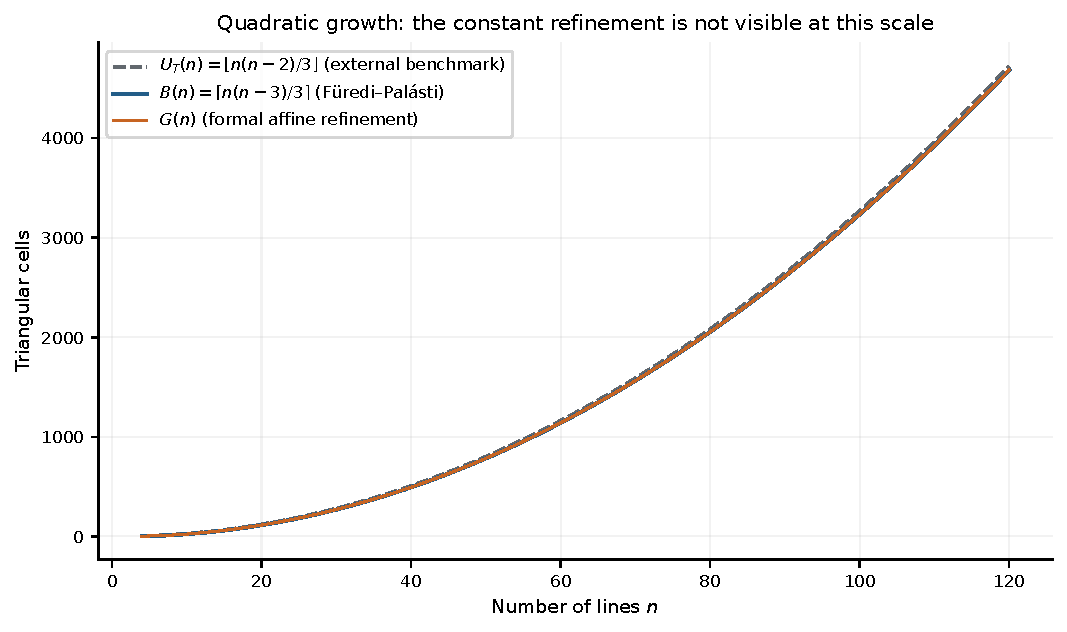
\includegraphics[width=0.94\linewidth]{bounds-growth.pdf}
\caption{Growth of the classical general baseline, the proved affine refinement, and the classical polynomial upper benchmark. The close overlap on a quadratic scale is mathematically meaningful: the new uniform gain is bounded. Residue and deficit plots below resolve the smaller differences. This figure is computed from the formulas, not copied from earlier publications.}\label{fig:growth}
\end{figure}

\subsection{Finite enhancements and other completed components}

The universal construction is supplemented by exact coordinates. Let $C(n)$ be the largest triangle count among the finite certificates in the release at order $n$, with $C(n)=0$ when no such certificate is saved. Then
\begin{equation}\label{eq:envelope}
\Lbound(n)=\max\{\G(n),C(n)\},\qquad \K(n)\ge\Lbound(n)
\end{equation}
is proved for all natural orders. This elementary maximum operation retains published constructions and the author's earlier values without altering their attribution. It is not a claim that $\Lbound$ is the largest lower bound obtainable from all published constructions by every possible interpolation or extension.

The finite catalog contains 138 distinct coordinate certificates, including 104 simple witnesses. A separate generated table has 64 orders at which a saved finite certificate strictly improves the older baseline $\B$; some of these improvements are already supplied by $\G$. The catalog includes weaker checkpoints and independent reproductions. Its size is not a count of original discoveries.

The October release adds a recursively closed geometric family. Put
$q_t=10\cdot2^t$ and $A_t=(q_t^2-4)/3$. For every $t\ge0$, simple
arrangements realize at least $A_t$ triangles at $q_t+1$ lines and
$A_t+q_t/2$ at $q_t+2$ lines. Every next seed retains the sorted grid,
saturation, positive central apex and visible-boundary data. Taking
the maximum of these candidates and $\Lbound$ gives the current total
bound $H$ of Theorem~\ref{fam:all-n-envelope}. It strictly improves
the previous repository envelope at every family pair from 321/322
onward, without claiming a new literature record for the inherited
numerical family.

Further completed components are actual exterior addition, its finite
boundary-resource obstruction, actual edge incidence and clean-line
charging, classical simple upper bounds and local fan restrictions.
The simple optimum at each recursive order is between the constructed
count and that count plus one. An explicit ten-sign obstruction on
the real 21-line tangent grid is also proved in Lean. Broader exact
classification checks and the uniform 49-line compatibility certificate
have separate evidence boundaries. Table~\ref{tab:claims} summarizes
the current release.

\begin{table}[tbp]
\centering\small
\begin{tabularx}{\linewidth}{@{}P{0.28\linewidth}XP{0.21\linewidth}@{}}
\toprule
Result & Mathematical content & Release status\\
\midrule
Universal $\G$ & Simple real-line witnesses at every order & General Lean proof\\
Envelope $\Lbound$ & Maximum with all saved finite witnesses & Lean; finite native checks\\
28:238, 30:275, 34:357 & Earlier attributed finite inequalities & Exact Lean certificates\\
Exterior extension & New line and gain from a visible-pair list & General Lean proof\\
Full successor recurrence & $\K(n+1)\ge\K(n)+\floor{n/2}$ & Unproved\\
49-seed numerical target & Lower function obtained by summing the proposed recurrence & Independently proved\\
One-step BBL doubling & $(q+1,T)\mapsto(2q+1,T+q^2)$ for compatible seeds & General Lean proof\\
Infinite hybrid iteration & Odd and full-gain even geometric families & Complete Lean; native seed\\
Local fan structure & Incidence, antipodal and run-length restrictions & General Lean proofs\\
Simple upper windows & Actual odd/even upper bounds and family existence & Complete Lean\\
Actual clean-line charging & Charge existence and finite fiber bounds & General Lean proof\\
Global multiplicity consequences & Core budgets requiring fan extraction & Conditional; bridge open\\
Tangent-grid obstruction & Explicit ten-sign algebraic impossibility & General Lean proof\\
\bottomrule
\end{tabularx}
\caption{Claim status in the 3 October mathematical release. ``General Lean proof'' does not imply that every proposed application has been formalized. Published construction inputs retain their original authorship.}\label{tab:claims}
\end{table}

\subsection{History, attribution, and the structure of the paper}

The March archive records a proposed extension from odd to even orders, associated finite bounds, and an incomplete Lean file. That file contains eight proof placeholders, including its central extension step. Later exact certificates establish the finite inequalities independently, while the current all-order proof uses a different construction. Accordingly, a corrected account must separate the survival of numerical conclusions from the validity of the original proof strategy.

The September work broadened the program to both parities, exterior visibility, boundary-defect estimates, compatible doubling seeds, exact rational realization, and multiplicity-sensitive upper arguments. Several plausible routes failed: direct repetition of exterior gains lost the necessary boundary resources; small perturbations of nonsimple records sometimes reduced the triangle count; and large local searches failed to improve their chosen seeds. These negative findings are recorded with their exact scope rather than converted into impossibility theorems. The October work closes the recursive and clean-line interfaces, adds rigorous grid obstructions, and leaves the unrestricted successor claim and global nonsimple fan extraction open.

Section~\ref{sec:geometry} states the geometric definitions and the certificate-to-cell bridge. Section~\ref{sec:universal} proves the uniform refinement; Section~\ref{sec:finite} records finite cases and provenance. The following sections develop extension and family results, local upper-bound ingredients, and computational searches. The final sections describe the formal trust boundary and future obligations. The appendices contain the complete finite tables and a map from mathematical claims to proof sources. The code and evidence are available at \repo~\cite{zarzueloRepository}.

\section{Literature, provenance, and the scope of comparison}
\label{lit:review}

\subsection{Four distinctions that affect every comparison}

The literature studies several related extremal functions. Their numerical tables cannot be combined without retaining their hypotheses. Throughout this paper, $\K(n)$ concerns straight lines in the real affine plane and permits multiple intersections and parallel pairs, whereas $\Ks(n)$ restricts to pairwise nonparallel lines with no three concurrent. Only bounded triangular cells are counted. A pseudoline arrangement is a topological relaxation; a lower bound obtained there becomes a straight-line lower bound only after realizability has been established. Finally, projective triangular faces need not remain bounded after an affine chart is chosen.

\begin{table}[htbp]
\centering\small
\begin{tabularx}{\textwidth}{@{}lXX@{}}
\toprule
Distinction & What transfers immediately & What requires another argument\\
\midrule
Simple / unrestricted & A simple example is an unrestricted example. & A simple upper bound need not bound a configuration with concurrent lines.\\
Straight / pseudoline & Every straight arrangement is a pseudoline arrangement. & A pseudoline construction requires a straight realization.\\
Affine / projective & Projective transformations preserve incidence and projective faces. & Boundedness depends on the line chosen as infinity.\\
Finite / infinite & A certified configuration proves its individual lower bound. & Iteration requires the next configuration to satisfy every input invariant.\\
\bottomrule
\end{tabularx}
\caption{Logical distinctions used throughout the source audit.}
\label{lit:scope-table}
\end{table}

There are also two different projective-to-affine operations. Choosing a new line at infinity outside an $n$-line arrangement keeps $n$ lines, but may lose triangular faces to infinity. Making one of the arrangement's own lines the line at infinity and removing it produces an $(n-1)$-line affine arrangement. The latter operation underlies several optimal subsequences; the former is central to the uniform construction formalized here.

\subsection{From the puzzle to arrangement theory}

Fujimura's puzzle reached English readers through \emph{The Tokyo Puzzles}, edited by Gardner and translated by Adachi~\citep{fujimura1978}; Gardner also discussed it in his collected mathematical recreations~\citep{gardner1983}. The broader theory of line and pseudoline arrangements is developed in Gr\"unbaum's monograph~\citep{grunbaum1972}. The papers of Strommer and Purdy document an established extremal-triangle literature preceding the construction used in this paper~\citep{strommer1977,purdy1979,purdy1980}. We cite those early papers as historical context rather than silently identifying all their projective or non-simple questions with the affine function $\K$.

The familiar comparison polynomial is
\begin{equation}
 U_{\mathrm T}(n)=\left\lfloor\frac{n(n-2)}3\right\rfloor.
 \label{lit:tamura}
\end{equation}
The attribution to Saburo Tamura is transmitted in the Cl\'ement--Bader draft~\citep{clementbader2007}; an original publication by Tamura was not located in this audit. We therefore do not manufacture an independent bibliographic item for that attribution. Cl\'ement and Bader report the stronger classical envelope $U_{\mathrm T}(n)-1$ for $n\equiv0,2\pmod6$. Section~\ref{upper:scope} explains both the scope of this reported result and a local proof-reading issue. A source-reported upper bound and an upper bound proved in our Lean development are different kinds of evidence.

\subsection{The F\"uredi--Pal\'asti all-order construction}

F\"uredi and Pal\'asti gave highly triangular straight-line arrangements using trigonometric coordinates~\citep{furedipalasti1984}. Their projective Table~1 has a residue-dependent constant term. The familiar affine consequence is commonly written
\begin{equation}
 \B(n)=\left\lceil\frac{n(n-3)}3\right\rceil\qquad(n\ge3).
 \label{lit:baseline}
\end{equation}
Erickson states this formula explicitly in Section~7.2 while using arrangements in a computational-geometric lower-bound argument~\citep{erickson1999}. Felsner and Kriegel place the construction in the study of Euclidean triangular cells~\citep{felsnerkriegel1999}. A later discussion by Dam\'asdi, Mart\'inez-Sandoval, Nagy and Nagy quotes the slightly weaker floor version while studying triangle areas~\citep{damasdi2020}. Thus a general lower bound valid at every order existed well before the present work.

Our completed formula is
\begin{equation}
 \G(n)=\left\lfloor\frac{n(n-3)}3\right\rfloor+1+(n\bmod2),
 \qquad n\ge4.
 \label{lit:our-formula}
\end{equation}
The constructions in later sections prove this for actual simple affine lines. Table~\ref{lit:residue-comparison} separates its arithmetic improvement over~\eqref{lit:baseline} from the projective count in the original paper. Here $P_{\mathrm{FP}}(n)$ denotes the latter construction's projective count, not the projective maximum.

\begin{table}[htbp]
\centering\small
\begin{tabular}{@{}cclc@{}}
\toprule
$n\bmod6$ & $\G-\B$ & $P_{\mathrm{FP}}(n)$, $n\ge5$ & $P_{\mathrm{FP}}-\G$\\
\midrule
0 & 1 & $n(n-3)/3$ & $-1$\\
1 & 1 & $(n^2-3n+5)/3$ & $0$\\
2 & 0 & $(n^2-3n+8)/3$ & $2$\\
3 & 2 & $(n^2-3n+9)/3$ & $1$\\
4 & 0 & $(n^2-3n+8)/3$ & $2$\\
5 & 1 & $(n^2-3n+5)/3$ & $0$\\
\bottomrule
\end{tabular}
\caption{Exact comparison with the quoted affine baseline and with the original projective construction's face counts. A projective surplus does not itself supply additional bounded affine triangles.}
\label{lit:residue-comparison}
\end{table}

The numerical gain is bounded by two. In particular, the quadratic coefficient $1/3$ and linear coefficient $-1$ remain unchanged. What the completed proof adds is a phase refinement, a controlled choice of affine chart for odd orders, and an end-to-end geometric formalization. The audited sources do not provide an explicit statement of~\eqref{lit:our-formula} with this affine proof. That observation is not an exhaustive numerical-priority theorem: old projective constructions contain related counts, and an unnoticed affine-chart argument could have been available earlier. The defensible claim is the proved improvement over the explicitly quoted formula~\eqref{lit:baseline}, together with the formal construction; a claim of first numerical discovery is withheld.

\subsection{Optimal subsequences and the straightening problem}

Harborth and Roudneff developed constructions and extremal results for pseudolines~\citep{harborth1985,roudneff1996}. Their scope matters because topological realizability does not imply straight realizability. Forge and Ram\'irez Alfons\'in constructed a projective straight-line family at orders $2\cdot2^t+2$\citep{forge1998}. Removing a distinguished line at infinity gives optimal affine orders $2\cdot2^t+1$; in particular, this is the relevant older source for the $33$-line order.

Bartholdi, Blanc and Loisel's preprint appeared in 2007 and its proceedings publication in 2008~\citep{bbl2008}. Their compatible doubling step takes $q+1$ lines to $2q+1$ and adds $q^2$ triangles. It requires a prescribed tangent grid and a fully used distinguished line. Their straight-line optimal series include $14\cdot2^t+1$ and $6\cdot2^t+1$; their $18\cdot2^t+1$ series was then a pseudoline result. The general numerical recurrence is therefore prior work, not a new theorem of this project. Our contribution is the verified real-coordinate specialization, a closed recursive seed invariant and its boundary-visibility refinement. The actual odd and adjacent-even induction is complete in this release; it does not transfer authorship of the published doubling gain.

Parpalak and Utkin supplied a compatible straight $19$-line seed and established the straight-line series $n=18\cdot2^t+1$\citep{parpalakutkin2026}. Its triangle count is $108\cdot4^t-1$. Substitution into our formula gives the exact comparison
\begin{equation}
 \bigl(108\cdot4^t-1\bigr)-\G(18\cdot2^t+1)=6\cdot2^t-2.
 \label{lit:pu-gap}
\end{equation}
Thus their series is stronger at these orders: the comparisons begin $107>103$ at $19$, $431>421$ at $37$, and $1727>1705$ at $73$. Their separate even-series draft is also relevant prior construction evidence~\citep{parpalakutkinEven2026}. Its numerical families are not replaced by a weaker universal formula.

It would consequently be misleading to call $\G$ the strongest numerical lower bound for every $n$, or an unqualified state of the art among all possible all-order formulas. Taking a maximum with known special constructions already improves it. Padding a configuration by lines sufficiently far away preserves its bounded triangles and extends each special construction to later orders. The retained function in the repository likewise takes a maximum with its finite certificate catalogue. The purpose of $\G$ is a compact uniform guarantee with a complete formal proof, not the suppression of stronger special cases.

\subsection{Upper-bound refinements retain their simplicity assumptions}

The even-order bound
\[
 \left\lfloor\frac{n(n-7/3)}3\right\rfloor
\]
in Bartholdi--Blanc--Loisel applies to \emph{simple affine pseudoline} arrangements. Blanc subsequently proved the sharper common even-order polynomial
\begin{equation}
 \Ks(n)\le\left\lfloor\frac{n(n-5/2)}3\right\rfloor,
 \qquad n\text{ even},
 \label{lit:blanc-even}
\end{equation}
also in the simple pseudoline setting~\citep{blanc2011}. The latter work was posted in 2008 and published in 2011. Its parity argument is the starting point for our clean-line accounting outside a multiple-point core.

The distinction is concrete. Formula~\eqref{lit:blanc-even} equals $53$ at $n=14$, whereas a nonsimple configuration with $54$ triangles exists. Applying a simple upper theorem to that configuration would be invalid. Our upper-bound work therefore counts shared sides and multiple incidences explicitly rather than treating a small perturbation to general position as automatically harmless.

\subsection{Recent computational constructions and versioned claims}

Savchuk's 2025 work combines arrangement tables, SAT search, and heuristic straightening~\citep{savchuk2025}. It reports optimal $23$- and $27$-line configurations and an exclusion of a perfect $33$-triangle arrangement at order $11$. Its Appendix~A.4 records the earlier Honma-based $11$-line construction. For our purposes, an arrangement table, a floating-point fit, an exact straight-line certificate, and an exhaustive upper-bound exclusion are four different outputs. The present work independently verifies the coordinate lower bounds it imports; it does not thereby replay the external SAT exclusions.

Maiorana released fifteen exact $14$-line, $54$-triangle configurations~\citep{maiorana2026}. We preserve their attribution and the source's CC BY 4.0 license. The current Parpalak--Utkin gallery supplies further exact constructions, including nonsimple even-order examples~\citep{parpalakutkinGallery2026}. The $8$-line construction has earlier provenance; citing its current host does not transfer its invention to the host authors. Each retained dataset is tied to a source revision, checked independently, and distinguished from any stronger optimality language used in its original repository.

Versioning also matters for exclusions. The fourth version of Liang, Liu and Zhang's preprint concerns symmetry restrictions for simple $28$-line configurations~\citep{liangliuZhang2026}. It is not treated here as a proof of an unrestricted exact value, and its displayed numerical comparison is not substituted for Blanc's simple upper theorem. The ProofAtlas research page similarly reports restricted upper results while keeping the unrestricted problem open~\citep{proofatlas2026}. We record these as current research sources, not as independently reproduced proofs.

\subsection{The 2026 enumeration and its use as external input}

Parpalak and Utkin's July 2026 preprint gives a reduced-word enumeration
and classification of triangle-maximal pseudoline arrangements, with
Euclidean and projective equivalence kept distinct
\cite{parpalakutkinEnumeration2026}. Its larger first-hit examples are
pseudoline constructions; straight realizability is a separate problem.
The present tangent-grid obstruction uses their supplied 21-line
classification as an external completeness input. Our exact replay
checks the algebraic contradiction certificates and all supplied
affine-class/support cases, not their full enumeration algorithm inside
Lean. Keeping the infinity support and every Euclidean class is
essential: a smaller list of projective representatives did not suffice
for the affine exclusion.

The compatible 49-line branch also requires careful comparison. Its
prospective odd family at $n=48\cdot2^t+1$ is the tail of BBL's older
$n=6\cdot2^s+1$ series, with $s=t+3$. The counts cannot be presented as
new lower-bound records. The uniform explicit slopes, whole-interval
sign certificate, boundary data and formal seed interface are the
contributions under investigation.

\subsection{The March result, later verification, and attribution}

The author's March manuscript proposed an even-order extension and recorded the values $238$, $275$, and $357$ at orders $28$, $30$, and $34$\citep{zarzuelo2026}. These values are now supported in this project by exact simple-line certificates. The associated original Lean file, however, contained placeholders, including the general extension lemma. The later successful formalizations do not retroactively turn that unfinished universal argument into a proof.

OEIS A006066 indexes numerical data, references, and named contributions~\citep{oeisA006066}. It is not a complete priority database. In particular, the 2007 Bartholdi--Blanc--Loisel table already contains a bold, hence straight-realizable, $30{:}275$ entry. The $34{:}357$ value follows from the older perfect $33$-line family and its exterior extension. At $28$ lines, Savchuk describes the analogous extension of the $27$-line solution. These overlaps require a distinction between an independently supplied construction, a new exact or formal certificate, and the first known numerical lower bound. We retain the author's recorded contribution without claiming first numerical priority solely from the OEIS attribution.

The recurrence reproduced by HandWiki~\citep{handwiki2026} is likewise a record of the proposed claim rather than a substitute for its proof. The unrestricted statement
\[
 \K(n+1)\ge\K(n)+\left\lfloor n/2\right\rfloor
\]
has not been established by the work reported here. What has been established includes a geometric exterior extension under explicit visibility hypotheses, finite successful successor steps, and a separate unconditional all-order construction. Their logical roles remain distinct.

\subsection{What formal verification contributes}

The proof infrastructure uses Lean~4~\citep{lean4} and mathlib~\citep{mathlib}. For the universal result, it connects analytic line equations, determinant signs, triangular cells, affine-chart control, and finite counting, rather than checking the final arithmetic formula in isolation. For finite results, it turns attributed coordinates into explicit certificates. For the upper-bound investigation, it now proves actual segment incidence, clean-line charging and the classical simple polynomial bounds, as well as local geometric restrictions. Extraction and summation of cyclic fans across a nonsimple core remain unfinished.

The accompanying repository~\citep{zarzueloRepository} records source revisions, negative searches, axiom reports, and the boundary between proved statements and proposed research. This separation is part of the result: a complete formal proof of a modest uniform improvement is stronger evidence than an ambitious recurrence with an unproved geometric step. It does not by itself confer numerical priority or solve the unrestricted Kobon problem.

\section{Real-line geometry and exact certificates}\label{sec:geometry}

\subsection{The two extremal problems}
\begin{definition}
An affine line is a set $\{(x,y)\in\R^2:ax+by=c\}$ with $(a,b)\ne(0,0)$. An arrangement is a finite set of distinct lines. A triangular cell is a bounded connected component of the complement whose closure is a nondegenerate triangle. The maximum number of such cells among arrangements of $n$ lines is $\K(n)$. The maximum among simple arrangements, with neither parallel lines nor triple concurrence, is $\Ks(n)$.
\end{definition}

The classical problem permits degeneracies that the simple problem excludes. Consequently $\Ks(n)\le\K(n)$, and a simple lower-bound construction is valid for both problems. The reverse use of an upper bound is invalid without a separate reduction. Our coordinate validator permits several lines through a triangular vertex, but excludes every line that cuts the triangle's interior.

The formal lower-bound predicate uses witnesses with no parallel pairs. This is a sufficient class of witnesses, not a claim that every maximizer of the classical problem has that property. For nontrivial orders, pairwise nonzero determinants also imply that every line is valid and that no two supporting lines coincide. The cases with fewer than three lines are handled separately.

\subsection{A polynomial sign certificate}

Represent a line $\ell$ by $(a_\ell,b_\ell,c_\ell)$, with affine evaluation $f_\ell(x,y)=a_\ell x+b_\ell y-c_\ell$. For two lines set
\begin{align}
D(\ell,m)&=a_\ell b_m-b_\ell a_m,\label{eq:det}\\
V(\ell,m)&=(X_{\ell m},Y_{\ell m},D(\ell,m))\\
&=(c_\ell b_m-b_\ell c_m,\ a_\ell c_m-c_\ell a_m,\ D(\ell,m)).\notag
\end{align}
When $D(\ell,m)\ne0$, their actual affine intersection is
$p_{\ell m}=(X_{\ell m}/D(\ell,m),Y_{\ell m}/D(\ell,m))$. For a third line $r$ define
\begin{align}
E(r;\ell,m)&=a_rX_{\ell m}+b_rY_{\ell m}-c_rD(\ell,m),\\
O(r;\ell,m)&=E(r;\ell,m)D(\ell,m).
\end{align}
The useful identity is
\begin{equation}\label{eq:oriented-affine}
O(r;\ell,m)=f_r(p_{\ell m})D(\ell,m)^2.
\end{equation}
Thus $O$ has the sign of the affine evaluation without requiring division in the certificate. All operations are polynomial over integer or rational coordinates.

\begin{definition}[Certified supporting triple]\label{def:certificate}
For a pairwise nonparallel arrangement $(\ell_0,\ldots,\ell_{n-1})$, an increasing triple $i<j<k<n$ is certified if
\begin{enumerate}
\item $E(\ell_k;\ell_i,\ell_j)\ne0$;
\item for each line $r$ of the arrangement, the three numbers
\[
O(r;\ell_i,\ell_j),\quad O(r;\ell_i,\ell_k),\quad O(r;\ell_j,\ell_k)
\]
are either all nonnegative or all nonpositive.
\end{enumerate}
The first condition excludes concurrence of the three supports; the second permits zeros at vertices but forbids a strict sign change.
\end{definition}

\begin{theorem}[From a sign certificate to a triangular cell]\label{thm:certificate-cell}
Every certified supporting triple determines a nondegenerate bounded triangular cell. Its interior is nonempty. Two distinct increasing certified triples determine disjoint interiors.
\end{theorem}
\begin{proof}
The three pair intersections exist because their denominators in~\eqref{eq:det} are nonzero. The nonvanishing evaluation excludes concurrence and gives three noncollinear points. Their positive barycentric combinations form a nonempty open triangle $\Delta$.

By~\eqref{eq:oriented-affine}, each arrangement line has a common weak sign at the three vertices. Affine linearity gives the same sign throughout the closed triangle. It is strict in $\Delta$: otherwise all three vertex evaluations would be zero, forcing a valid line to contain three noncollinear points. Hence no arrangement line enters $\Delta$.

Fix an interior point $z$. Its strict sign cell is
\[
S_z=\{x\in\R^2:f_r(x)f_r(z)>0\text{ for every arrangement line }r\}.
\]
The preceding argument gives $\Delta\subseteq S_z$. Conversely, the three support inequalities alone force all three barycentric coordinates of $x$ to be positive, so $S_z\subseteq\Delta$. The sign cell is an intersection of open half-planes and is convex; it is exactly a component of the complement. It is bounded by the three finite segments of the triangle.

If two certified interiors meet, they have the same strict sign vector and hence the same sign cell. Its three supporting lines are determined by its three open sides. Since distinct arrangement lines cannot share an open side, the sets of supports agree, and sorting their indices makes the triples equal. The contrapositive proves disjointness.
\end{proof}

The modules \lean{Kobon.Euclidean} and \lean{Kobon.Cells} prove the sign-cell and nonoverlap content through \lean{interior_nonempty}, \lean{interior_eq_signCell}, and \lean{distinct_interiors_disjoint}. The connected-component interpretation is the elementary convexity argument above; it is not separately encoded through a topological component API. Thus the certificates have an explicit interpretation as actual Kobon cells.

\subsection{What a finite lower-bound certificate establishes}

\begin{proposition}[Soundness of exact finite validation]\label{prop:finite-sound}
Let $A$ be an array of $n$ integer line coefficients, and let $\mathcal T$ be a list of at least $T$ certified increasing triples with no duplicates. If all pair determinants are nonzero, then $\K(n)\ge T$. If all increasing triples of lines additionally have nonzero concurrence determinant, then $\Ks(n)\ge T$.
\end{proposition}
\begin{proof}
The coefficient inclusion $\Z\hookrightarrow\R$ preserves polynomial equalities, strict inequalities, and weak signs. The resulting real arrangement therefore satisfies Definition~\ref{def:certificate}. Apply Theorem~\ref{thm:certificate-cell} to the distinct triples. The additional concurrence test is exactly the simplicity condition.
\end{proof}

Rational coordinates are cleared of denominators line by line before the integer check. The mathematical lower bound needs only a list of $T$ valid triangles; it need not prove that no further triangle exists in the same arrangement. For the catalog, however, two independent exact counters also enumerate the triangle count. One works from consecutive intersections along each line, while the other directly tests triples against the arrangement. Agreement is an independent check on extraction and counting, not a substitute for the general soundness theorem.

These distinctions explain the three evidential levels used later. A proved symbolic theorem applies at arbitrary order. A finite Lean certificate establishes its listed order. An exact experimental count outside the catalog remains a computationally verified witness until promoted through the same formal pipeline. No finite list, however large, proves an infinite family.

\section{A parity-sensitive all-order construction}\label{sec:universal}

This section gives the mathematical ingredients of Theorem~\ref{thm:main}. The underlying trigonometric family is a version of the classical F\"uredi--Pal\'asti family. Its attribution is independent of the present formalization and choice of affine chart.

\subsection{Trigonometric geometry and the classical count}

For $0<\theta<\pi$, define
\begin{equation}\label{eq:trig-line}
\ell(\theta):\quad \sin\theta\,x+\cos\theta\,y=\sin(3\theta).
\end{equation}
The normal has length one. Direct trigonometric expansion gives
\begin{align}
D(\ell(x),\ell(y))&=\sin(x-y),\label{eq:trig-det}\\
E(\ell(z);\ell(x),\ell(y))
&=4\sin(x-y)\sin(z-y)\sin(z-x)\sin(x+y+z).\label{eq:trig-eval}
\end{align}
In particular, distinct angles in $(0,\pi)$ give nonparallel lines. Multiplying~\eqref{eq:trig-eval} by~\eqref{eq:trig-det} yields
\begin{equation}\label{eq:trig-oriented}
O(\ell(z);\ell(x),\ell(y))=
4\sin^2(x-y)\sin(z-y)\sin(z-x)\sin(x+y+z).
\end{equation}
Only three factors determine the sign on the right.

For the half-phase choice $\theta_i=(i+1/2)\pi/n$, select increasing triples with
\begin{equation}\label{eq:halfphase-triples}
i+j+k\equiv n-1\ \text{or}\ n-2\pmod n.
\end{equation}
For the shifted choice $\theta_i=(i+1/6)\pi/n$, select instead
\begin{equation}\label{eq:shifted-triples}
i+j+k\equiv0\ \text{or}\ n-1\pmod n.
\end{equation}

\begin{lemma}[Triangle selection]\label{lem:trig-triangles}
For $n\ge3$, the triples in~\eqref{eq:halfphase-triples} certify triangles of the half-phase arrangement. The triples in~\eqref{eq:shifted-triples} certify triangles of the shifted arrangement. Both arrangements are simple.
\end{lemma}
\begin{proof}[Sign proof]
The angle sum of any three lines is $(i+j+k+3/2)\pi/n$ in the first arrangement and $(i+j+k+1/2)\pi/n$ in the second. It is never an integer multiple of $\pi$, which, together with~\eqref{eq:trig-eval}, excludes triple concurrence.

For a selected $i<j<k$, fix a fourth index $r$. The factors $\sin(\theta_r-\theta_j)$ and $\sin(\theta_r-\theta_i)$ change sign only when $r$ passes the corresponding support index. For each of the pairs $(i,j),(i,k),(j,k)$, the remaining factor is
$\sin((i+j+r+3a)\pi/n)$ with $a=1/2$ or $1/6$. Substituting the selected residue of $i+j+k$ fixes on which side of the next multiple of $\pi$ this sum lies when $r<k$ and when $r>k$. Splitting the index range at $i,j,k$ shows that the three expressions in~\eqref{eq:trig-oriented} have one weak sign in each range. At a support index the appropriate evaluations are zero. Their common sign need not be the same for different $r$; that is precisely the permitted sign choice in Definition~\ref{def:certificate}.

Equivalently, this check uses only the sign of $\sin t$ on consecutive intervals $(s\pi,(s+1)\pi)$ and the inequalities $0\le r<n$. No numerical trigonometric approximation is used. The complete index splits are proved in \lean{FurediPalasti.lean} and \lean{ShiftedFurediPalasti.lean}. Definition~\ref{def:certificate} and Theorem~\ref{thm:certificate-cell} then give the claimed cells.
\end{proof}

For any residue $b\in\Z/n\Z$, the equation $i+j+k=b$ has exactly $n^2$ ordered solutions. At most $3n$ have a repeated index, because each of $i=j$, $j=k$ and $i=k$ leaves at most $n$ choices. Two distinct residue classes therefore give at least $2n^2-6n$ ordered distinct-index triples. Each increasing triple accounts for six permutations, so the half-phase arrangement has at least
\begin{equation}\label{eq:classical-count}
\ceil{\frac{2n^2-6n}{6}}=\B(n)
\end{equation}
certified triangles. This is the classical all-order estimate, now proved directly in the real-coordinate formalization.

\subsection{The repeated-index correction}

\begin{lemma}[Shifted count]\label{lem:shifted-count}
For every $n\ge3$, the shifted arrangement has at least
\[
\floor{\frac{n(n-3)}3}+1
\]
certified triangular cells.
\end{lemma}
\begin{proof}
Use the two residues $0$ and $n-1$ in~\eqref{eq:shifted-triples}. In the zero residue, the three repeated-index sets all contain $(0,0,0)$. Their union therefore has at most $3n-2$ members, not merely $3n$. In the other residue retain the bound $3n$. The number of ordered distinct-index solutions is at least $2n^2-6n+2$. If $T$ is the number of increasing selected triples, then
\[
6T\ge2n^2-6n+2,
\qquad
T\ge\ceil{\frac{n(n-3)+1}{3}}
=\floor{\frac{n(n-3)}3}+1.
\]
Lemma~\ref{lem:trig-triangles} supplies their actual geometry. This argument uses the overlap of bad-index sets, not a numerical rounding conjecture.
\end{proof}

\begin{figure}[tbp]
\centering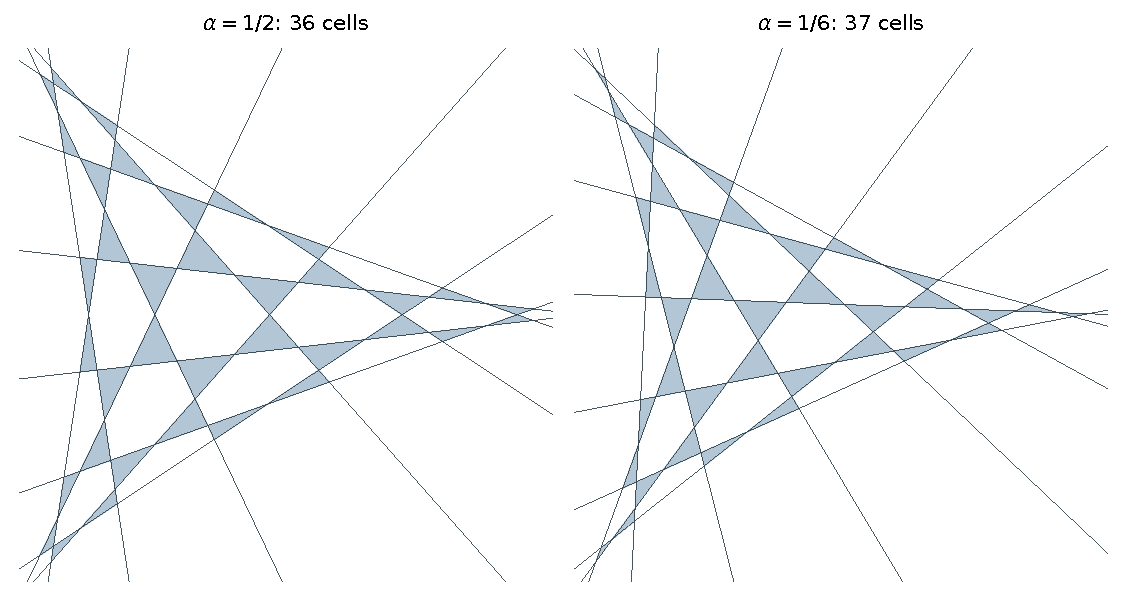
\includegraphics[width=0.9\linewidth]{phase-family.pdf}
\caption{New rational-coordinate illustrations at $n=12$, obtained from the half-phase and shifted trigonometric families. Two independent exact counters certify 36 and 37 triangles in these rational proxies. The axes of each panel are rescaled independently. The real-coordinate universal theorem follows from the symbolic sign and modular arguments, independently of this illustration. The underlying family is attributed to F\"uredi and Pal\'asti.}\label{fig:phase}
\end{figure}

\subsection{Projective changes of affine chart}

The shifted count is enough for the even part of~\eqref{eq:G}. To obtain the additional odd-order gain we use exposed vertices of the half-phase arrangement. The exact coordinate map is
\begin{equation}\label{eq:projective-map}
(x,y)\longmapsto \left(\frac{x}{h-x},\frac{y}{h-x}\right),\qquad h\ne0.
\end{equation}
It replaces the line $x=h$ by the line at infinity. The transformed coefficients of $ax+by=c$ are
\begin{equation}\label{eq:line-transform}
\Phi_h(a,b,c)=(ha-c,hb,c).
\end{equation}
Unlike an affine transformation, this change can alter which projective triangular faces appear bounded. Thus counting triangles before and after the change requires an explicit sign argument.

\begin{lemma}[Exact covariance]\label{lem:projective-covariance}
If $D(\ell,m)\ne0$, then
\begin{align}
D(\Phi_h\ell,\Phi_hm)&=hD(\ell,m)(h-x_{\ell m}),\\
E(\Phi_hr;\Phi_h\ell,\Phi_hm)&=h^2E(r;\ell,m),\\
O(\Phi_hr;\Phi_h\ell,\Phi_hm)&=h^3(h-x_{\ell m})O(r;\ell,m),\label{eq:projective-sign}
\end{align}
where $x_{\ell m}$ is the abscissa of the old intersection. If the cut avoids every old vertex, the transformed arrangement has no parallel pairs. Triple nonconcurrence is preserved.
\end{lemma}
\begin{proof}
Substitute~\eqref{eq:line-transform} into the polynomial expressions in Section~\ref{sec:geometry}, expand, and cancel. Nonzero $h$ and avoidance of all $x_{\ell m}$ give the pair determinant claim, while multiplication by $h^2$ preserves a nonzero triple evaluation.
\end{proof}

The sign multiplier in~\eqref{eq:projective-sign} also gives a direct triangle-preservation rule. If $h>0$ and all vertices of a certified triangle lie to the left of $x=h$, all three multipliers are positive. If $h<0$ and its vertices lie to the right, they are again positive. At selected exposed vertices on the opposite side, the sign reverses. Carefully choosing which vertices are separated by the cut creates the extra triangles.

\begin{lemma}[One exposed vertex]\label{lem:one-cap}
For odd $n=2m+1\ge3$, a change of affine chart of the half-phase arrangement has at least $\B(n)+1$ bounded triangles.
\end{lemma}
\begin{proof}
The intersection of $\ell(x)$ and $\ell(y)$ has abscissa
\begin{equation}\label{eq:vertex-x}
X(x,y)=\cos(2x)+\cos(2y)+\cos(2x+2y).
\end{equation}
For the half-phase angles, the vertex of lines $0,n-1$ is uniquely rightmost, with abscissa $c_n=1+2\cos(\pi/n)>0$. Indeed, each of the first two cosine terms in~\eqref{eq:vertex-x} is at most $\cos(\pi/n)$ and the last is at most one; if the pair is not $(0,n-1)$, at least one necessary inequality is strict. Choose $h>0$ between all other abscissae and $c_n$.

No selected triangle of~\eqref{eq:halfphase-triples} uses the pair $(0,n-1)$: such a triple would require its middle index to be $0$ or $n-1$ modulo $n$. Hence all counted triangles are preserved by the positive multiplier rule. The additional triple $(0,m,2m)$ has, for each test line, nonnegative evaluation at the exposed vertex and nonpositive evaluations at its other two vertices before the transformation. The cut reverses exactly the exposed-vertex sign, so the transformed triple satisfies the certificate. These signs follow from~\eqref{eq:trig-oriented} by splitting the test index at $m$. The triple is absent from the old selected list, and Lemma~\ref{lem:projective-covariance} preserves simplicity. This gives one additional bounded triangle.
\end{proof}

\begin{lemma}[Two exposed vertices]\label{lem:two-caps}
For $n=6k+3$ with $k\ge1$, a change of affine chart of the half-phase arrangement has at least $\B(n)+2$ bounded triangles.
\end{lemma}
\begin{proof}
Write $n=3m$, where $m=2k+1$. The two intersections supported by $(m-1,m)$ and $(2m-1,2m)$ have common abscissa $-c_n/2$. Every other intersection has strictly larger abscissa. To verify the latter assertion, rewrite~\eqref{eq:vertex-x} as
\[
X(u,v)=2zw+2z^2-1,
\qquad z=\cos(u+v),\quad w=\cos(u-v).
\]
For nonadjacent angle indices, the cosine bounds on the discrete grid, together with completing the square in $z$, give $X>-c_n/2$. For adjacent indices, $w=\cos(\pi/n)$ and the same quadratic attains equality precisely at $u+v=2\pi/3$ or $4\pi/3$, giving the two listed pairs. The exceptional wrapping pair $(0,n-1)$ is the rightmost vertex. These exposure inequalities are proved uniformly in \lean{FurediPalastiCaps.lean}.

Choose $h<0$ strictly above $-c_n/2$ and below all other abscissae. The modular conditions~\eqref{eq:halfphase-triples} show that no counted triangle uses either exposed pair. Its vertices are therefore all to the right of the cut and its signs are preserved. The two additional support triples are
\[
(2k,2k+1,5k+2),\qquad (k,4k+1,4k+2).
\]
For each test index, substitution into~\eqref{eq:trig-oriented} gives one sign at the exposed pair and its opposite weak sign at the other two vertices. The negative cut reverses exactly the exposed-vertex multiplier in each case, establishing the transformed certificates. The two triples are distinct and neither satisfies the old selection residues. Simplicity follows from Lemma~\ref{lem:projective-covariance}. Appending both triples to the retained list proves the claim.
\end{proof}

\begin{figure}[tbp]
\centering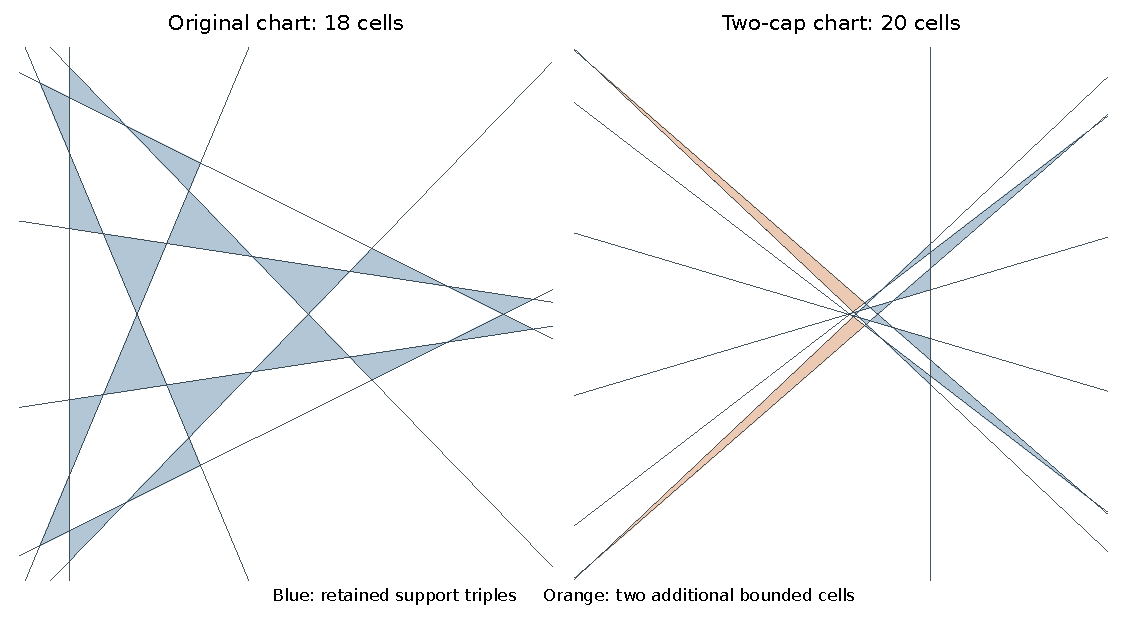
\includegraphics[width=0.95\linewidth]{affine-chart.pdf}
\caption{New exact rational illustration at $n=9$: the change of affine chart retains all 18 old triangular cells and creates two more. The resulting 20 is below the known optimum 21; this figure illustrates the uniform mechanism. Panels are rescaled independently. Both counts are checked exactly. The general proof tracks the determinant multiplier at every vertex, independently of the drawing.}\label{fig:chart}
\end{figure}

\subsection{Assembly, exact gain, and asymptotic scale}

\begin{proof}[Proof of Theorem~\ref{thm:main}]
Use Lemma~\ref{lem:shifted-count} for even $n\ge4$. For odd $n$ not divisible by three, $n(n-3)\equiv1\pmod3$, so
$\B(n)+1=\floor{n(n-3)/3}+2$; apply Lemma~\ref{lem:one-cap}. For odd multiples of three at least nine, $\B(n)=n(n-3)/3$ and Lemma~\ref{lem:two-caps} gives the same target. Three nonconcurrent lines give $\G(3)=1$, while the smaller cases have zero triangles. Each construction used is simple.
\end{proof}

\begin{corollary}[Exact improvement over the quoted baseline]\label{cor:gain}
For $n\ge4$,
\[
\G(n)-\B(n)=
\begin{cases}
1+(n\bmod2),&3\mid n,\\
n\bmod2,&3\nmid n.
\end{cases}
\]
The gains in classes $0,1,2,3,4,5\pmod6$ are respectively $1,1,0,2,0,1$.
\end{corollary}
\begin{proof}
The product $n(n-3)$ is zero modulo three when $3\mid n$, and one modulo three otherwise. Substitute these remainders in the floor and ceiling formulas.
\end{proof}

\begin{figure}[tbp]
\centering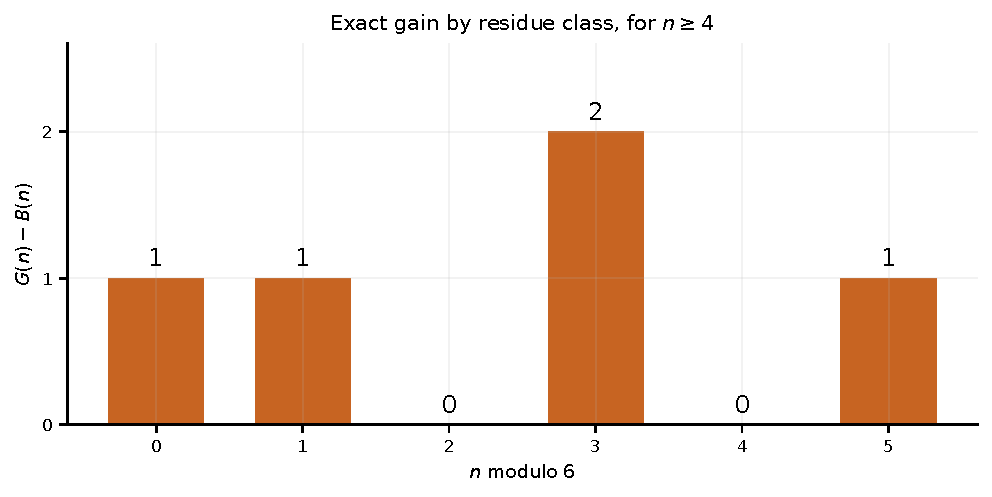
\includegraphics[width=0.88\linewidth]{residue-gains.pdf}
\caption{The exact proved gain $\G-\B$, resolved by residue class modulo six. The gain is strict on four classes; the universal statement includes arbitrarily large orders in each class.}\label{fig:residue}
\end{figure}

For comparison with the classical polynomial benchmark $\U(n)=\floor{n(n-2)/3}$, direct integer arithmetic gives, for $n\ge4$,
\begin{equation}\label{eq:gap}
\U(n)-\G(n)=\floor{\frac n3}+\mathbf1_{n\equiv2\ (3)}-1-(n\bmod2).
\end{equation}
This comparison is arithmetic. Section~\ref{upper:simple-actual} now formalizes the classical simple upper theorem; unrestricted attribution remains external. The deficit is still of order $n$, and sharper bounds or special constructions apply at some orders.

\begin{figure}[tbp]
\centering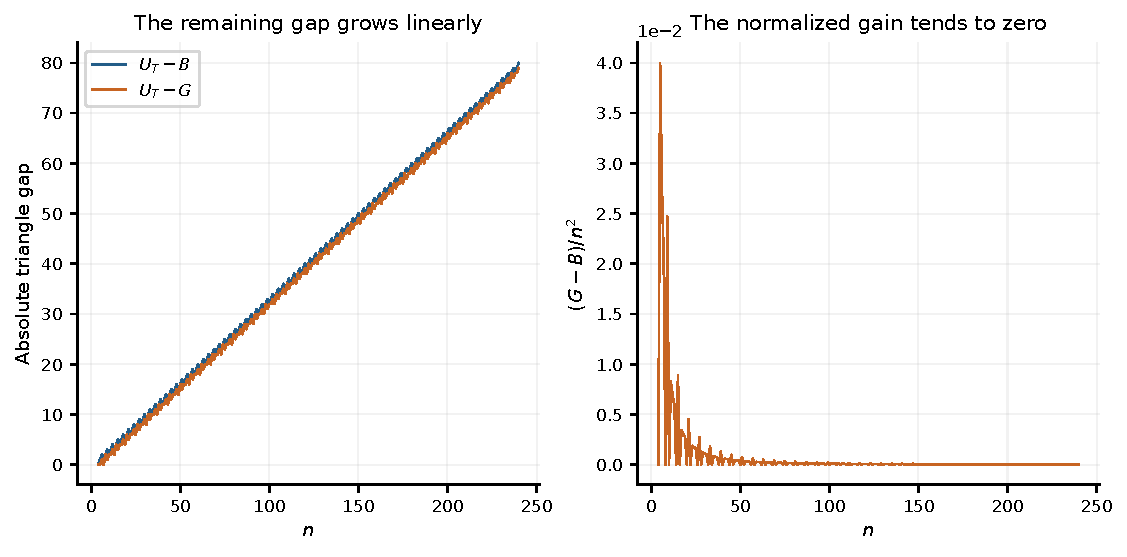
\includegraphics[width=0.94\linewidth]{normalized-gap.pdf}
\caption{Deficit and normalized growth computed from the proved formulas. The constant improvement is visible in the deficit, while both general lower formulas have the same leading quadratic and linear terms. The polynomial is the classical benchmark, now also formalized for simple arrangements; its numerical upper bound is not new.}\label{fig:normalized}
\end{figure}

The outcome is an unconditional affine theorem, stronger than the quoted baseline at infinitely many orders. Its numerical first priority remains a separate literature question. The construction gives a witness for each $n$; it does not provide an operation that adds one line to every preceding optimal witness.

\section{Individual cases, finite enhancements, and provenance}\label{sec:finite}

\subsection{The March values and their present verification}

The three finite inequalities associated with the author's early extension work are
\begin{equation}\label{eq:march-three}
\K(28)\ge238,\qquad \K(30)\ge275,\qquad \K(34)\ge357.
\end{equation}
Each now has an exact simple-arrangement certificate, so the same inequalities hold for $\Ks$. Their present validity is independent of the unproved recurrence in the original March manuscript. The certificates give actual lines and complete checked triangle lists, not only numerical consequences of an extension hypothesis.

The current OEIS table associates the name Zarzuelo with these entries~\cite{oeisA006066,zarzuelo2026}. Attribution in an index and first discovery are different questions. The earlier literature already contains matching constructions or consequences for some of these counts; the literature review records these overlaps. The claims made here are the documented attribution trail, the independently verified witnesses, and their place in the author's extension program. No new priority claim is inferred from the absence of a value from a particular online table.

\begin{figure}[tbp]
\centering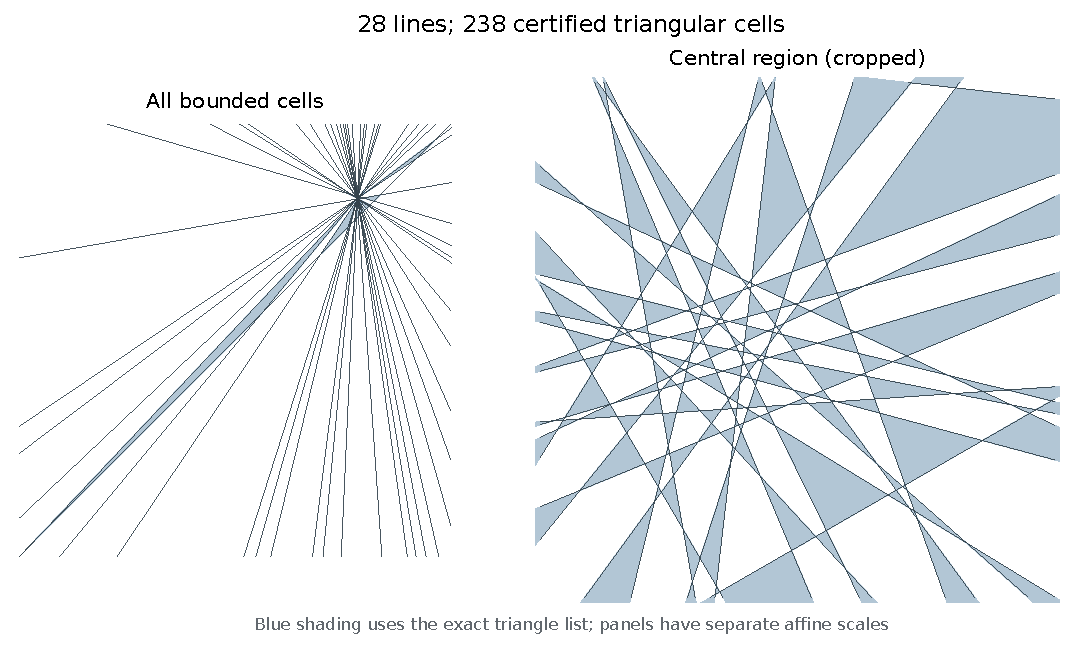
\includegraphics[width=0.96\linewidth]{historical-28.pdf}
\caption{The retained exact 28-line witness with 238 certified triangles. This is a new rendering of the saved coordinates associated with the earlier extension program. The marked zoom, where present, is an enlargement of the same arrangement; it does not add or remove lines from the certificate. The picture illustrates a lower bound, while the exact sign tests establish it.}\label{fig:historical28}
\end{figure}
\begin{figure}[tbp]
\centering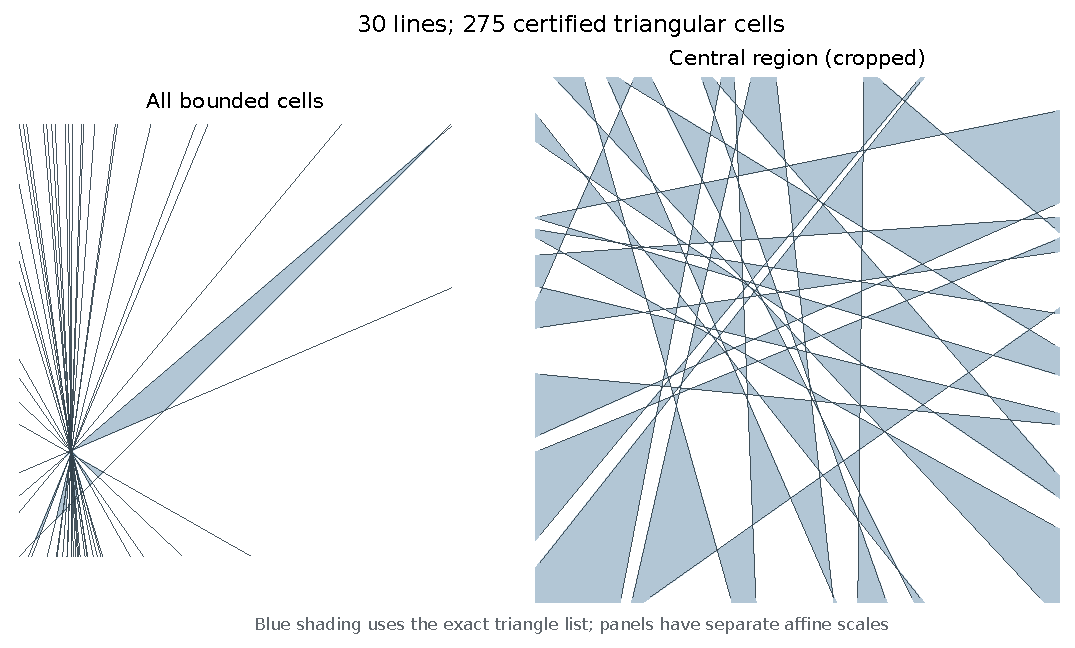
\includegraphics[width=0.96\linewidth]{historical-30.pdf}
\caption{The retained 30-line witness with 275 certified triangles, rendered from its exact coordinates. The count has prior literature overlap and is not asserted to be a new numerical record. The complete witness remains in the catalog even though the historical general extension proof was incomplete.}\label{fig:historical30}
\end{figure}
\begin{figure}[tbp]
\centering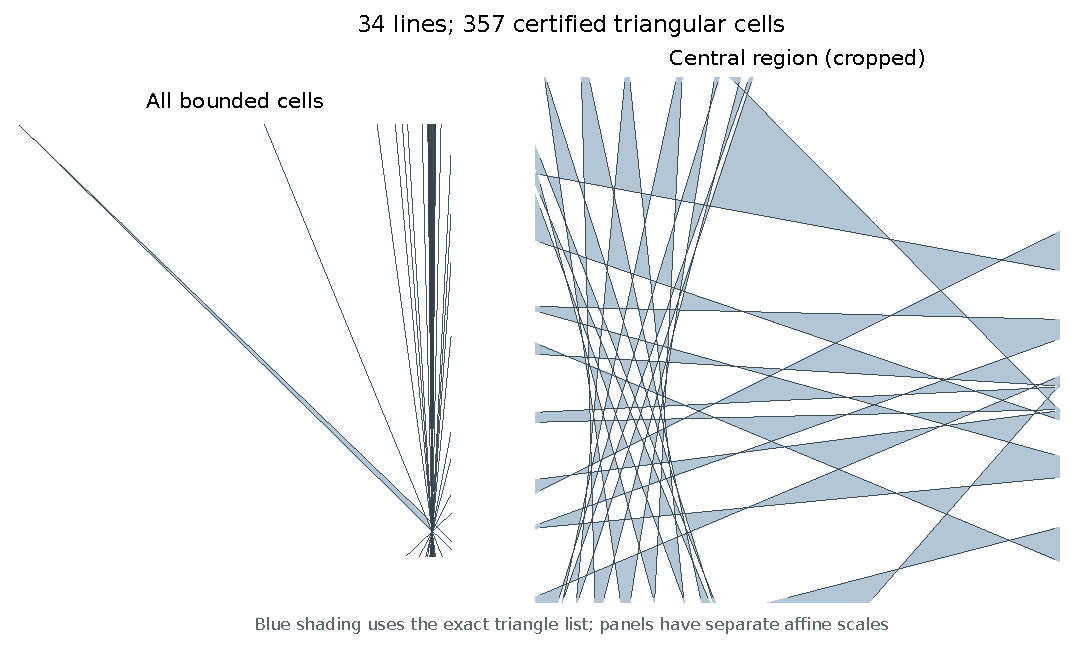
\includegraphics[width=0.96\linewidth]{historical-34.pdf}
\caption{The retained 34-line witness with 357 certified triangles. Original plotting of the certificate makes the finite conclusion inspectable independently of the claimed universal extension. The construction input and earlier matching literature are credited separately.}\label{fig:historical34}
\end{figure}

The original inventory also listed outputs for every order from 3 through 60, together with larger cases at 99 and 195. Some were direct certificates, some were numerical consequences of a boundary-defect argument, and many were weaker than an already available construction. Appendix~\ref{app:historical} preserves that inventory as history. The current certificate aliases independently retain its numerical inequalities; a label inherited from the old table is not used as a present formal-proof status.

\subsection{Materialized improvements from the phase and chart construction}

Table~\ref{tab:finite-refinement} records simple rational witnesses promoted during the last construction phase. Each listed new count is supplied by the universal theorem and also realized by an independently checked finite coordinate file. This double presentation is useful: the theorem proves all orders, while the coordinates support visualization and further exact searches.

\begin{table}[tbp]
\centering
\begin{tabular}{@{}rrrr@{}}
\toprule
$n$ & Earlier retained count & Current simple count & Increase\\
\midrule
39&469&470&1\\
47&690&691&1\\
48&720&721&1\\
51&817&818&1\\
53&884&885&1\\
54&918&919&1\\
55&954&955&1\\
59&1102&1103&1\\
60&1140&1141&1\\
99&3169&3170&1\\
195&12481&12482&1\\
\bottomrule
\end{tabular}
\caption{Changes relative to this project's previous retained witnesses, not a table of first discoveries or global record improvements. ``Simple'' is certified for every current coordinate witness in this table.}\label{tab:finite-refinement}
\end{table}

In particular, the earlier additional-line values $39:469$, $51:817$, $99:3169$ and $195:12481$ are now exceeded by $\G$ itself. Their finite correctness survives, but those numbers are not distinctive of the additional-line family. Historical evidence is retained rather than deleted when a stronger construction is found.

\subsection{The 44-line simple case}

The exact exterior extension of the retained 43-line arrangement creates 21 triangles while preserving its 587 old triangles. Both exact counters and the Lean certificate give a simple 44-line arrangement with 608 triangles. Blanc's classical simple upper bound at this order is also 608~\cite{blanc2011}. Both inequalities are now formally supported, giving
\begin{equation}\label{eq:44-simple}
\Ks(44)=608.
\end{equation}
The finite Lean certificate supplies the lower inequality, and
\sourcefile{Kobon/UpperEvenSimpleOptimality.lean}{\lean{UpperEvenSimpleOptimality}}
supplies the simple upper inequality. Equation~\eqref{eq:44-simple} is
their immediate numerical corollary, not a separate maximality wrapper.
It neither establishes $\K(44)=608$ for unrestricted arrangements nor
claims first discovery of this numerical value.

This example shows why upper-bound scope belongs next to the numerical statement. A simple witness can establish a classical lower bound, but a simple upper theorem cannot by itself close the classical problem.

\subsection{External records and independently checked inputs}

The updated catalog incorporates exact gallery witnesses from Parpalak and Utkin at
\[
8:15,\ 14:54,\ 20:117,\ 26:204,\ 32:315,\ 36:402,\ 38:450,\ 42:553,\ 46:667,\ 50:792.
\]
These are constructions or coordinate sources of the cited researchers, not newly discovered values in this project. The eight-line value has older priority; the modern gallery is the source of the checked coordinates. The public source snapshot and the formal certificate index preserve the provenance~\cite{parpalakutkin2026,oeisA006066}.

All fifteen of Maiorana's supplied 14-line arrangements with 54 triangles were independently checked and promoted as finite certificates~\cite{maiorana2026}. Fourteen have two triple points and one has four. Their source license and immutable commit are retained. These witnesses are a particularly useful warning against conflating simple and nonsimple arrangements: removing a multiple intersection by a small perturbation need not preserve the full triangle count. Section~\ref{exp:section} reports the exact resolution experiments.

The two source snapshots used for these imports are Maiorana commit
\nolinkurl{e47c7cfd9661e54d29befb83118bf83d5f804028} and gallery commit
\nolinkurl{feae4f5571a988a3ed45bd26a36259ebb7d7d3d2}. Their mathematical attribution is attached to each source record even when a new Lean wrapper or new figure is generated here.

\subsection{The finite envelope and the complete tables}

\begin{proposition}[Retained all-order envelope]\label{prop:envelope}
Let $C(n)$ be the maximum count in the finite catalog at order $n$, or zero if that order is absent. Then $\K(n)\ge\Lbound(n)=\max\{\G(n),C(n)\}$ for every $n$. In the frozen release, $\Lbound(n)=\G(n)$ for every $n>195$.
\end{proposition}
\begin{proof}
When $C(n)\le\G(n)$, use Theorem~\ref{thm:main}. Otherwise choose a certificate attaining the finite maximum and apply Proposition~\ref{prop:finite-sound}. No coordinate certificate in this release has order greater than 195. Larger computational witnesses discussed later have not been silently added to the Lean catalog.
\end{proof}

The formal definition is {\small\texttt{Universal.bound = max Universal.baseline AllN.bound}}. Since $\G\ge\B$, it equals the expression in Proposition~\ref{prop:envelope}; the older \lean{AllN} layer preserves the previous finite-envelope theorem. This makes comparisons reproducible without rewriting the historical construction history.

\begin{figure}[tbp]
\centering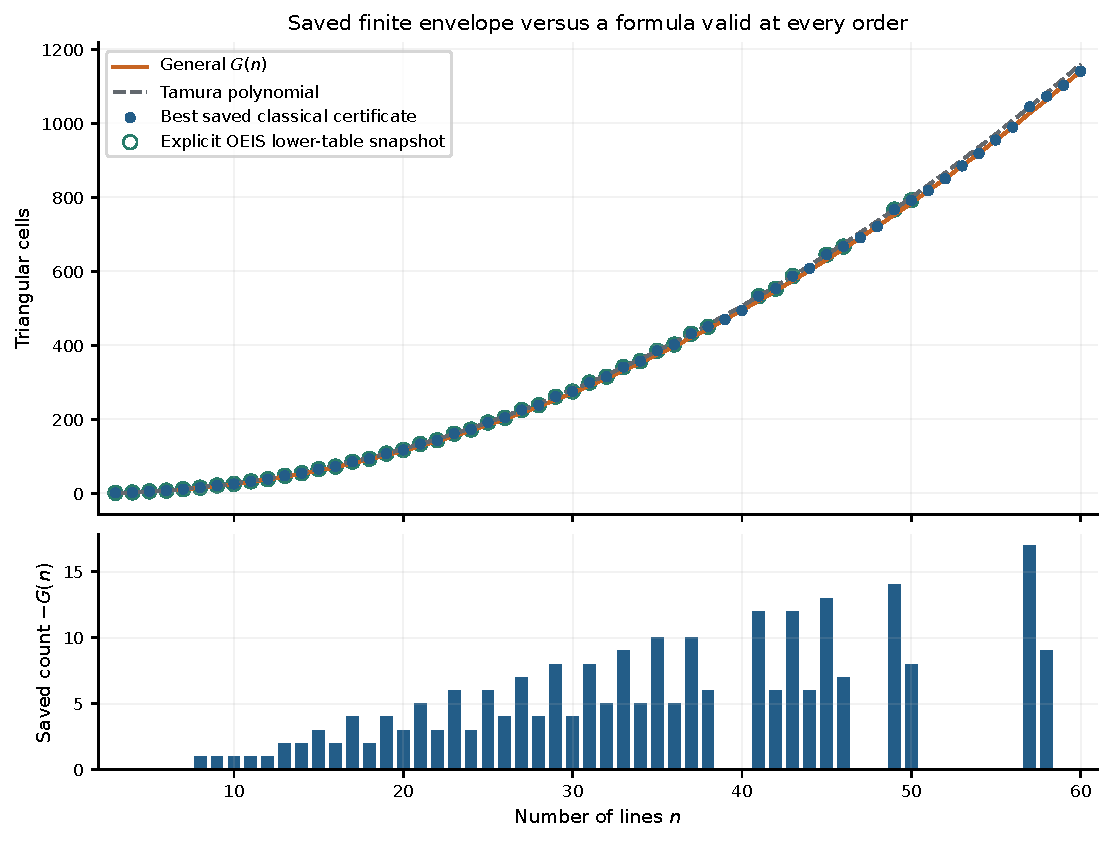
\includegraphics[width=0.96\linewidth]{finite-envelope.pdf}
\caption{The strongest saved simple and classical coordinate counts, compared with the uniform formula and the polynomial upper benchmark. External witnesses retain their attribution. A marker above $\G$ is a finite enhancement of the general formula, not automatically an original record.}\label{fig:finite-envelope}
\end{figure}

Appendix~\ref{app:finite-table} gives the best saved simple and classical values from 3 through 60. Appendix~\ref{app:catalog} lists all 138 certificate identities, including repeated orders and weaker checkpoints. Appendix~\ref{app:historical} gives the older author-output inventory. Together these tables prevent three common confusions: a retained output is not necessarily the best available value; a missing OEIS row is not proof of novelty; and an exact count for one arrangement is not automatically the extremal value $\K(n)$.

\section{Exterior extensions: the March proposal and its precise replacement}
\label{ext:section}

The starting point of this project was the March 2026 proposal that an odd
Kobon arrangement could always be extended with the gain
\begin{equation}
  \K(2m+2)\geq \K(2m+1)+m.
  \label{ext:march}
\end{equation}
The proposal was presented in \cite{zarzuelo2026} and subsequently described
as an iterative rule in \cite{handwiki2026}.  The preserved March source is
important evidence of the development of the idea, but is not a completed
proof of \eqref{ext:march}: its Lean file contains eight proof placeholders,
including the extension assertion.  The present work replaces the informal
alternating-segment argument by an actual geometric extension theorem and
identifies exactly which additional counting hypothesis yields the desired
gain.  Independently verified finite bounds are retained regardless of the
status of that original argument.

The later OEIS attribution at orders 28, 30, and 34 is evidence of the
proposal's reception, rather than a proof of numerical
priority~\cite{oeisA006066}.  In particular, the BBL table already records
the straight-line value $30:275$.  The perfect 33-line input belongs to
the family of Forge and Ram\'irez Alfons\'in~\cite{forge1998}; applying the
exterior extension stated by BBL gives $34:357$~\cite{bbl2008}.
The historical attribution, the validity of a finite count, and the
novelty of a general extension theorem are therefore assessed separately.

Two distinctions are essential.  A recurrence for maxima need not extend
\emph{every} arrangement attaining a given count, and a construction for one
odd-to-even step need not admit repeated full-gain extensions.  Throughout
this section the geometric hypotheses concern simple affine arrangements;
consequently their conclusions give lower bounds for both $\Ks$ and $\K$,
but nonsimple witnesses for $\K$ cannot automatically be substituted into
the hypotheses.

\subsection{A geometric theorem from explicitly visible pairs}

Write an old line as $L_i=\{p:\ell_i(p)=0\}$, with $\ell_i$ affine, and let
$A=\{L_0,\ldots,L_{n-1}\}$ be simple.  A linear functional $w$ is
\emph{admissible} if it is nonzero on every old line direction.  At
$p_{ij}=L_i\cap L_j$, choose the direction vectors $u_i,u_j$ on the two
supports so that $w(u_i)=w(u_j)=1$.  The following criterion uses only the
old arrangement.

\begin{definition}[Visible pair]
\label{ext:visible}
The pair $\{i,j\}$ is visible from $w$ if, for every old affine equation
$\ell_k$, the three real numbers
\[
  \ell_k(p_{ij}),\qquad D\ell_k(u_i),\qquad D\ell_k(u_j)
\]
have one common weak sign: either all are nonnegative or all are
nonpositive.  Here $D\ell_k$ denotes the linear part of $\ell_k$.
\end{definition}

Geometrically, the two increasing-$w$ rays bound an unbounded empty wedge.
The algebraic definition is convenient because it gives the required
half-plane inequalities directly, without assuming that a future triangle
already exists.

\begin{theorem}[Verified exterior realization]
\label{ext:realization}
Let $A$ be a simple arrangement of $n$ real affine lines, let $\mathcal T$
be a set of $T$ distinct triangular cells of $A$, and let $\mathcal V$ be
a set of $c$ distinct pairs visible from an admissible $w$.  If
\[
  H>\max_{i<j}w(p_{ij}),
\]
then adjoining $L=\{p:w(p)=H\}$ produces a simple arrangement containing
all triangles in $\mathcal T$ and at least $c$ further triangles.  In
particular, $\Ks(n+1)\geq T+c$.
\end{theorem}

\begin{proof}
Admissibility excludes a parallel old line, and the strict height
inequality excludes every old vertex from $L$.  Thus simplicity is
preserved.  Every old triangle lies in the convex hull of its vertices,
strictly below the level $H$, and survives unchanged.

For a visible pair, the new vertices on its two supports are
\[
 p_{ij}+(H-w(p_{ij}))u_i,
 \qquad p_{ij}+(H-w(p_{ij}))u_j.
\]
At either vertex an old affine equation has the form
\[
 \ell_k(p_{ij})+(H-w(p_{ij}))D\ell_k(u).
\]
The second coefficient is positive.  Definition~\ref{ext:visible}
therefore puts all three vertices in one closed half-plane of each old
line.  The new line is itself a supporting side, and the triangle is
nondegenerate because the old intersection lies strictly below it.  No
arrangement line cuts its interior.  Different old pairs give different
support triples, and every new triple uses $L$, whereas no old one does.
The two lists are consequently disjoint.
\end{proof}

This is the geometric content of \texttt{Exterior.extension}.  The theorem
is proved for arbitrary real coefficients and either parity, with no
assumption about a future triangle count.  An explicit formal height is
\[
  H=1+\sum_{\substack{i,j<n\\i\ne j}}|w(p_{ij})|,
\]
so existence of a sufficiently distant line is part of the construction.
The proof uses the standard Lean logical axioms and no finite native
evaluation.  What it does \emph{not} supply is a universal lower bound of
$\lfloor n/2\rfloor$ on the number of visible pairs.

\subsection{Defect, boundary wedges, and a rule for both parities}

Let $t(A)=T$ and define the bounded-segment defect
\begin{equation}
 d(A)=n(n-2)-3T.
 \label{ext:defect}
\end{equation}
There are $n(n-2)$ elementary bounded segments.  A segment can support at
most one triangular cell: its endpoints determine the two other supports,
and their intersection lies on at most one side of the segment.  Thus
$d(A)$ counts the unused bounded segments.  Let $b(A)$ count the unbounded
two-sided cells, called wedges below.

\begin{lemma}[Boundary charging]
\label{ext:charging}
For a simple arrangement of $n\geq3$ lines,
\[
  3\leq b(A)\leq n,\qquad b(A)+d(A)\geq n.
\]
\end{lemma}

\begin{proof}
The arrangement has $2n$ free rays.  A wedge pairs two such rays at their
common endpoint, and each free ray belongs to at most one wedge.  An
unpaired ray on $L$, ending at $p=L\cap M$, meets an interior vertex of
$M$.  The two bounded elementary segments of $M$ incident to $p$ cannot
both support triangles: both triangles would also use the unique bounded
segment of $L$ starting at $p$.  Charge the unpaired ray to an unused
segment of $M$ at $p$.  Each unused segment receives at most two charges,
one at each endpoint.  Hence $2n-2b\leq2d$.  This also proves $b\leq n$.
Finally, the convex hull of all finite vertices has at least three
vertices.  Both supports at a hull vertex have free outgoing rays, which
give a wedge.  Distinct hull vertices give distinct wedges.
\end{proof}

Order the $2n$ oriented line directions cyclically.  The two directions
of a wedge are consecutive: a line direction strictly inside that sector
would force a line to enter the wedge and cross a free boundary ray.
Write $B\subset\mathbb Z/(2n)$ for the wedge-start indices.  Define
\begin{equation}
 c_j=\bigl|B\cap\{j,j+1,\ldots,j+n-2\}\bigr|,
 \qquad C(A)=\max_j c_j.
 \label{ext:profile}
\end{equation}
The $n$ directions on which an admissible $w$ is positive form one
consecutive block, and every such block occurs for some normal sector.
An exterior line closes precisely the wedges whose two rays lie in this
block.  Consequently $C(A)$ is the exact largest exterior gain and
\begin{equation}
 \sum_{j=0}^{2n-1}c_j=(n-1)b(A),\qquad
 \left\lceil\frac{(n-1)b(A)}{2n}\right\rceil
 \leq C(A)\leq\left\lfloor\frac n2\right\rfloor.
 \label{ext:average}
\end{equation}
The sum follows by counting the $n-1$ blocks containing a fixed wedge.
The upper bound follows because complete wedge pairs use disjoint rays
in a block of $n$ rays.

\begin{theorem}[Boundary-defect extension]
\label{ext:defect-theorem}
For a simple $n$-line arrangement with $n\geq3$ and $T$ triangles, an
exterior line preserves the old triangles and gives at least
\begin{equation}
 T+g(n,T),\qquad
 g(n,T)=\left\lceil\frac{n-1}{2n}
       \max\{3,\,3T-n(n-3)\}\right\rceil
 \label{ext:g}
\end{equation}
triangles.  Thus, for either parity,
\[
 \Ks(n)\geq T\quad\Longrightarrow\quad
 \Ks(n+1)\geq T+g(n,T).
\]
\end{theorem}

\begin{proof}
Lemma~\ref{ext:charging} gives
$b(A)\geq\max\{3,n-d(A)\}$.  Substitute into
\eqref{ext:average} and apply Theorem~\ref{ext:realization}.  If $T$ is
only a lower bound, the witness has some count $T'\geq T$; the right side
of \eqref{ext:g} is nondecreasing in $T$, which gives the stated
maximum-function implication.
\end{proof}

\begin{remark}[Formal scope and attribution]
\label{ext:defect-scope}
Theorem~\ref{ext:defect-theorem} is an ordinary geometric theorem in this
manuscript.  The cyclic sum, averaging argument, and defect arithmetic are
Lean checked, and Theorem~\ref{ext:realization} supplies actual geometric
realization.  The universal charging map and the correspondence between
Euclidean boundary rays and the finite cyclic data have not yet been
joined into an end-to-end Lean proof.  Exterior addition and
unused-segment arguments have precedents in
\cite{bbl2008,blanc2011}.  The contribution under investigation is the
explicit quantitative defect formulation and its certificate interface;
first numerical or historical priority is not asserted.
\end{remark}

\begin{corollary}[Full gain for an odd saturated input]
\label{ext:odd-full}
If a simple arrangement of $2m+1$ lines has defect at most two, an exterior
line creates exactly $m$ additional triangles.  In particular, this
applies to every simple odd arrangement attaining
$\lfloor n(n-2)/3\rfloor$.
\end{corollary}

\begin{proof}
The wedge count is at least $2m-1$.  If all $4m+2$ direction sectors had
gain at most $m-1$, then
\[
 2m(2m-1)\leq 2m b(A)=\sum_jc_j
 \leq(4m+2)(m-1)=2m(2m-1)-2,
\]
a contradiction.  Equation~\eqref{ext:average} bounds the gain above by
$m$.  The segment-count upper bound at odd $n$ leaves defect zero or two.
\end{proof}

For an even input $n=2m$, the sufficient condition $b(A)\geq2m-1$ likewise
forces gain $m$, because $(2m-1)^2>4m(m-1)$.  In either parity the exact
criterion is the finite condition $C(A)=\lfloor n/2\rfloor$.
There is no claim that every even or odd maximum has this boundary
profile.  Iterating \eqref{ext:g} is nevertheless legitimate ordinary
geometry and supplies a weaker lower-bound rule from any simple seed.

\subsection{What fails in indefinite full-gain exterior iteration}

The March argument made the number of new triangles follow from an
alternation assertion after placing a line far from all old vertices.
Distance proves preservation; it does not prove emptiness for half the
new segments.  For example, the five lines $y=ix+i^2$, $i=0,\ldots,4$,
have three triangles, and adding $y=x/2+100$ creates only one further
triangle.  These counts are checked by exact certificates.  This refutes
that unqualified step of the argument, without refuting a better choice
of line or an inequality about maxima.

A stronger obstruction concerns every chain of exterior additions.
Write $b_r$ for its wedge count and $c_r$ for the gain at step $r$.
Closing $c_r$ wedges consumes those wedges.  No new free ray can appear
at an old vertex, and a wedge at a new vertex must use one of the two
free rays of the newly added line.  Therefore
\begin{equation}
 b_{r+1}+c_r\leq b_r+2,
 \qquad
 \sum_{j<r}c_j\leq b_0+2r-b_r\leq b_0+2r-3.
 \label{ext:budget}
\end{equation}
The accumulated exterior gain is at most linear in the number of steps.
The accumulated gains $\lfloor n/2\rfloor$ are quadratic, so an infinite
chain of such full-gain exterior steps is impossible.  The numerical
contradiction is formalized in
\texttt{Iteration.no\_infinite\_full\_gain\_budget}; as in
Remark~\ref{ext:defect-scope}, the universal wedge-budget interpretation
is an ordinary geometric argument.

\begin{table}[tb]
\centering
\small
\begin{tabular}{rrrrr}
\hline
Input order & Triangles & Wedges & Best exterior gain & Requested gain\\
\hline
49&767&47&24&24\\
50&791&24&23&25\\
51&814&3&2&25\\
52&816&3&2&26\\
53&818&3&2&26\\
\hline
\end{tabular}
\caption{One exact greedy exterior chain from the attributed 49-line
input.  Every direction sector was counted with rational arithmetic.
These are capacities of the displayed arrangements, not upper bounds
for $\K$ or $\Ks$ at the corresponding orders.}
\label{ext:49-table}
\end{table}

Table~\ref{ext:49-table} records the motivating test from $49:767$.
The obstruction is independent of the greedy tie break: two exterior
gains $24$ and $25$ from this seed would imply
\[
 b_2\leq47+4-24-25=2,
\]
contrary to $b_2\geq3$.  The five finite profile maxima have a checked
Lean arithmetic certificate; their identification with the saved
coordinates is supplied by the exact geometry program.  A reconstruction
between steps or an interior insertion could evade this boundary budget,
so it does not disprove the proposed recurrence for maxima.

\begin{figure}[tb]
\centering
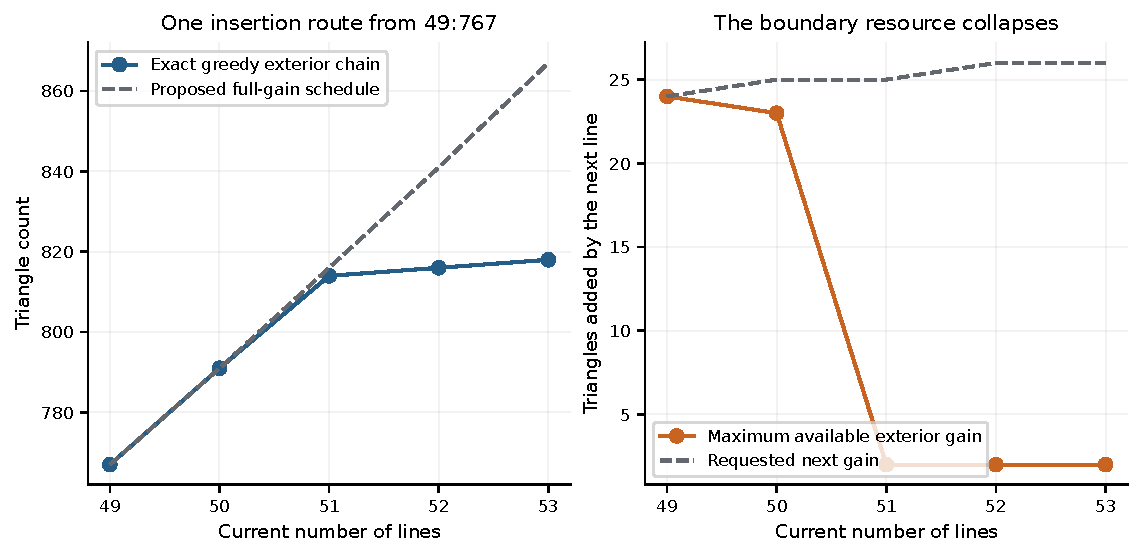
\includegraphics[width=0.88\linewidth]{figures/successor-49-resource.pdf}
\caption{The boundary resource in the particular exact 49-line chain.
The sharp drop in available wedges explains why its first full-gain
extension cannot be repeated with the requested next gain.  The plotted
capacities concern this chain only.}
\label{fig:successor}
\end{figure}

\subsection{A conditional recurrence and an unconditional numerical bound}

For any integer-valued function $F$, assume
\begin{equation}
 F(n+1)\geq F(n)+\lfloor n/2\rfloor\qquad(n\geq s).
 \label{ext:full-step}
\end{equation}
Summation, including both parity cases, gives the fully checked arithmetic
implication
\begin{equation}
 F(n)\geq F(s)+
 \left\lfloor\frac{(n-1)^2}{4}\right\rfloor-
 \left\lfloor\frac{(s-1)^2}{4}\right\rfloor
 \qquad(n\geq s).
 \label{ext:conditional-closed}
\end{equation}
The hypothesis \eqref{ext:full-step} remains explicit in the formal
theorem.  Substituting $s=49$ and $F(49)=767$ yields the numerical target
\begin{equation}
 Q_{49}(n)=\left\lfloor\frac{(n-1)^2}{4}\right\rfloor+191.
 \label{ext:49-target}
\end{equation}

There is now a separate unconditional Lean theorem
\begin{equation}
 \K(n)\geq Q_{49}(n)\qquad(n\geq49),
 \label{ext:49-unconditional}
\end{equation}
proved using the saved witnesses at 49 and 50 and the classical all-order
baseline thereafter.  Indeed, for $n\geq51$,
\[
 \frac{n(n-3)}3-\frac{(n-1)^2}4-191
 =\frac{n^2-6n-2295}{12}\geq0,
\]
with equality at $n=51$ and an increasing numerator beyond it.  Rounding
gives $\B(n)\geq Q_{49}(n)$.  This proves the desired numerical formula
without constructing a nested full-gain chain.  The stronger all-order
bound $\G$ and the finite envelope elsewhere in this paper also dominate
it.

For comparison, direct iteration of the defect rule
$T_{n+1}=T_n+g(n,T_n)$ from $49:767$ guarantees
$50:791$, $51:803$, $52:805$, and $60:821$.
The stronger target \eqref{ext:49-target} gives $51:816$, $52:841$, and
$60:1061$.  These are different constructions and different assertions.
The completed numerical theorem does not retrospectively prove the
March extension claim, and the failure of its proposed exterior
iteration does not invalidate the completed numerical theorem.

\section{Compatible seeds, geometric doubling, and sparse families}
\label{fam:section}

The second extension mechanism inserts a whole collection of lines near
a distinguished support.  It belongs to Bartholdi, Blanc, and Loisel
(BBL)~\cite{bbl2008}; it is fundamentally different from the one-line
exterior operation of Section~\ref{ext:section}.  The present work supplies
explicit compatible seeds, a recursively closed geometric Lean proof, and
finite certificates at considerably larger orders. The October release
completes both the odd iteration and the stronger adjacent-even family.
The numerical doubling gain retains its published attribution.

\subsection{The exact one-step theorem}

Let $q=4r$ with $r\geq5$, put $\alpha=\pi/q$, and take
\begin{equation}
  0<\varepsilon<\tan(\alpha/2).
  \label{fam:epsilon}
\end{equation}
Define $q$ ordered intercepts, indexed from zero, by
\begin{equation}
 a_j=
 \begin{cases}
 \tan((j-q/2+1)\alpha),&0\leq j<q/2-1,\\
 -\varepsilon,&j=q/2-1,\\
 \varepsilon,&j=q/2,\\
 \tan((j-q/2)\alpha),&q/2<j<q.
 \end{cases}
 \label{fam:old-grid}
\end{equation}
In particular, the extreme intercepts are $-\cot\alpha$ and
$\cot\alpha$.  The two central intercepts replace the repeated zero that
would otherwise occur in this grid.

\begin{definition}[Compatible tangent-grid seed]
\label{fam:compatible}
A seed at $(q,\varepsilon)$ consists of $Y_0:y=0$ and the $q$ lines
$L_j:y=m_j(x-a_j)$, with the following properties: the arrangement is
simple; every interval $[a_j,a_{j+1}]$ on $Y_0$ supports the triangular
cell with supports $Y_0,L_j,L_{j+1}$; and the central apex
$L_{q/2-1}\cap L_{q/2}$ lies above $Y_0$.  A counted seed additionally
carries a list of distinct actual triangular cells whose length is at
least $T$.
\end{definition}

Simplicity already requires all $m_j$ to be nonzero and pairwise distinct.
The distinguished-line condition is a substantial geometric restriction,
not a consequence of having a large total count.  It is precisely why
an arbitrary optimal arrangement cannot simply be used as a repeatable
BBL seed.

\begin{theorem}[Fully verified geometric doubling]
\label{fam:doubling}
Suppose $q=4r\geq20$ and \eqref{fam:epsilon} holds.  A compatible
tangent-grid seed with at least $T$ certified triangles gives a simple
real straight-line arrangement of $2q+1$ lines with at least
\begin{equation}
  T+q^2
  \label{fam:gain}
\end{equation}
triangles.
\end{theorem}

The precise formal theorem is \texttt{BBLDoubling.doubling}.  It assumes
the actual old line equations, simplicity, each distinguished triangle,
the positive central height, and a duplicate-free triangle list.  It
does not assume a future crossing order, a list of future empty
triangles, or a triangle-count recurrence.  Its conclusion is an actual
\texttt{SimpleLowerBound}; the generic proof uses only the standard Lean
logical axioms.  The numerical doubling principle is BBL's.  The
contribution here is its completed geometric proof for these explicit
hypotheses, using the following two-parameter realization.

\begin{proof}[Geometric proof and its formal decomposition]
For $0\leq i<q$ set
\[
 \beta_i=-\frac\pi2+(i+\tfrac12)\alpha,
 \qquad b_i=\tan\beta_i.
\]
Adjoin the lines
\begin{equation}
 M_i:\quad y=\kappa g_i(\delta)(x-b_i),\qquad
 g_i(\delta)=\frac{2b_i}{1+b_i^2}+\frac\delta{b_i}
            =\sin(2\beta_i)+\delta\cot\beta_i.
 \label{fam:pencil}
\end{equation}
Choose $\delta>0$ sufficiently small and then $\kappa>0$ sufficiently
small relative to the fixed $\delta$ and the seed.  This order of choices
is part of the proof.  BBL's published construction uses explicit scales;
the qualitative two-scale statement here is established independently
by the formal crossing analysis, rather than inferred from those fixed
scales.

For two new lines put $t=b_i$ and $u=b_k$.  Their intersection has
$x$-coordinate independent of $\kappa$:
\begin{equation}
 X_{ik}(\delta)=
 \frac{2tu(t+u)}{2tu(1-tu)-\delta(1+t^2)(1+u^2)}.
 \label{fam:crossing}
\end{equation}
When $tu\ne1$, its limit is the reduced tangent
$(t+u)/(1-tu)=\tan(\beta_i+\beta_k)$, and the exact displacement is
\begin{equation}
 X_{ik}(\delta)-\frac{t+u}{1-tu}
 =\frac{\delta(t+u)(1+t^2)(1+u^2)}
 {[2tu(1-tu)-\delta(1+t^2)(1+u^2)](1-tu)}.
 \label{fam:displacement}
\end{equation}
For sufficiently small positive $\delta$ its nonzero sign is that of
$(t+u)tu$.  If $tu=1$, the crossing diverges along the specified exterior
ray as $\delta\downarrow0$; if $t+u=0$, its coordinate is exactly zero.
Thus neither exceptional case is hidden inside a continuity argument
with a vanishing denominator.

The reduced tangents, the old intercepts, the new half-grid intercepts,
and $-\varepsilon,0,\varepsilon$ determine a strictly ordered finite
system of cuts.  Equations~\eqref{fam:crossing}--\eqref{fam:displacement}
place every new--new crossing in its prescribed cut interval.  Taking
$\delta$ in the intersection of the finitely many resulting positive
neighborhoods also makes the new slope factors nonzero and distinct.
For fixed such $\delta$, each old--new intersection tends to the
corresponding old intercept as $\kappa\to0$.  Finite continuity then
realizes all the prescribed strict crossing comparisons simultaneously.
Small $\kappa$ separates old and new slopes.  Injectivity along each new
crossing row excludes new triple intersections; old simplicity excludes
the remaining ones.  This proves actual simplicity and crossing order.

The count can now be separated from trigonometry.  Treat the $q$ new lines
and $Y_0$ as $q+1$ auxiliary supports.  The integer row model places old
support $j$ at key $4j+2$.  A pair of auxiliary supports with crossing key
$z$ yields a mixed triangle with old support $j$ when
\begin{equation}
  |z-(4j+2)|<4.
  \label{fam:neighbors}
\end{equation}
Every auxiliary pair has two such old neighbors, except for at most $q$
exterior pairs, each of which has one.  Hence the number is at least
\begin{equation}
 2\binom{q+1}{2}-q=q^2.
 \label{fam:mixed-count}
\end{equation}
The row inequalities make two sides consecutive on their supports.
The two-side emptiness lemma proves that the corresponding triangle is
an actual empty cell.  The supporting triples are distinct.  Thus
\eqref{fam:mixed-count} counts genuine triangles, not merely local
crossing patterns.

It remains to preserve the seed's contribution.  An old triangle not
using $Y_0$ has a strict half-plane sign against $Y_0$; all new lines
converge to $Y_0$, so its three vertex signs persist for sufficiently
small $\kappa$.  The old triangles with a side on $Y_0$ require a different
argument.  Saturation forces consecutive old apices to have opposite
heights.  The positive central apex fixes the alternating parity.
The crossing order identifies a new cap support for each noncentral
distinguished triangle.  On both cap endpoints, every new line has the
parity-correct weak sign; strict signs against other old supports
persist by continuity.  This replaces each such old triangle by one
empty triangle with the same two old supports.  The central triangle
itself is retained.  The finite cap and noncap requirements can again
be satisfied by one common positive $\kappa$.

Finally, these $T$ retained or replaced triangles have at least two old
nonhorizontal supports, while the $q^2$ mixed triangles have two
auxiliary supports.  The supporting triples cannot coincide.  Their
union is a duplicate-free witness of length at least $T+q^2$.
\end{proof}

The recurrence preserves the certified segment deficit:
\begin{equation}
 \Delta(q,T)=q^2-1-3T,\qquad
 \Delta(2q,T+q^2)=\Delta(q,T).
 \label{fam:deficit-preserved}
\end{equation}
Here the equality concerns the transported lower count; if the output
has additional uncounted triangles, its actual defect can be smaller.
Thus doubling amplifies a compatible seed to larger orders while
preserving its certified constant deficit.  A smaller-defect seed or a
new source of additional triangles is needed to improve that deficit.

\subsection{The compatible eleven-line realization}

The useful eleven-line count is $32$, an existing result; the search
started from the Honma-based construction displayed by
Savchuk~\cite{savchuk2025}.  The additional work here is an explicit
realization compatible with the BBL grid for arbitrarily small positive
central separation.  Take $Y_0:y=0$ and
\begin{equation}
 x-v_jy=a_j,\qquad
 (v_0,\ldots,v_9)=\tfrac1{10}(15,-2,14,1,4,-4,5,-3,12,-5),
 \label{fam:seed11-slopes}
\end{equation}
where
\begin{equation}
 (a_0,\ldots,a_9)=
 (-\tan\tfrac{4\pi}{10},-\tan\tfrac{3\pi}{10},
 -\tan\tfrac{2\pi}{10},-\tan\tfrac{\pi}{10},
 -\varepsilon,\varepsilon,
 \tan\tfrac{\pi}{10},\tan\tfrac{2\pi}{10},
 \tan\tfrac{3\pi}{10},\tan\tfrac{4\pi}{10}).
 \label{fam:seed11-grid}
\end{equation}
For every $0<\varepsilon\leq10^{-5}$ the seed is simple, has at least
32 certified triangles, and has all nine distinguished triangles.
Its central slopes are $5/2$ and $-5/2$ and its central height is
$5\varepsilon/2>0$.

The stability check is finite but uniform in $\varepsilon$.  The
determinant for a triple of nonhorizontal lines is affine in the
intercepts and therefore affine in $\varepsilon$:
\[
 D_{ijk}=(a_j-a_k)v_i+(a_k-a_i)v_j+(a_i-a_j)v_k.
\]
Exact rational enclosures for the four tangent values and endpoint
sign checks certify the whole interval.  The first certificate used
outward rational interval arithmetic; the subsequent Lean theorem uses
proved trigonometric enclosures and the parametric certificate soundness
theorem.  The limit $\varepsilon=0$ is used only to bound expressions;
it is not presented as a simple arrangement.  Five visible pairs for
$w=(10,-13)$ are also proved uniformly, giving the actual exterior bound
$12:37$ by Theorem~\ref{ext:realization}.

\begin{figure}[tb]
\centering
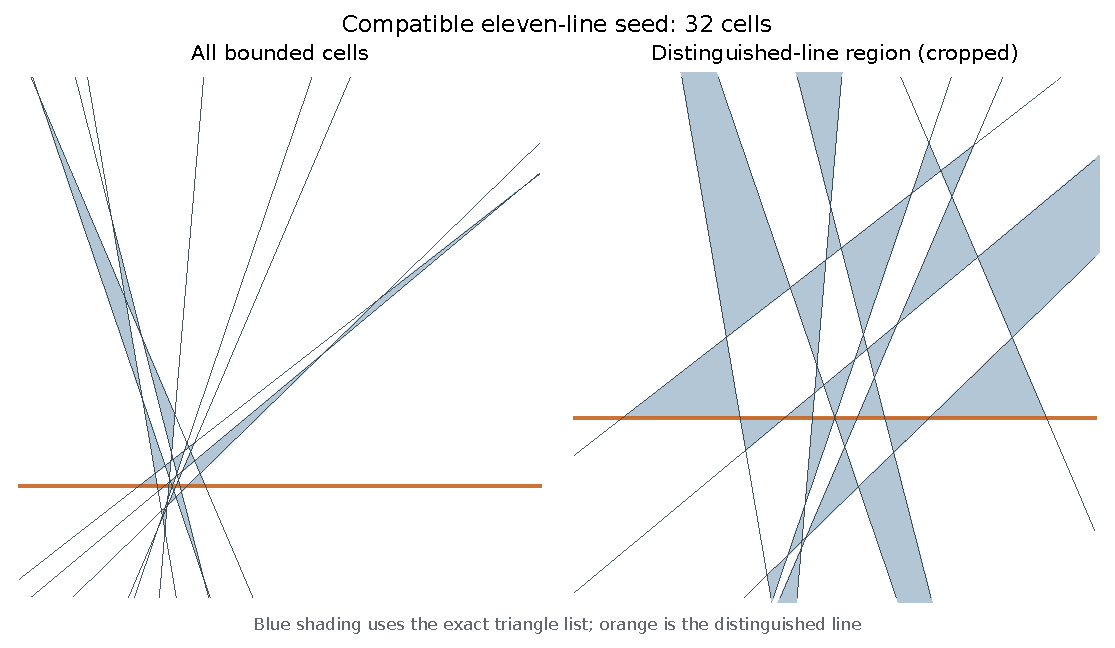
\includegraphics[width=0.88\linewidth]{figures/seed-11.pdf}
\caption{A finite rational realization of the compatible eleven-line
seed, with global and distinguished-line views.  The figure illustrates
the arrangement; the all-small-parameter
claim is certified by exact determinant and half-plane inequalities,
not by the rendering.  The count $32$ is inherited from earlier work;
the compatible realization and parameter certificate are the contribution
recorded here.}
\label{fig:seed11}
\end{figure}

\subsection{Closing the geometric invariant}

A numerical inequality after one step is insufficient for induction. The
output must again satisfy every geometric hypothesis in
Definition~\ref{fam:compatible}. The October construction returns precisely
that information. The \proofref{Kobon/BBLRecursiveSeed.lean}{11}{seed record}
contains actual slopes, a duplicate-free valid triangle list, simplicity,
every consecutive distinguished triangle, and the positive central apex.
The line labels are normalized by explicit inverse permutations; the
transport theorem preserves actual support triples and their triangle
predicates, rather than merely transporting a count.

\begin{theorem}[Closed geometric iteration]\label{fam:closed-iteration}
Fix $r\ge5$ and a counted seed size $T$. Suppose that for every sufficiently
small positive $\varepsilon$ a compatible tangent-grid seed with $4r+1$
lines and at least $T$ triangles exists. Then for every integer $t\ge0$
there is a simple arrangement of $4r\,2^t+1$ lines with at least $T_t$
triangles, where
\begin{equation}
 T_0=T,\qquad T_{t+1}=T_t+(4r\,2^t)^2,
 \qquad 3T_t+(4r)^2=3T+(4r\,2^t)^2.
 \label{fam:closed-count}
\end{equation}
At every finite depth the full seed invariant is available on some
nonempty positive parameter interval.
\end{theorem}

\begin{proof}
The geometric construction in Theorem~\ref{fam:doubling} is performed
while retaining the next distinguished triangles and the positive central
triangle. Its output intercepts, after the proved reindexing, are exactly
the tangent grid for $2r$. Simplicity and the counted list are carried in
the same witness. This is
\proofref{Kobon/BBLRecursiveSeed.lean}{61}{\lean{seed_step}}; its
coefficient identities are proved in \lean{BBLRecursiveGrid} and its
unreindexed geometric witness in \lean{BBLRecursiveWitness}.

More explicitly, let $\eta>0$ be a valid input threshold. The next seed
exists for every
\[
 0<\varepsilon<\min\{\eta,\tan(\pi/(8r))\}.
\]
The minimum is positive. For each such $\varepsilon$, the small pencil
parameters are chosen as in the one-step proof. No uniform lower bound
on these auxiliary parameters is needed. Thus the whole seed property,
including its nonempty interval, is preserved by $r\mapsto2r$.
Induction proves the first assertion and the recurrence. Multiplying
the recurrence by three and using $(2q)^2=q^2+3q^2$ proves the displayed
identity by induction. The formal results are
\proofref{Kobon/BBLInfinite.lean}{32}{\lean{uniform_iterate}},
\proofref{Kobon/BBLInfinite.lean}{46}{\lean{infinite_family}}, and
\proofref{Kobon/BBLInfinite.lean}{52}{\lean{triangleCount_identity}}.
\end{proof}

The quantifier is $\forall t\,\exists\eta_t>0\,\forall\varepsilon
\in(0,\eta_t)$, with a seed witness for each such parameter. It is not
$\exists\varepsilon>0\,\forall t$. In particular, the theorem does not
claim that a fixed drawn arrangement can be iterated with one fixed
positive gap forever. This distinction closes the earlier proof gap
without inserting an unproved compactness assertion.

The normalized 21-line seed supplies $r=5$, $T=132$ throughout
$0<\varepsilon\le10^{-5}$. Its nineteen distinguished triangles, actual
coefficient identity, and central height $5\varepsilon/2$ are proved in
\lean{BBLSeed21Normalized}. The generic theorem starts at $r\ge5$;
the separately verified eleven-line seed supplies the initial term in
the following family.

\begin{theorem}[Verified odd family]\label{fam:odd-verified}
For every integer $t\ge0$, set $q_t=10\cdot2^t$. Then
\begin{equation}
 \Ks(q_t+1)\ge T_t=\frac{100\cdot4^t-4}{3}
                    =\frac{q_t^2-4}{3}.
 \label{fam:eleven-family}
\end{equation}
\end{theorem}
\begin{proof}
For $t=0$ use the eleven-line certificate. For $t\ge1$ apply
Theorem~\ref{fam:closed-iteration} to the normalized 21-line seed at depth
$t-1$. Equation~\eqref{fam:closed-count} gives $3T_t+4=q_t^2$.
The exact formal declaration is
\proofref{Kobon/BBLVerifiedFamilies.lean}{24}{\lean{eleven_odd_family}}.
\end{proof}

The generic iteration uses only standard logical axioms. The concrete
family additionally inherits four existing native certificate checks
from its 21-line base. This is an unconditional geometric existence
theorem with an explicitly reported computation trust boundary, not a
conditional recurrence on unknown arrangements.

\subsection{Even companions and the retained boundary invariant}

The defect argument of Theorem~\ref{ext:defect-theorem} gives the weaker
ordinary mathematical consequence
\begin{equation}
 \Ks(q+2)\ge\frac{q^2-4}{3}+\frac q2-1,
 \qquad q=10\cdot2^t.
 \label{fam:even-defect}
\end{equation}
Indeed its gain is
$\lceil q(q-2)/(2(q+1))\rceil=q/2-1$. The October proof establishes the
additional visible pair at every depth, rather than extrapolating from
finite checkpoints.

A visible seed extends the preceding seed record by an admissible normal
$w=(w_x,w_y)$, a duplicate-free list of at least $V$ visible pairs, and a
rightmost old line $R$ satisfying
\[
 m_R>0,\qquad w_x+w_y m_R>0,
 \qquad x(R\cap L_i)\le a_R \quad(L_i\ne R).
\]
These are concrete line-intersection conditions. The record is
\proofref{Kobon/BBLVisibleSeed.lean}{7}{\lean{VisibleSeed}}. The generic
iteration additionally assumes $w_x>0$.

\begin{theorem}[Closed visible-boundary iteration]\label{fam:visible-iteration}
Under these uniform visible-seed hypotheses with $r\ge5$, doubling
preserves the normal and the whole visible-seed record, with
\begin{equation}
 (r,T,V)\longmapsto(2r,T+(4r)^2,V+2r).
 \label{fam:visible-step}
\end{equation}
Consequently, at depth $t$ the visible count satisfies
$V_t+2r=V+2r\,2^t$. If $V=2r$, the exterior extension yields at least
$T_t+2r\,2^t$ triangles at order $4r\,2^t+2$.
\end{theorem}

\begin{proof}
Old visible pairs avoiding $Y_0$ persist under a sufficiently small
pencil; at most one visible old pair uses $Y_0$. The new construction
supplies $r$ negative complementary pairs, $r-1$ positive
almost-complementary pairs, the pair of $Y_0$ and the rightmost new
support, and the pair of $R$ with the support at
$\beta_* =\pi/4-\alpha/2$. This supplies $2r+1$ pairs, compensating for
the possible old loss and leaving a gain of $2r$. Pair supports and
new/old tags prove that the retained list has no duplicates.

The last pair is controlled by
\[
 \cot\alpha\sin(2\beta)+\cos(2\beta)-1
   =\frac{\sin(2\beta+\alpha)}{\sin\alpha}-1.
\]
On the half-grid its unique maximum occurs at $\beta_*$, with a gap
at least $2\sin\alpha$. First shrink $\delta$ to preserve this strict
maximum, then shrink $\kappa$ to compare the actual new crossing with
all old vertices on $R$. The positivity of projected graph directions
transfers horizontal crossing order to $w$-order. The corresponding
rightmost clean ray is then established on the next grid. The finite
requirements are intersected with the eventual one-step witness, so the
same output has the old seed invariant and the new boundary invariant.

This is the geometric content of
\proofref{Kobon/BBLEvenStep.lean}{34}{\lean{canonical_visible_step}}
and \lean{BBLEvenRecursive.visible_seed_step};
\lean{BBLProjection}, \lean{BBLRightmost} and
\lean{BBLNextBoundary} supply the actual order and intersection lemmas.
Reindexing transports visibility and admissibility. The positive
parameter-interval induction is the same as for odd seeds. Summing
$V_{t+1}-V_t=2r\,2^t$ gives $V_t=V+2r(2^t-1)$. Finally apply the
proved exterior theorem to this actual visible-pair list.
\end{proof}

\begin{theorem}[Verified full-gain even family]
\label{fam:even-conditional}
For every integer $t\ge0$ and $q=10\cdot2^t$,
\begin{equation}
 \Ks(q+2)\ge\frac{q^2-4}{3}+\frac q2.
 \label{fam:even-strong}
\end{equation}
\end{theorem}
\begin{proof}
The normalized 21-line visible seed has $r=5$, $T=132$, $V=10$ and
$w=(10,-13)$. Its full rightmost-boundary and visibility hypotheses
hold uniformly for $0<\varepsilon\le10^{-5}$. Apply
Theorem~\ref{fam:visible-iteration}; the independently verified
$12:37$ witness supplies $t=0$. The unconditional declaration is
\proofref{Kobon/BBLVerifiedFamilies.lean}{51}{\lean{eleven_even_family}}.
Its dependencies include the four odd-seed native checks and two further
finite admissibility/visibility checks. No unresolved visibility
hypothesis remains in this concrete theorem.
\end{proof}

\begin{table}[tb]
\centering\small
\begin{tabular}{rrrrrl}
\toprule
$q$ & Odd order & Odd count & Even order & Even count & Family proof\\
\midrule
10&11&32&12&37&Lean existence\\
20&21&132&22&142&Lean existence\\
40&41&532&42&552&Lean existence\\
80&81&2132&82&2172&Lean existence\\
160&161&8532&162&8612&Lean existence\\
320&321&34132&322&34292&Lean existence\\
640&641&136532&642&136852&Lean existence\\
\bottomrule
\end{tabular}
\caption{The completed odd and even family. Every displayed existential
bound now follows from one general Lean theorem. This does not change
the separate verification status of previously exported coordinate files,
nor assert that these numbers exceed all literature constructions.}
\label{fam:finite-table}
\end{table}

\begin{figure}[tb]
\centering
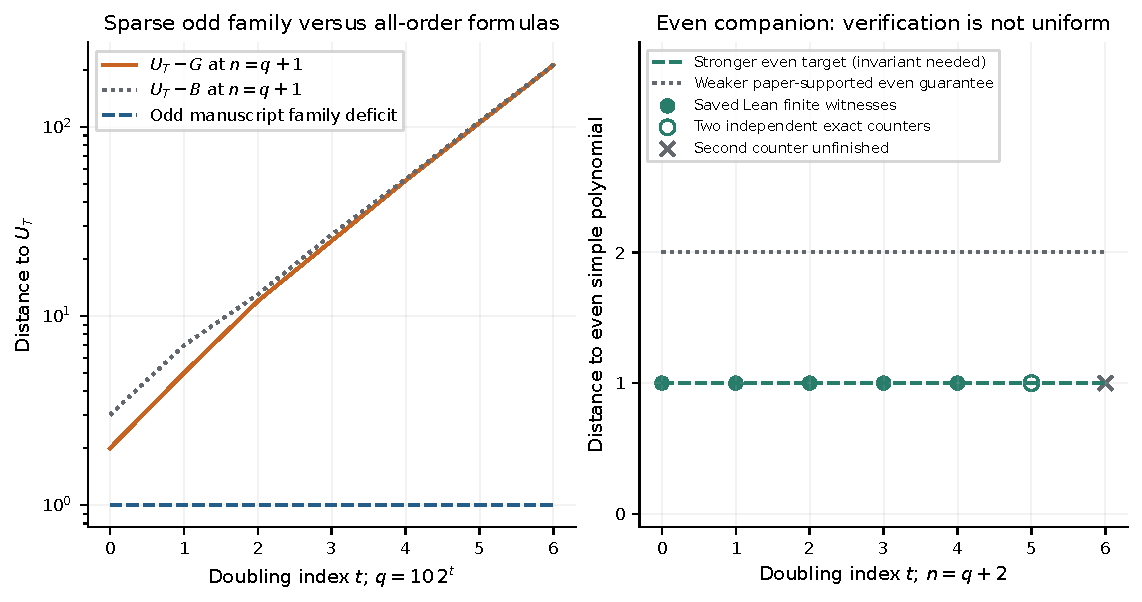
\includegraphics[width=0.88\linewidth]{figures/family-deficits.pdf}
\caption{The original sparse-family deficit plot, retained as a historical
numerical figure. Its arithmetic is unchanged. The family formulas now
have completed Lean existence proofs; any finite-check status encoded
in the original plot describes the September coordinate artifacts. The
new figure below compares the completed envelope.}
\label{fig:family-deficits}
\end{figure}

The independent adjacency and half-plane counters agree on the archived
321-, 322- and 641-line coordinate files, with $34132$, $34292$ and
$136532$ triangles. Their largest rational components have 916, 985 and
1103 decimal digits. The 642-line file passed adjacency and simplicity
checks but its separate direct recount was interrupted. That coordinate
artifact still has partial computational status. In contrast, existence
of some 642-line simple arrangement with at least $136852$ triangles is
now proved by Theorem~\ref{fam:even-conditional}. An existential proof
does not retrospectively certify the exact bytes of a saved coordinate
file.

\subsection{An improved verified bound at every natural order}

Recall the previous retained bound $\Lbound(n)=\max\{G(n),C(n)\}$ in
\eqref{eq:envelope}. Define the sparse family contribution
\begin{equation}
 R(n)=\begin{cases}
 (q_t^2-4)/3,& n=q_t+1,\\
 (q_t^2-4)/3+q_t/2,& n=q_t+2,\\
 0,&\text{otherwise},
 \end{cases}
 \qquad q_t=10\cdot2^t,
 \label{fam:sparse-bound}
\end{equation}
and put
\begin{equation}
 H(n)=\max\{\Lbound(n),R(n)\}.
 \label{fam:new-envelope}
\end{equation}
The two cases have different parity and each determines $t$ uniquely.
The executable Lean definition uses the maximum of the candidates for
$0\le t\le n$, rather than an infinite search.

\begin{theorem}[Total retained and recursive envelope]\label{fam:all-n-envelope}
For every $n\in\N$, $\K(n)\ge H(n)\ge\Lbound(n)$. For every $t\ge5$,
\begin{align}
 H(q_t+1)-\Lbound(q_t+1)&=\floor{q_t/3}-2,\\
 H(q_t+2)-\Lbound(q_t+2)&=q_t/2-\floor{q_t/3}-2,
 \label{fam:exact-gains}
\end{align}
and both differences are positive.
\end{theorem}
\begin{proof}
Each nonzero candidate in \eqref{fam:sparse-bound} has a simple witness
by the preceding two theorems, hence an unrestricted witness. The
finite maximum chooses one such witness or a retained finite/baseline
witness; it is not an addition of incompatible triangle counts. If a
candidate occurs at order $n$, then $t<2^t\le n$, so the executable
finite maximum includes it. This is
\proofref{Kobon/RecursiveEnvelope.lean}{51}{\lean{all_n}}.

Since $q_t^2\equiv1\pmod3$ and $q_t$ is even, substitution in $G$ gives
\[
 T_t-G(q_t+1)=\floor{q_t/3}-2,\qquad
 T_t+q_t/2-G(q_t+2)=q_t/2-\floor{q_t/3}-2.
\]
All saved finite enhancements end at order 195. Thus
$\Lbound(n)=G(n)$ for $n>195$, as proved by
\lean{BBLFamilyBenchmarks.previous_envelope}. For $t\ge5$,
$q_t\ge320$ and both differences are positive. The formal strict-tail
statement is \lean{RecursiveEnvelope.strict_previous_tail}; uniqueness
of the sparse candidate identifies $H$ with that candidate here.
\end{proof}

At 321 and 322 lines the gains over the old verified envelope are
respectively 104 and 52; at 641 and 642 they are 211 and 105. The first
members do not displace stronger retained certificates: $21:133$,
$22:143$, $41:533$ and $42:553$ remain in $H$. All 138 coordinate
identities and their published attribution are retained. This theorem
improves the previous verified repository envelope at infinitely many
orders. It does not prove a numerical record against all published
families, and its off-family values retain the preceding all-order
linear deficit.

\begin{figure}[tb]
\centering
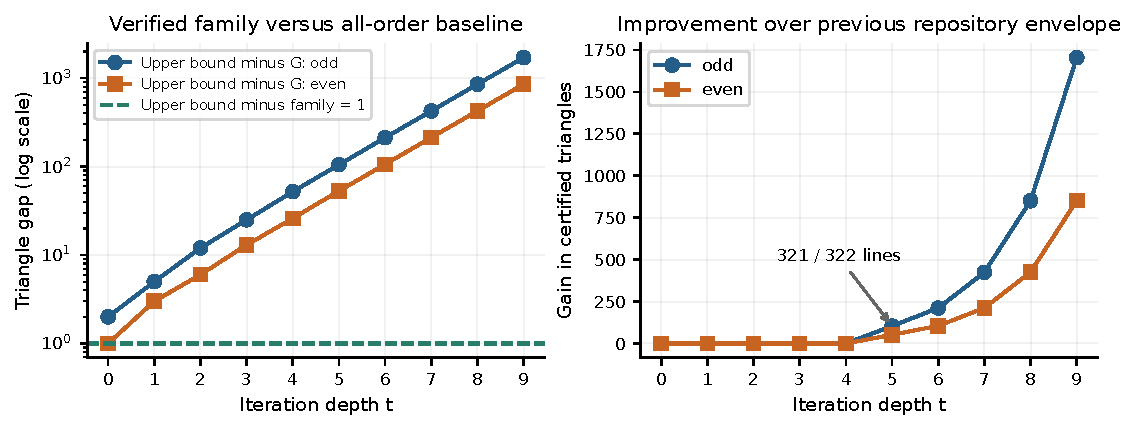
\includegraphics[width=0.95\linewidth]{figures/recursive-envelope.pdf}
\caption{The completed recursive family and the retained all-order bound.
The improvement is over the previous repository envelope; it is not a
numerical-priority comparison against all published constructions. The
upper comparisons refer to simple arrangements. Formula values are
proved in Lean; the plot is newly generated from those formulas.}
\label{fig:recursive-envelope}
\end{figure}

\subsection{Actual one-triangle optimality windows}

The October release also closes the geometric upper-bound bridge for
simple arrangements, as proved in Section~\ref{upper:simple-actual}.
This upgrades a comparison with a polynomial to a statement about the
actual extremal quantity.

\begin{corollary}[Simple optimality windows]\label{fam:optimality-windows}
For $q=10\cdot2^t$ and $t\ge0$, write $A=(q^2-4)/3$. Then
\begin{equation}
 A\le\Ks(q+1)\le A+1,\qquad
 A+q/2\le\Ks(q+2)\le A+q/2+1.
 \label{fam:windows}
\end{equation}
\end{corollary}
\begin{proof}
The lower halves are the constructed witnesses. For every simple
arrangement, the geometric upper results give
$3T\le n(n-2)$ and, for even $n\ge4$, $6T\le n(2n-5)$.
Substitution gives respectively
\[
 \floor{(q+1)(q-1)/3}=A+1,
 \qquad \floor{(q+2)(2q-1)/6}=A+q/2+1.
\]
The exact combined declarations are
\proofref{Kobon/BBLFamilyOptimality.lean}{29}{\lean{odd_window}} and
\proofref{Kobon/BBLFamilyOptimality.lean}{35}{\lean{even_window}}.
\end{proof}

The upper halves use standard logical axioms only; the lower halves
retain their seed's native dependencies. This one-triangle interval
need not be sharp at the smaller orders: the literature settles some
of them more precisely. In particular it is not an upper theorem for
arrangements with multiple concurrence, and it does not close the
unrestricted Kobon problem.

\subsection{Known optimal families and independent reproduction}

The classical dyadic five-line family must be kept separate from the
new compatible eleven-line realization.  A convenient normalized seed
uses intercepts $(-1,-\varepsilon,\varepsilon,1)$ and
\[
 x-v_jy=a_j,\qquad (v_0,v_1,v_2,v_3)=(-15,10,-10,30),
\]
together with $Y_0$.  The complete interval
$0<\varepsilon\leq10^{-5}$ has five certified triangles, all three
distinguished triangles, and two visible pairs.  Its central slopes
are $1/10$ and $-1/10$; the rightmost slope is $1/30$.
The normalization is deliberate: an earlier affine-equivalent numerical
realization had both central slopes negative, which was inadequate as
an unchecked premise for the sign convention in the published iterative
proof.  The corrected whole-parameter seed is verified in
\texttt{TamuraSeed5}.

The known optimal odd family and its simple even companions have
\begin{equation}
 q=4\cdot2^t,\qquad
 \Ks(q+1)\geq\frac{q^2-1}{3},\qquad
 \Ks(q+2)\geq\frac{q^2-1}{3}+\frac q2.
 \label{fam:tamura}
\end{equation}
The current finite certificates include
$5:5$, $6:7$, $9:21$, $10:25$, $17:85$, $18:93$, $33:341$,
$34:357$, $65:1365$, $66:1397$, $129:5461$, and $130:5525$.
These reproduce known numerical consequences of the affine family of
Forge and Ram\'irez Alfons\'in and BBL's odd-to-even discussion
\cite{forge1998,bbl2008}; they are not claimed as newly discovered
bounds.  Theorem~\ref{fam:doubling} as currently formalized does not
cover the small bases $q=4,8,16$, and the unfinished large parametric
33-line draft is not counted as a completed theorem.

Parpalak and Utkin supply a different straight-line family at
$q=18\cdot2^t$~\cite{parpalakutkin2026}.  Its odd count is
\begin{equation}
 \Ks(q+1)\geq\frac{q^2}{3}-1,
 \label{fam:pu}
\end{equation}
including $19:107$ and $37:431$.  The present work independently checked
their compatible 19-line seed on $0<\varepsilon\leq10^{-3}$ with 1632
exact endpoint determinant checks, a rational 107-triangle witness,
and all 17 distinguished triangles.  The interval reproduction is
separate from an end-to-end Lean proof of their infinite construction.
Both the seed and the family retain Parpalak--Utkin attribution.
The earlier BBL statement at $18\cdot2^t+1$ concerned pseudolines;
it cannot be used as a straight-line result without a realization
argument.  Applying Corollary~\ref{ext:odd-full} to the published
straight-line family gives the attributed simple even corollary
\[
 \Ks(q+2)\geq\frac{q^2}{3}+\frac q2-1,
\]
with $20:116$, $38:449$, $74:1763$, and $146:6983$.  Stronger nonsimple
published values at some of these orders concern $\K$, and do not
invalidate this simple-arrangement distinction.

\subsection{The former integration gap and the remaining seed branches}

The verified 21-line base has the true tangent intercepts
\eqref{fam:old-grid} with $q=20$, fixed rational slopes, 132 triangles,
19 distinguished triangles, ten visible pairs, and the required
rightmost-line property for every $0<\varepsilon\le10^{-5}$.
Its finite interval checks use native evaluation; their analytic and
geometric soundness proofs are proved separately.

\begin{figure}[tb]
\centering
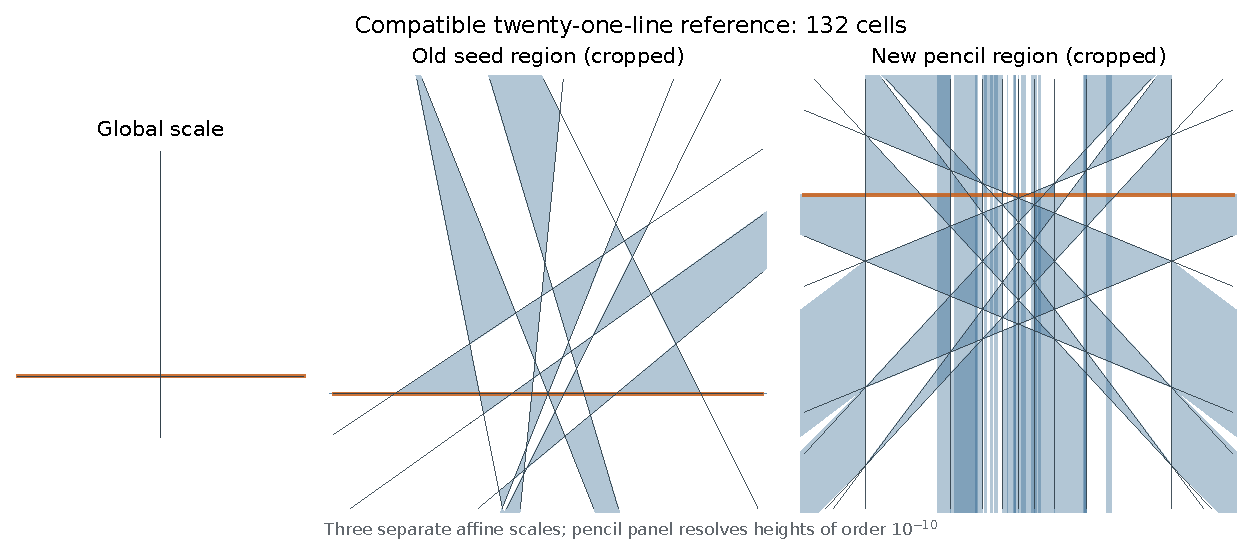
\includegraphics[width=0.88\linewidth]{figures/seed-21.pdf}
\caption{A 21-line hybrid checkpoint with 132 triangles. The global,
core and thin-pencil views illustrate scale separation. The finite
rendering is distinct from the true-tangent-grid parametric theorem in
\lean{BBLSeed21}. The normalized seed now starts the fully verified
recursion; the picture is not used as its proof.}
\label{fig:seed21}
\end{figure}

The September manuscript correctly identified four missing interfaces:
retained geometric data, whole-list transport under the next-grid
permutation, normalization of the 21-line grouped labels, and induction
on a positive parameter interval. All four are now complete. The
central source labels 5 and 6 have apex height $5\varepsilon/2$;
normalization preserves that actual point. The next central triangle
is retained independently of whether it appears in the counted list.
The invariant used in the successful induction is
\begin{equation}
 \exists\eta>0\quad\forall\varepsilon\in(0,\eta)\quad
 \exists\text{ a compatible counted seed at }(q,\varepsilon).
 \label{fam:recursive-quantifier}
\end{equation}
The former target
\begin{equation}
 q_t=20\cdot2^t,\qquad
 \Ks(q_t+1)\ge\frac{q_t^2-4}{3}
 \label{fam:21-target}
\end{equation}
is therefore a theorem, the tail of \eqref{fam:eleven-family}. The
visible-boundary interfaces are also closed by the same release.

This completion does not discharge every possible concrete seed.
For the Forge--Ram\'irez Alfons\'in branch, the active
\lean{BBLForgeConditional} proves the generic formulas
\[
 \Ks(32\cdot2^t+1)\ge\frac{1024\cdot4^t-1}{3},\qquad
 \Ks(32\cdot2^t+2)\ge\frac{1024\cdot4^t-1}{3}+16\cdot2^t
\]
under the explicit premises \texttt{UniformSeed 8 341} and its visible
analogue. The large concrete 33-line uniform base and its dependent
sources remain excluded drafts: the full native check did not finish.
Finite certificates at 33, 34, 65, 66, 129 and 130 remain valid. A
finite base at one parameter is not the uniform base premise above.

\subsection{A uniform 49-line compatibility certificate}
\label{fam:seed49}

The October search found a stronger compatible seed at order 49 using
fixed rational reciprocal slopes of denominator $10^{10}$. Its 48
intercepts are
\[
 -\tan\frac{23\pi}{48},\ldots,-\tan\frac\pi{48},
 -\varepsilon,\varepsilon,
 \tan\frac\pi{48},\ldots,\tan\frac{23\pi}{48}.
\]
Exact rational interval arithmetic verifies, throughout
$0<\varepsilon\le1/100$, a simple arrangement with 767 certified
triangles, all 47 distinguished-line caps and a positive central apex.
The fixed normal $(1,-2)$ has 24 visible pairs, including rightmost
pair $(0,48,49)$; the last slope is $1/3$ and the required boundary
inequalities hold uniformly. These are exact external certificate
claims, not completed finite Lean base theorems.

The analytic part is now inside Lean:
\sourcefile{Kobon/BBLTangent48Bounds.lean}{\lean{BBLTangent48Bounds}}
proves rational enclosures for each of the 23 positive tangent values,
using half-angle and reciprocal identities beginning with
$\tan(\pi/3)=\sqrt3$. The endpoint widths are at most
$5\cdot10^{-36}$. The exported finite predicates were independently
replayed: 1,176 direction checks, 18,424 simplicity checks, 37,583
triangle/support checks and 1,176 visibility/support checks passed.
Two independent exact cell counters also find 767 triangles at the
rational midpoint witness. None of these facts is a substitute for the
unfinished Lean evaluation of the full parametric base.

\begin{figure}[tb]
\centering
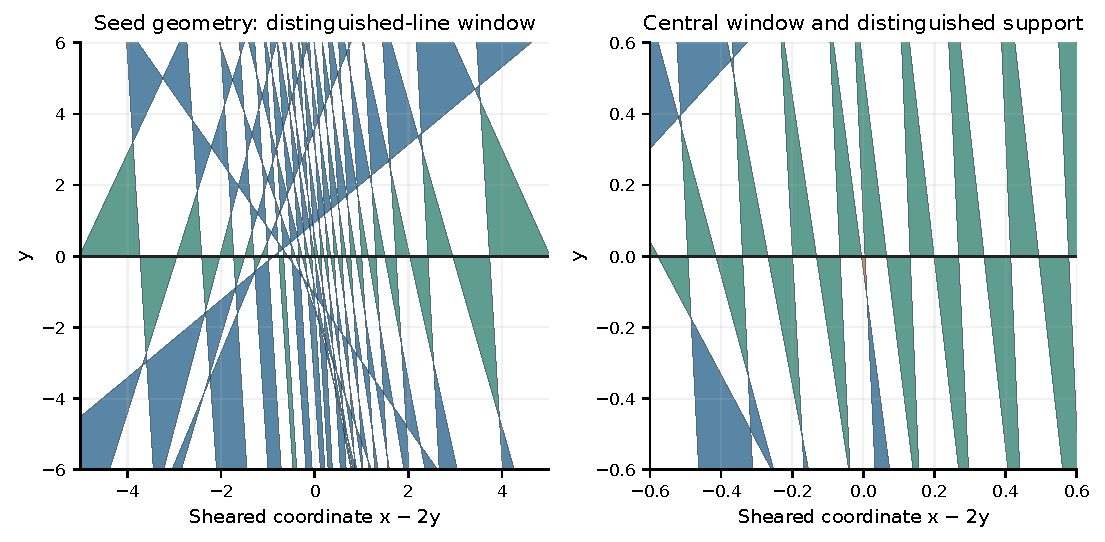
\includegraphics[width=0.98\linewidth]{figures/uniform49.pdf}
\caption{Two clipped windows of the rational midpoint witness for the
uniform 49-line seed, with $\varepsilon=1/200$. The invertible shear
$x'=x-2y$ makes the distinguished structure easier to see. The left
window has $x'\in[-5,5]$, $y\in[-6,6]$; the right has both coordinates
in $[-0.6,0.6]$. Ordinary certified cells are blue, distinguished caps
teal and the central cell orange. Distant cells lie outside these
windows: the panels do not display all 767 triangles. The uniform
certificate is exact external evidence; full Lean seed integration
remains incomplete.}
\label{fig:uniform49}
\end{figure}

If this uniform seed is promoted into the proved recursive interface,
its counts will be
\begin{equation}
 q=48\cdot2^t,\qquad T_{\rm odd}=768\cdot4^t-1,
 \qquad T_{\rm even}=768\cdot4^t+24\cdot2^t-1
 \label{fam:49-conditional}
\end{equation}
at orders $q+1$ and $q+2$. The odd formula is exactly the tail $s=t+3$
of BBL's Theorem~1.3 for $n=6\cdot2^s+1$~\cite{bbl2008}; these are
not new numerical records. The contribution of this branch is an
explicit, well-conditioned uniform compatibility certificate and a
partially completed formal linkage. Five dependent seed/family files
are visibly excluded as unverified drafts. Isolated tangent, graph and
arithmetic proofs do not make the full base proof complete.

Earlier positive-margin fits had moved triangles across infinity.
The successful fit additionally preserves the original affine sign
system. This illustrates why incidence or a projective order type alone
cannot certify the desired affine cell count.

A preceding search for a perfect compatible 21-line seed tested
11,547,910 floating proposals and 3,234 linear-feasibility programs
without improving 132. Those bounded failures were not impossibility
proofs. The exact obstruction in Section~\ref{exp:grid-obstruction}
now proves a much more precise limitation for a prescribed grid and
supplied classification; it still does not exclude other compatible
families or a different geometric construction.

\section{Multiplicity-sensitive upper-bound arguments}
\label{upper:scope}

This section develops upper estimates by separating the ordinary part of an arrangement from its finite multiple points. The October release completes extraction of actual elementary segments, their incidence identity and clean-line charging for pairwise nonparallel arrangements. It also proves the classical simple upper bounds from actual witnesses. The remaining global cyclic-fan extraction is stated explicitly: conditional core-budget arithmetic is not an unrestricted Lean upper theorem. None of the restricted estimates below is claimed as a new numerical upper bound for the full function $\K$.

The distinction is necessary because the even-order estimates of Bartholdi--Blanc--Loisel and Blanc require simplicity~\citep{bbl2008,blanc2011}. The classical Cl\'ement--Bader envelope is treated as a reported external theorem~\citep{clementbader2007}; the local example in Section~\ref{upper:shared-fan} explains why we do not silently replace its proof by a bound on all shared edges incident to a multiple point.

\subsection{An exact elementary-segment identity}

\begin{definition}
For an arrangement of $n$ distinct affine lines, let $t_r$ be the number of finite intersection points incident to exactly $r$ lines, and let $P$ be the number of unordered parallel pairs. A bounded \emph{elementary segment} is the portion of an arrangement line between two consecutive finite intersection points. Let $E$ count these segments, $U$ count those incident to no triangular cell, and $D$ count those incident to two triangular cells. Let $a$ be the number of lines containing at least one finite intersection point, and put
\[
 S=\sum_{r\ge3}r(r-2)t_r,\qquad
 \delta=n(n-2)-3T,
\]
where $T$ is the number of bounded triangular cells.
\end{definition}

\begin{proposition}[Segment and defect identities]
\label{upper:identity}
For every such arrangement,
\begin{align}
 E&=n(n-1)-2P-S-a,\\
 3T&=E-U+D,\\
 \delta&=2P+S+a-n+U-D.
 \label{upper:defect-general}
\end{align}
If every line meets another line, then $a=n$ and $\delta=2P+S+U-D$.
\end{proposition}

\begin{proof}
Each nonparallel unordered pair contributes to exactly one finite point, so
\[
 n(n-1)-2P=\sum_{r\ge2}r(r-1)t_r.
\]
If a line has $s>0$ distinct finite intersection points, it contributes $s-1$ bounded elementary segments; an isolated line contributes none. Summing point-line incidences gives
\[
 E=\sum_{r\ge2}r t_r-a.
\]
Subtracting these expressions yields the first identity. Each triangular cell uses three elementary segments. A segment is incident to zero, one, or two such cells, so the total number of triangle-side incidences is $E-U+D$. Substitution into the definition of $\delta$ gives the last identity.
\end{proof}

The term $D$ cannot be dropped in a nonsimple arrangement. Multiple points reduce the available segment count by $S$, but sharing can compensate for some of that loss. This is precisely the interaction that a classical upper proof must control.

\begin{lemma}[A shared side has a multiple endpoint]
\label{upper:shared-endpoint}
An elementary segment incident to two bounded triangular cells cannot have both endpoints ordinary, where an ordinary point is incident to exactly two arrangement lines.
\end{lemma}

\begin{proof}
At each ordinary endpoint there is a unique supporting line other than the line containing the segment. Both adjacent triangles would therefore have the same three supporting lines. Three distinct lines have at most one bounded triangular region, whereas the two incident cells lie on opposite sides of the shared segment. This is impossible.
\end{proof}

For the remainder of the section assume that $n\ge4$ is even and that all pairs of lines are nonparallel. Let the \emph{core} consist of the finite points of multiplicity at least three. Write
\[
 q=\sum_{r\ge3}t_r,\qquad I=\sum_{r\ge3}r t_r,
\]
and let $h$ count the lines meeting the core. Let $D_1$ count shared elementary segments with exactly one core endpoint and $D_2$ those with two core endpoints. By Lemma~\ref{upper:shared-endpoint}, $D=D_1+D_2$, and hence
\begin{equation}
 \delta=S+U-D_1-D_2.
 \label{upper:core-identity}
\end{equation}

\subsection{Parity on a line outside the core}

A line is \emph{clean} if it contains no core point. The following argument adapts the local parity method in Blanc's Section~2~\citep{blanc2011}. Its proof is included because the transverse lines may have multiple intersections away from the clean line.

\begin{lemma}[Clean-line charging]
\label{upper:clean-charge}
For even $n\ge4$ and pairwise nonparallel lines,
\begin{equation}
 n-h\le2U+D_1.
 \label{upper:charging}
\end{equation}
\end{lemma}

\begin{proof}
First fix a clean line $L$, place it horizontally, and number its $n-1$ crossings from left to right. Let $R_i$ be the transverse line at crossing $i$. Denote the bounded segment of $L$ between crossings $i$ and $i+1$ by $\ell_i$, and its two exterior rays by $\ell_0$ and $\ell_{n-1}$. Write $p_i^+$ and $p_i^-$ for the faces above and below $\ell_i$, and $r_i^+,r_i^-$ for the elementary transverse pieces of $R_i$ immediately above and below $L$. A transverse piece may be a bounded segment or an unbounded ray.

We show that some bounded $r_i^{\pm}$ is unused or shared. Suppose otherwise: every bounded transverse piece is incident to exactly one triangle. Each bounded $\ell_i$ is unshared by Lemma~\ref{upper:shared-endpoint}.

If both $p_1^+$ and $p_1^-$ are nontriangular, then $r_1^+$ and $r_1^-$ are unused: their other adjacent faces meet the exterior ray $\ell_0$. At least one of these transverse pieces is bounded, because $R_1$ meets another transverse line. This contradicts the supposition. Reflecting across $L$ if necessary, assume $p_1^+$ is triangular; $p_1^-$ is then not.

For $1\le i\le n-2$, prove the following assertions together:
\begin{enumerate}[label=(\roman*)]
\item if $i$ is even, $p_i^+$ is nontriangular; if $i$ is odd, $p_i^-$ is nontriangular;
\item if both faces at $\ell_{i-1}$ are nontriangular, then $p_i^-$ is triangular for even $i$, and $p_i^+$ is triangular for odd $i$.
\end{enumerate}
The base case follows from the choice of $p_1^+$ and the unbounded faces at $\ell_0$. Consider an even step; the odd step exchanges signs. If $p_{i-1}^+$ is triangular, then $p_i^+$ cannot be triangular, since otherwise the two triangles share the bounded piece $r_i^+$, contrary to the supposition. Assertion (ii) has a false antecedent in this case.

Otherwise both $p_{i-1}^+$ and $p_{i-1}^-$ are nontriangular by the preceding odd step. This cannot happen for $i=2$, so $i\ge4$. The earlier even step makes $p_{i-2}^+$ nontriangular. Hence $r_{i-1}^+$ is unused, and must be unbounded. The intersection of $R_{i-1}$ and $R_i$ must consequently lie below $L$. It follows that $r_i^-$ is bounded. Its left adjacent face is nontriangular, so its right adjacent face $p_i^-$ must be triangular. Since $\ell_i$ is unshared, $p_i^+$ is nontriangular. This proves both assertions.

Now $n-2$ is even, so $p_{n-2}^+$ is nontriangular. If $p_{n-2}^-$ is also nontriangular, both pieces at the last crossing are unused and at least one is bounded, again a contradiction. Otherwise $p_1^+$ and $p_{n-2}^-$ are triangular, while $r_1^-$ and $r_{n-1}^+$ are unused. The lines $R_1$ and $R_{n-1}$ intersect. If their intersection is below $L$, then $r_1^-$ is bounded; if above, then $r_{n-1}^+$ is bounded. This is the final contradiction.

Charge each clean line to one bounded unused or shared transverse segment supplied by this argument. An unused segment can receive at most two charges, one at each ordinary endpoint. A shared segment must have a multiple endpoint, so it can receive at most one charge if counted by $D_1$, and none if counted by $D_2$. There are $n-h$ clean lines, giving~\eqref{upper:charging}.
\end{proof}

\begin{remark}[Why parallel pairs have been excluded]
Three parallel vertical lines and one horizontal line give a clean horizontal line whose transverse pieces are all unbounded. Thus simply removing parallel-participating lines from the set to be charged does not prove the lemma. The identities of Proposition~\ref{upper:identity} allow parallels, but the charging argument above does not. Every subsequent upper estimate in this section retains the pairwise nonparallel hypothesis.
\end{remark}

Combining~\eqref{upper:core-identity} and~\eqref{upper:charging} gives the basic budget
\begin{equation}
 2\delta\ge n+2S-h-3D_1-2D_2.
 \label{upper:basic-budget}
\end{equation}
The remaining problem is to bound the shared-side contribution at the core.

\subsection{The geometric obstruction in a cyclic fan}

At an $r$-fold point $v$, the incident lines determine $2r$ rays in cyclic order, with opposite rays separated by $r$ positions. Let $d_1(v)$ count shared elementary segments starting at $v$ and ending at an ordinary point, and let $d_2(v)$ count those ending at another core point. A ray supports at most one such incident elementary segment.

\begin{lemma}[No long run of ordinary-ended shared rays]
\label{upper:no-long-run}
For $r\ge3$, no $r-1$ consecutive rays at an $r$-fold point can all support segments counted by $d_1(v)$.
\end{lemma}

\begin{proof}
Such a run would border $r$ consecutive triangular sectors. At the ordinary endpoint of each selected shared segment, the opposite supporting lines of the two neighboring triangles must coincide: besides the radial line through $v$, only one arrangement line passes through that endpoint. Propagating this equality makes the opposite sides of all $r$ triangles lie on one line $M$.

The line $M$ would meet $r+1$ consecutive rays from $v$, which include an opposite pair. A line meeting both open opposite rays must contain their connecting segment and hence $v$. But the opposite side of a nondegenerate triangle with vertex $v$ cannot lie on a line through $v$. This contradiction proves the lemma.
\end{proof}

This is an actual geometric statement, not an assumed combinatorial prohibition. The Lean module \texttt{FanGeometry} proves uniqueness and propagation of opposite supports for real lines and points. The module \texttt{CyclicFan} supplies the cyclic-to-geometric bridge from triangular sectors, antipodal rays and ordinary selected endpoints.

\begin{proposition}[Local fan budget]
\label{upper:fan-budget}
At every finite point of multiplicity $r\ge3$,
\begin{equation}
 d_1(v)\le2r-3,\qquad 3d_1(v)+d_2(v)\le6r-6.
 \label{upper:local-fan-budget}
\end{equation}
\end{proposition}

\begin{proof}
Count selected rays in all $2r$ cyclic windows of length $r-1$. Each window contains at most $r-2$ selected rays by Lemma~\ref{upper:no-long-run}, and each selected ray belongs to exactly $r-1$ windows. Therefore
\[
 (r-1)d_1(v)\le2r(r-2).
\]
If $d_1(v)\ge2r-2$, the left side is at least $2(r-1)^2=2r(r-2)+2$, a contradiction. Finally $d_1(v)+d_2(v)\le2r$, so
\[
 3d_1(v)+d_2(v)=2d_1(v)+(d_1(v)+d_2(v))\le6r-6.
\]
\end{proof}

The cyclic double count is proved in \texttt{FanCount}. The theorem \lean{CyclicFan.selected_card_le} combines it with the real geometric obstruction, without assuming the no-long-run conclusion as an unexplained premise.

\subsection{A weighted bound for an arbitrary finite core}

\begin{proposition}[Multiplicity-weighted defect estimate; manuscript geometry]
\label{upper:weighted}
Let $n\ge4$ be even and let the arrangement be pairwise nonparallel. Then
\begin{equation}
 2\delta\ge n+\sum_{r\ge3}(2r^2-11r+6)t_r.
 \label{upper:weighted-defect}
\end{equation}
\end{proposition}

\begin{proof}
Each $D_1$ segment has exactly one core endpoint and each $D_2$ segment has two. Summing~\eqref{upper:local-fan-budget} gives
\[
 3D_1+2D_2\le6I-6q.
\]
Also $h\le I$, since every core line contributes at least one point-line incidence. Inserting both inequalities into~\eqref{upper:basic-budget} yields
\[
 2\delta\ge n+2S-7I+6q,
\]
which is~\eqref{upper:weighted-defect} after expanding $S,I,q$.
\end{proof}

The local weights are $-9,-6,1,12,27$ at multiplicities $3,4,5,6,7$, respectively. Consequently the obstruction to recovering a simple-style parity defect is concentrated at triple and quadruple points; higher multiplicity has a positive weight in this accounting.

\begin{corollary}[Nonnegative core weight; manuscript geometry]
\label{upper:high-multiplicity}
Under the hypotheses of Proposition~\ref{upper:weighted}, if
\[
 \sum_{r\ge3}(2r^2-11r+6)t_r\ge0,
\]
then
\[
 T\le\left\lfloor\frac{n(n-5/2)}3\right\rfloor.
\]
In particular, this holds if every finite multiple point has multiplicity at least five.
\end{corollary}

\begin{proof}
The weighted estimate implies $\delta\ge n/2$, giving the displayed upper bound by the definition of $\delta$. For $r\ge5$, the exact factorization
\[
 2r^2-11r+6=1+(r-5)(2r-1)\ge1
\]
proves the stated sufficient condition.
\end{proof}

This extends the same polynomial to a restricted nonsimple class. It says nothing comparable for a general core consisting of many triple points. Numerical first priority for this restricted consequence has not been established.

\subsection{A sharper estimate with at most two core points}

\begin{lemma}[A fan with at most one core-to-core ray]
\label{upper:one-core-ray}
If $d_2(v)\le1$ at a point of multiplicity $r\ge3$, then $d_1(v)\le2r-4$.
\end{lemma}

\begin{proof}
Mark which of the $2r$ sectors at $v$ are triangular. A ray supports a shared elementary segment exactly when both neighboring sectors are triangular. If every sector is triangular, every ray is shared; deleting at most one $d_2$ ray leaves a run of at least $2r-1$ selected rays, contradicting Lemma~\ref{upper:no-long-run}. Hence a nontriangular sector exists.

Suppose $d_1(v)\ge2r-3$. Two separated nontriangular sectors exclude at least four shared rays, as do three consecutive nontriangular sectors. Both situations are impossible. If exactly one sector is nontriangular, the shared rays form a path of length $2r-2$. Deleting at most one $d_2$ ray leaves at most two selected runs. Their total capacity is $2(r-2)$, less than the required $2r-3$. If exactly two adjacent sectors are nontriangular, at most $2r-3$ shared rays remain. All would have to be selected, forming a run of length $2r-3>r-2$. These cases exhaust the possibilities and prove the lemma.
\end{proof}

\begin{theorem}[At most two finite multiple points; manuscript geometry]
\label{upper:two-core}
An arrangement of an even number $n\ge4$ of pairwise nonparallel affine lines with at most two finite multiple points satisfies
\begin{equation}
 T\le\left\lfloor\frac{n(n-5/2)}3\right\rfloor+1.
 \label{upper:two-core-upper}
\end{equation}
More precisely, the defect bounds are $\delta\ge n/2$ if $q=0$, $\delta\ge n/2-1$ if $q=1$, and $\delta\ge n/2-3$ if $q\le2$.
\end{theorem}

\begin{proof}
With at most two core points, at most one ray at a core point can terminate at another core point. Lemma~\ref{upper:one-core-ray} gives $D_1\le2I-4q$. There is at most one core-to-core shared segment, so $D_2\le q(q-1)/2\le1$. Moreover,
\[
 h\le I-D_2,
\]
because any such segment lies on a line counted twice in the core-incidence total and once among the core lines. Substitution in~\eqref{upper:basic-budget} yields
\[
 2\delta\ge n+\sum_{r\ge3}(2r^2-11r+12)t_r-D_2.
\]
For $r\ge3$,
\[
 2r^2-11r+12=-3+(r-3)(2r-5)\ge-3.
\]
Thus $2\delta\ge n-3q-D_2\ge n-7$. Since $n$ and $2\delta$ are even, $2\delta\ge n-6$. Rearranging gives~\eqref{upper:two-core-upper}. If $q=1$, then $D_2=0$ and the inequality $2\delta\ge n-3$ rounds to $2\delta\ge n-2$; if $q=0$, it gives $2\delta\ge n$ directly.
\end{proof}

The hypotheses are attained by externally attributed exact constructions. Table~\ref{upper:restricted-attainment} records examples whose pairwise nonparallel status, triangle count, and two triple points were checked exactly. Their equality with~\eqref{upper:two-core-upper} proves sharpness within this restricted class, not optimality over all classical arrangements.

\begin{table}[htbp]
\centering\small
\begin{tabular}{@{}rrrl@{}}
\toprule
$n$ & $T$ & Restricted upper & Coordinate provenance\\
\midrule
8 & 15 & 15 & Earlier construction, retained in the current gallery\\
14 & 54 & 54 & Maiorana, two-triple-point witnesses\\
26 & 204 & 204 & Parpalak--Utkin gallery\\
50 & 792 & 792 & Parpalak--Utkin gallery\\
\bottomrule
\end{tabular}
\caption{Attainment in the class covered by Theorem~\ref{upper:two-core}. Sources: \citet{maiorana2026,parpalakutkinGallery2026}. These are not new numerical records claimed by this paper.}
\label{upper:restricted-attainment}
\end{table}

ProofAtlas reports a stronger restriction-specific result at $n=14$, covering up to four finite multiple points~\citep{proofatlas2026}. Its proof was not independently reproduced here. Our two-point estimate covers all even orders and arbitrary core multiplicities, but neither that fact nor the table establishes priority for the restricted theorem.

\subsection{A checked shared-fan example and the limits of smoothing}
\label{upper:shared-fan}

Consider the six lines
\begin{equation}
 x=0,\quad y=0,\quad x+y=3,\quad x-y=0,\quad
 2x+y=3,\quad x+2y=3.
 \label{upper:median-lines}
\end{equation}
They are the three sides of a triangle and its three medians. There are six bounded triangular cells and four triple points. At $v=(1,1)$, six distinct nonzero elementary radial segments are shared sides, each belonging to two of those cells. Three have ordinary other endpoints and three have multiple other endpoints, giving $d_1(v)=d_2(v)=3$; globally $D_1=D_2=3$.

\begin{figure}[htbp]
\centering
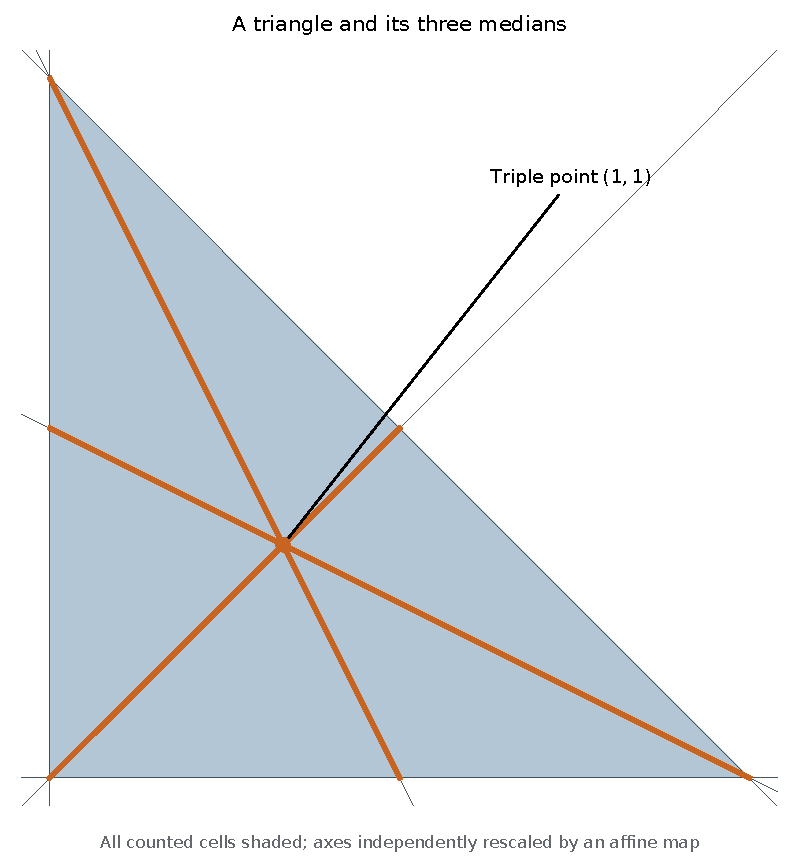
\includegraphics[width=0.75\textwidth]{figures/shared-fan.pdf}
\caption{The exact arrangement~\eqref{upper:median-lines}. Six triangular cells meet around the central triple point, and all six radial sides are shared. This refutes only a literal local incidence reading of the shared-pair statement in Cl\'ement--Bader's Lemma~1; it does not refute their final upper theorem. The figure is newly generated from the integer equations.}
\label{fig:shared-fan}
\end{figure}

The \texttt{SharedFan} module proves the real geometric facts: each designated triangle has nonempty uncut interior, the six interiors are pairwise disjoint, the radial segments are distinct and elementary, and each is a side of two distinct triangles. The proof uses ordinary kernel checking.

This matters when interpreting the Cl\'ement--Bader proof. Its local shared-pair sentence cannot literally bound all shared segments incident to a multiple point by two. An intended assignment of each shared side to one endpoint would be a different assertion requiring global justification. The example has only six triangles, below the reported seven-triangle upper bound at order six; it is therefore not a counterexample to that upper theorem. The present paper leaves that distinction explicit and uses the separate $D_1,D_2$ accounting instead.

Nor can one justify a simple upper bound merely by perturbing every multiple point. For a retained two-triple-point Maiorana $14{:}54$ witness, the four local generic resolution types have triangle counts $52,52,53,52$. These counts were checked with exact arithmetic; they are finite experimental evidence, not a new Lean theorem classifying all perturbations. They demonstrate why a universally nondecreasing smoothing argument needs more than the existence of a small generic perturbation. Our global upper argument never assumes such monotonicity.

\subsection{Actual arrangement extraction and simple upper theorems}
\label{upper:simple-actual}

The formal inventory is now built from an actual finite injective family
of certified triangles in $n\ge2$ pairwise nonparallel lines. It may
be a proper subset of all triangular cells. The quantities $U,D_1,D_2$
are defined relative to this selected family. The cell theorem proves
interior disjointness, and the side-emptiness theorem proves that each
side has consecutive endpoints on its supporting line.

An unordered endpoint pair represents one geometric side. At most two
pairwise interior-disjoint nondegenerate triangles can share that side:
three would put two on the same side of its support, forcing their
interiors to overlap near an interior base point. Counting triangle-side
incidences therefore gives $3T=E-U+D_1+D_2$. Pair counting proves
$\sum r(r-1)t_r=n(n-1)$ and the actual consecutive-edge inventory gives
$E=n(n-2)-S$. Thus
\begin{equation}
 \delta=S+U-D_1-D_2
 \label{upper:actual-identity}
\end{equation}
is proved from geometry by
\sourcefile{Kobon/UpperEdgeInventory.lean}{\lean{certificate_defect_identity}};
capacity, incidence and edge cardinality are conclusions of the proof,
not assumed numerical identities.

\begin{theorem}[Actual clean-line charging and simple bounds]
\label{upper:actual-simple}
Let $n\ge4$ be even. For any pairwise nonparallel real arrangement and
finite injective certified triangle family,
\begin{equation}
 n-h\le2U+D_1.
 \label{upper:actual-charging}
\end{equation}
For every simple arrangement with $T$ certified triangular cells,
\begin{equation}
 3T\le n(n-2)\quad(n\ge2),\qquad
 6T\le n(2n-5)\quad(n\ge4\text{ even}).
 \label{upper:actual-simple-bounds}
\end{equation}
\end{theorem}

\begin{proof}
The parity proof of Lemma~\ref{upper:clean-charge} can also be organized
as an odd-cardinality matching contradiction, which is the formal route.
A clean line has exactly $n-1$ distinct crossings. One common open
half-plane contains a further crossing on every transverse support.
Choose in that half-plane the consecutive bounded segment incident to
each clean-line crossing. Existence is obtained from the nearest actual
intersection, with the bounded-side and uniqueness lemmas handling
both signs.

If every chosen edge had degree one in the certified triangle family,
its unique triangle would have its base on the clean line: at an ordinary
crossing a triangle must use one of the two incident supports. Consecutive
edge uniqueness and interior disjointness then make these bases a
disjoint two-element cover of the clean-line crossings. Such a cover
has even cardinality, contradicting $n-1$ odd. Hence some incident
bounded edge has degree zero or two. A degree-two edge has a multiple
other endpoint by the shared-side lemma, so it is counted by $D_1$.

Choose one resulting charge for each clean line. A fixed ordinary
endpoint of an edge determines at most one clean transverse line.
An unused edge has at most two such endpoints and receives at most two
charges; a $D_1$ edge has exactly one ordinary endpoint and receives
at most one. This proves \eqref{upper:actual-charging}. The extraction,
choice and fiber bounds are all in
\proofref{Kobon/UpperCleanCharging.lean}{100}{\lean{certificate_clean_line_budget}},
using \lean{UpperCleanHalfplane}, \lean{UpperCleanEdges},
\lean{UpperCleanPairing} and \lean{UpperCleanCover}. No charge-existence
or pairing premise remains.

For a simple arrangement the core is empty, so $S=D_1=D_2=h=0$.
Equation~\eqref{upper:actual-identity} gives $3T=n(n-2)-U$, proving the
first bound. In the even case $n\le2U$, so
$6T=2n(n-2)-2U\le n(2n-5)$.
The \lean{SimpleLowerBound} versions extract the injective finite family
from its duplicate-free triangle list. These are
\sourcefile{Kobon/UpperSimpleOptimality.lean}{\lean{simple_lower_bound_upper}}
and
\sourcefile{Kobon/UpperEvenSimpleOptimality.lean}{\lean{simple_lower_bound_even_upper}}.
\end{proof}

The integer floor forms follow immediately. These classical inequalities
retain their earlier attribution, including Blanc's even parity bound.
Their contribution here is a complete real-geometric formalization with
standard logical axioms only. In particular, the retained simple
$44:608$ certificate attains $\lfloor44(88-5)/6\rfloor=608$; this
proves simple optimality at that order, not unrestricted optimality.
Theorem~\ref{upper:actual-simple} does not justify applying the even
polynomial to nonsimple witnesses such as $14:54$.

\subsection{Extremal fans and strengthened local restrictions}
\label{upper:extremal-fans}

\begin{theorem}[Equality structure of a supplied cyclic fan]
\label{upper:extremal-structure}
Consider actual local sector data at an $r$-fold point, $r\ge3$, satisfying
the cyclic order, antipodality, triangle and ordinary-endpoint conditions
of \lean{UpperFan.Sectors}. If $d_1=2r-3$, every sector is triangular
and $d_2=3$. Consequently,
\begin{equation}
 d_2\le2\Longrightarrow d_1\le2r-4,
 \qquad 3d_1+d_2\le6r-8+2e,
 \label{upper:extremal-weight}
\end{equation}
where $e=1$ when $d_1=2r-3$ and $e=0$ otherwise.
\end{theorem}

\begin{proof}
The no-long-run property from Lemma~\ref{upper:no-long-run} holds for
the selected ordinary-ended shared rays. If a sector were missing,
both bounding rays would be absent from that selected set. The cyclic
window count with these adjacent omissions strengthens its cardinality
bound to $2r-4$. Thus the extremal case has every sector present; all
$2r$ rays are then shared. Subtracting $d_1=2r-3$ gives $d_2=3$.
If $d_2\le2$, equality in the old bound is therefore impossible.
In the nonextremal case,
$3d_1+d_2=2d_1+(d_1+d_2)\le2(2r-4)+2r$; in the extremal case its
value is $6r-6$. These give \eqref{upper:extremal-weight}.
The exact proofs are
\proofref{Kobon/UpperFan.lean}{171}{\lean{all_sectors_of_extremal}},
\proofref{Kobon/UpperFan.lean}{187}{\lean{core_shared_card_eq_three_of_extremal}}
and \proofref{Kobon/UpperFan.lean}{227}{\lean{weighted_local_bound}}.
\end{proof}

This strengthens the previous manuscript's local hypothesis $d_2\le1$
to $d_2\le2$. The theorem's supplied local interface must still be
extracted from every core in a whole arrangement before summation.
Two further geometric restrictions are proved with their interfaces
explicit. A supported extreme core cannot carry the full extremal fan
when its core-ended rays are identified with points in the supporting
closed half-plane (\lean{UpperFanSupport} and
\lean{UpperCoreBoundary}). Also, two full extremal triple fans cannot
be adjacent across the same matched elementary side with its two
neighboring certified triangles (\lean{UpperTripleFan}). The latter
uses the actual coincident endpoints and opposing adjacent sectors;
an arbitrary pair of abstract fan records need not supply that matching.

\subsection{Core budgets: completed inputs and the precise conditional step}

Actual extraction now proves
\begin{equation}
 D_2+h\le I,\qquad D_2\le\binom q2,\qquad
 2S-7I+15q\ge0.
 \label{upper:core-inputs}
\end{equation}
The first inequality counts consecutive core vertices on each support;
the second maps a core-to-core elementary edge injectively to its two
endpoints; the last sums $2r(r-2)-7r+15=(r-3)(2r-5)\ge0$ over core
multiplicities $r\ge3$. They are proved in
\lean{UpperCoreLineIncidence} and \lean{UpperCoreCombinatorics}.

If a globally extracted family supplies the local bounds in
\eqref{upper:extremal-weight}, summation gives
$3D_1+2D_2\le6I-8q+2e$, where $e$ counts exceptional full fans.
Combining this with the actual defect and charging identities proves
\begin{equation}
 2\delta\ge n+2S-7I+8q-2e+D_2.
 \label{upper:refined-conditional}
\end{equation}
This is
\proofref{Kobon/UpperCoreBudget.lean}{47}{\lean{weighted_defect_with_core_edges}}.
The fan-summation premise is explicit; the equation is not yet a general
Lean theorem on every nonsimple arrangement.

For at most three core points each core has at most two possible core
neighbors. Once the missing ray/edge identification supplies
$D_1\le2I-4q$, the actual inputs above and $D_2\le3$ imply, at $n=2m$,
\begin{equation}
 \delta\ge m-6,\qquad
 T\le\floor{m(4m-5)/3}+2.
 \label{upper:three-core-conditional}
\end{equation}
For completeness, the algebra is short. Twice the defect and charging
give $2\delta\ge2m+2S-h-3D_1-2D_2$. Substitute
$h\le I-D_2$ and $D_1\le2I-4q$ to get
$2\delta\ge2m+2S-7I+12q-D_2\ge2m-3q-D_2\ge2m-12$.
Substitute $\delta=2m(2m-2)-3T$ and take the integer floor.
\proofref{Kobon/UpperCoreBudget.lean}{58}{\lean{at_most_three_multiple_points}}
checks these inequalities while retaining the needed fan premise.

\subsection{Formal status and the remaining global bridge}

\begin{longtable}{@{}P{0.32\linewidth}P{0.63\linewidth}@{}}
\caption{Current upper-proof boundary. All completed sources use standard
logical axioms; conditional implications retain the displayed premises.}
\label{upper:formal-status}\\
\toprule Component & Status in the October release\\\midrule\endfirsthead
\toprule Component & Status in the October release\\\midrule\endhead
\bottomrule\endfoot
Triangle-side geometry & Actual elementary sides, at-most-two capacity and
certified-cell disjointness completed.\\
Edge inventory and core & Actual multiplicity identity, consecutive-edge
cardinality, shared endpoint classification and defect identity completed.\\
Clean-line charging & Actual bounded charge existence, odd-crossing parity
contradiction, choice and finite charge fibers completed.\\
Simple upper bounds & Both classical polynomial inequalities and their floor
forms completed from actual simple witnesses.\\
Local fan structure & No long run, equality structure, supported-core and
matched triple-fan obstructions completed for explicit local interfaces.\\
Core incidence & Actual $D_2+h\le I$, $D_2\le\binom q2$ and nonnegative
multiplicity surplus completed.\\
Global fan extraction & Canonical cyclic ray order, actual multiplicity,
endpoint/edge correspondence, and shared-triangle matching remain open.\\
Restricted core upper formulas & Ordinary geometric arguments or conditional
Lean arithmetic; no unqualified whole-arrangement theorem is claimed.\\
Parallel classes & General elementary accounting is included on paper;
formal charging retains the nonparallel hypothesis.\\
\end{longtable}

The older \lean{CleanLineBudget} contains implications with symbolic
parallel-pair terms. These do not prove the missing parallel charging
lemma. Likewise, the exact checks on 597 test arrangements and the
imported gallery/ Maiorana witnesses support and debug the accounting,
but do not replace its geometric proofs. Completing global fan
extraction would certify the restricted conclusions with their intended
hypotheses. A new unrestricted numerical upper bound requires further
mathematical control of the entire low-multiplicity core.

\section{Exact certificates, external reproduction, and unsuccessful searches}
\label{exp:section}

The experimental program serves two purposes: producing concrete coordinate
witnesses for lower bounds, and identifying which proposed general arguments
survive exact checks. These purposes require different standards of evidence.
A successful coordinate witness proves an existential lower bound at its
specified order. A failed search ordinarily proves neither an upper bound nor
the nonexistence of a better construction. This section records both positive
and negative outcomes without merging their logical scopes.

\subsection{From a numerical proposal to an exact geometric witness}

The stored coordinates use the convention $a_ix+b_iy=c_i$, with rational or
integer coefficients. Each line is normalized to a primitive integer triple.
Pair intersections are computed as homogeneous integer triples, normalized
with a positive final coordinate. Consequently, collinearity, concurrence,
parallelism, and comparisons along a supporting line can all be tested without
floating-point tolerances.

Two independently implemented counters are used. The first sorts the distinct
intersection vertices on each line and constructs the graph of elementary
bounded segments; a three-cycle supported by three different lines is a
triangular cell. The second enumerates support triples and tests whether every
other line has a common weak sign at their three vertices. Nonzero area and
the distinction between open interiors and boundaries are checked explicitly.
Where a complete independent verification is reported, both counters agree on
the triangle set, not merely on a rounded area or a visual estimate. The Lean
geometric soundness theorem provides a third, logically separate link from
accepted coordinate predicates to real affine triangles.

Numerical optimization is used only to propose coordinates or rank candidate
chambers. A proposal is rationalized and recounted before promotion. In the
phase/chart experiments, progressively finer integer scales were accepted only
when the entire exact triangle set and simplicity were retained. Such a finite
acceptance does not prove that an arbitrary rounding of an irrational
construction is valid. The real all-order theorem for $\G$ has its own
determinant, trigonometric, and counting proof.

The released catalog contains 138 distinct promoted coordinate identities.
Several identities can occur at the same order and triangle count, and an
identity may have several repository source paths. Thus 138 is a catalog size,
not a count of new records or independent discoveries. The complete catalog
in Table~\ref{exp:catalog} includes simple versus nonsimple status, provenance
collections, and coordinate-hash prefixes; its machine-readable companion
records full hashes, source paths, and theorem modules. The finite Lean
certificates use native evaluation where indicated. This trust boundary is
broader than that of the universal construction, whose proof uses only Lean's
standard logical axioms.

\subsection{Finite improvements relative to the retained collection}

The phase and affine-chart work raised the preceding saved values at eleven
orders:
\[
\begin{array}{c|rrrrrrrrrrr}
n&39&47&48&51&53&54&55&59&60&99&195\\\hline
\text{previous}&469&690&720&817&884&918&954&1102&1140&3169&12481\\
\text{current}&470&691&721&818&885&919&955&1103&1141&3170&12482
\end{array}
\]
Each row is an improvement over the project's preceding retained coordinate
catalog. The underlying trigonometric family is due to
F\"uredi--Pal\'asti~\cite{furedipalasti1984}; these comparisons do not establish
numerical first priority. The general formula $\G$ now explains all eleven
displayed counts. The first projective search reached $47:691$ after 11,264
proposals; the subsequent exposed-cap description replaced that search by a
direct construction and an all-order proof.

The earlier OEIS-attributed values $28:238$, $30:275$, and $34:357$ remain
independently certified~\cite{oeisA006066,zarzuelo2026}. The drawings in this
paper render the currently retained exact witnesses, obtained by exterior
extension of retained odd-order inputs. They are not asserted to be literal
reproductions of the March diagrams. Likewise, the historical inventory in
Table~\ref{exp:historical} preserves earlier outputs without upgrading every
original derivation to a completed general theorem.

The current strongest saved simple and classical coordinate counts for every
$3\leq n\leq60$ appear in Table~\ref{exp:finite-table}. An absent entry in the
explicit OEIS table is recorded as a dash. Absence from that table is not
evidence that a value is absent from the literature; conversely, a coordinate
certificate does not establish optimality without an upper theorem covering
the same arrangement class.

\subsection{Independent reproduction of external constructions}

The current Parpalak--Utkin coordinate gallery~\cite{parpalakutkin2026} supplied
exact witnesses at
\[
\begin{gathered}
8:15,\quad14:54,\quad20:117,\quad26:204,\quad32:315,\\
36:402,\quad38:450,\quad42:553,\quad46:667,\quad50:792.
\end{gathered}
\]
Both independent counters reproduced their triangle sets. These witnesses
retain their source attribution; in particular, the eight-line numerical
value has older discovery priority than the coordinate gallery. Their addition
to this repository improves its verified coverage, not the discoverer's
claim to the numbers. The inspected gallery snapshot is commit
\texttt{feae4f5571a988a3ed45bd26a36259ebb7d7d3d2}.

All fifteen of Andrea Maiorana's published $14:54$ coordinate
configurations~\cite{maiorana2026} were also independently checked. Fourteen
have exactly two triple points, and one has four; none has a parallel pair.
The source snapshot is commit
\texttt{e47c7cfd9661e54d29befb83118bf83d5f804028}. Its CC BY 4.0 licence,
original coordinate files, and source attribution are retained. Added wrappers
record counts and verification metadata. This reproduction imports no claim
that a simple-arrangement upper theorem applies to these nonsimple witnesses.

These examples also expose a concrete limitation of smoothing. In Maiorana's
first example, the triple supports are $\{0,4,10\}$ and $\{0,11,12\}$.
Independently shifting the offsets of lines 4 and 11 by $\pm1/1000$ realizes all
four local resolution choices while preserving every originally nonzero
determinant sign. The resulting triangle counts are $52,52,53,52$, all below
54. Thus the proposed nondecreasing local smoothing strategy fails even when
the local sign choices are independently realizable by straight lines. The
argument identifying these sign choices with all sufficiently small local
resolutions is an ordinary finite sign-stability argument, not a completed
Lean theorem.

For the gallery's collinear-core examples at orders
$8,14,20,26,32,38,50$, all 132 recorded local resolutions were realized by
exact private-line offsets. Their respective best simple counts were
$14,51,114,203,313,448,791$. In particular, a universal claim that resolving
such a core loses at most one triangle is also false. Figure~\ref{fig:external-comparison}
separates these finite obstructions from any general upper-bound assertion.

\begin{figure}[tbp]
  \centering
  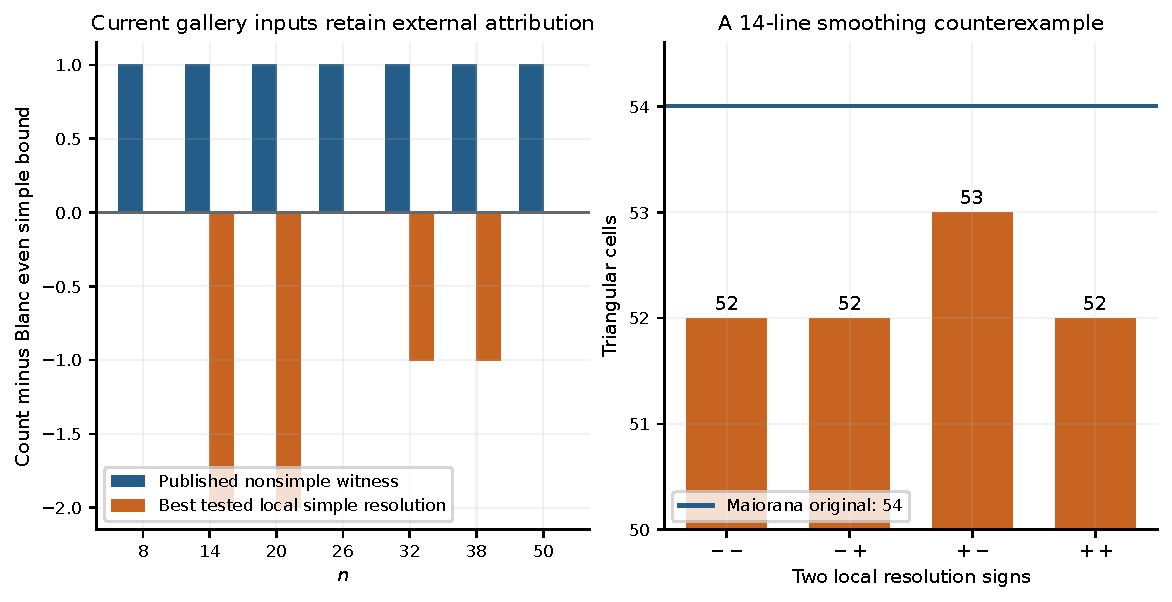
\includegraphics[width=\textwidth]{figures/external-comparison.pdf}
  \caption{Exact local-resolution tests on attributed external constructions.
  Left: Parpalak--Utkin gallery witnesses and their best tested simple local
  resolutions, measured relative to Blanc's even simple-arrangement polynomial;
  the eight-line value has older priority. Right: all four local resolutions of
  Maiorana's two-triple-point $14:54$ example. The original arrangements are
  nonsimple, so exceeding the simple polynomial is consistent. These are
  smoothing obstructions, not upper bounds for the classical problem.}
  \label{fig:external-comparison}
\end{figure}

\subsection{Projective charts, algebraic curves, and chamber searches}

Projective geometry provides a useful global neighborhood: changing the line
at infinity moves all lines together and may bound formerly unbounded
triangular faces. It can also lose bounded cells. For the exact saved
$81:2132$ and $161:8532$ hybrid arrangements, the projective triangular-face
census already equals their bounded-cell count; a chart change alone cannot
increase those particular counts.

Exact rational linear-arithmetic searches give sharper restrictions for some
fixed configurations. The nine-line half-phase rational arrangement has 21
projective triangular faces, but the recorded QF\_LRA solver result rules out a
chart retaining all 21. Similar fixed-seed tests find no gain for the tested
half-phase arrangements at $14,20,26,44$, and no chart retaining all 471
projective triangles of the saved $39:470$ witness. For a nonuniform cubic
48-line seed with 724 projective triangles, 2,903 exact linear-arithmetic checks
rule out 722 bounded triangles within the tested chart-retention formulation.
These are exact-solver results about specified rational seeds. Their UNSAT
certificates have not been independently checked in Lean, and they are not
global upper bounds at those orders.

The algebraic-curve direction tested both nodal-cubic angle perturbations and
torsion cosets on real elliptic curves. A larger projective face count did not
automatically produce a better affine construction. For the better two-real-
component elliptic examples, the projective, original affine, and best found
affine counts were respectively
\[
\begin{array}{c|rrrr}
n&42&48&54&60\\\hline
\text{projective}&550&724&922&1144\\
\text{original affine}&538&710&907&1127\\
\text{best found affine}&539&712&908&1129
\end{array}
\]
All fall below the corresponding retained affine bounds. The chart scans at
54 and 60 had 90-second limits. Numerical ranking and bounded running time
preclude a global nonexistence inference.

Oriented-matroid mutations and kinetic chamber sweeps addressed a different
limitation: moving inside a fixed projective type cannot create new
projective triangular faces. The mutation searches changed determinant signs,
using linear-programming realization where appropriate. Kinetic sweeps varied
many offsets, or both slopes and offsets, and visited concurrency events along
selected rays. Their event counts are not counts of all realizable order
types, and unsuccessful floating rays were discarded. Figure~\ref{fig:negative-searches}
records effort without treating heterogeneous search units as comparable
coverage measures.

\begin{figure}[tbp]
  \centering
  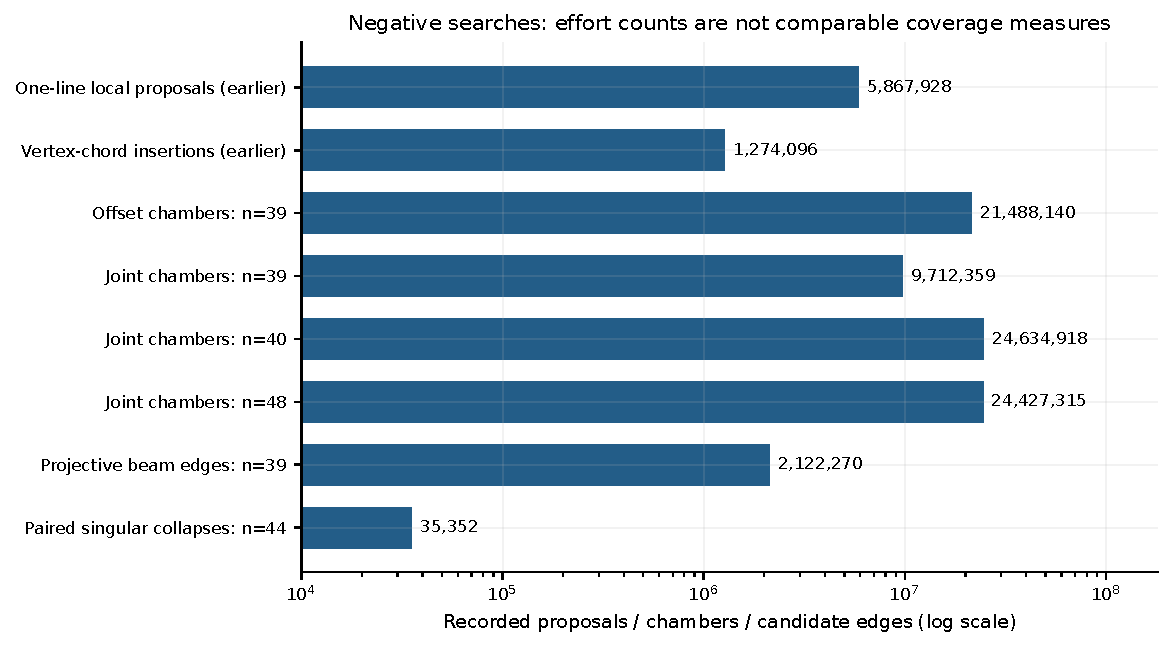
\includegraphics[width=\textwidth]{figures/negative-searches.pdf}
  \caption{Selected unsuccessful searches, with their recorded units.
  Proposal, chamber, and candidate-edge totals describe different search
  neighborhoods. They do not measure exhaustive coverage, justify an upper
  bound, or rank the mathematical promise of the methods. All proposed
  improvements would require subsequent exact geometric verification.}
  \label{fig:negative-searches}
\end{figure}

The final 39-line projective beam examined 2,122,270 candidate edges through
4,559 states without exceeding 470 affine or 471 projective triangles, even
at its combinatorial scoring stage. The 48-line LP walk accepted 471 mutations
out of 511 attempts and retained 721 affine and 724 projective triangles.
At 44 lines, singular-boundary searches included 35,352 paired collapses;
the retained beam checkpoint had 771 states and 446,422 candidate edges,
without exceeding 608. An unfinished round was discarded. These results
motivate a change of neighborhood or a structural argument rather than
repeating the same local searches.

Other bounded approaches included Fourier deformations (2,687,600 proposals
in one 39-line run), partial deletions from BBL constructions, and constrained
tangent-grid transfer by LP/MILP. The tested optimal 23-line chart transfers
did not admit a positive-margin realization on the desired grid; a constrained
near-optimal search gave 144 triangles, below a separately known compatible
145. None of these observations proves nonexistence of another compatible
seed or a different successful deletion pattern.

\subsection{A proved algebraic obstruction to tangent-grid transfer}
\label{exp:grid-obstruction}

The October search connects oriented-matroid sign constraints, linear
programming duality and exact algebraic number arithmetic. For the
reciprocal-coordinate lines $x-v_i y=a_i$, a prescribed determinant
sign becomes a strict linear inequality in the unknown reciprocal
slopes. Write
\begin{equation}
 D_{ijk}=(a_j-a_k)v_i+(a_k-a_i)v_j+(a_i-a_j)v_k.
 \label{exp:linear-determinant}
\end{equation}
Once the intercepts are fixed, feasibility is a linear sign problem,
even though the intercepts themselves are algebraic.

\begin{lemma}[Positive-dependence obstruction]\label{exp:farkas}
Let $A_i\in\R^d$ and let $\lambda_i\ge0$, with at least one
$\lambda_i>0$, satisfy $\sum_i\lambda_i A_i=0$. There is no $v\in\R^d$
with $A_i\mathbin{\cdot}v>0$ for every $i$.
\end{lemma}
\begin{proof}
Taking the scalar product with $v$ makes the left side a positive
weighted sum, but the assumed vector identity makes it zero. This
classical strict alternative is formalized by
\sourcefile{Kobon/StrictLinearCertificate.lean}{\lean{homogeneous_infeasible}}.
The formal theorem also provides an affine form for nonhomogeneous
strict systems.
\end{proof}

Set $t=\tan(\pi/20)$. Its exact algebraic specification is
\begin{equation}
 p(t)=t^4-4t^3-14t^2-4t+1=0,
 \qquad \frac3{20}<t<\frac{17}{100}.
 \label{exp:quartic}
\end{equation}
The quintuple-angle identity with $\tan(5\pi/20)=1$ gives
$(t-1)p(t)=0$; the interval excludes $t=1$. Monotonicity on the interval
identifies the intended root. \lean{BBLTangentAlgebra} proves the
quartic, root interval and uniqueness; \lean{BBLTangentValues} proves
that its explicit cubic power-basis expressions are the actual nine
values $\tan(k\pi/20)$ for $1\le k\le9$. Thus replacing trigonometric
numbers by algebraic expressions does not insert a numerical guess.

Use the actual 20-intercept grid
\[
 a_j=\begin{cases}
 -\tan((9-j)\pi/20),&0\le j<9,\\
 -\varepsilon,&j=9,\\
 \varepsilon,&j=10,\\
 \tan((j-10)\pi/20),&11\le j<20.
 \end{cases}
\]
The following ten prescribed signs are impossible.

\begin{theorem}[One exact tangent-grid obstruction]
\label{exp:actual-grid-obstruction}
For every real $\varepsilon$ and every real vector
$(v_0,\ldots,v_{19})$, at least one row of
Table~\ref{exp:ten-signs} fails the strict inequality
$s_iD_{j_i k_i\ell_i}>0$.
\end{theorem}

\begin{table}[tb]
\centering\small
\begin{tabular}{@{}cll@{}}
\toprule
Support triple & $s_i$ & Positive multiplier $\lambda_i(t)$\\
\midrule
$(0,6,15)$ & $-1$ & $-20t^3+120t^2+300t-40$\\
$(0,7,13)$ & $+1$ & $-8t^3+24t^2+96t+8$\\
$(0,8,14)$ & $-1$ & $-45t^3+205t^2+555t-35$\\
$(0,13,19)$ & $+1$ & $-16t^3-6t^2+40t+2$\\
$(3,6,8)$ & $+1$ & $20t^3-100t^2-220t+100$\\
$(3,11,15)$ & $-1$ & $20t^3-120t^2-220t+200$\\
$(3,13,17)$ & $+1$ & $20t^3-150t^2-300t+130$\\
$(7,11,13)$ & $+1$ & $-60t^3+240t^2+860t+320$\\
$(8,14,17)$ & $-1$ & $-105t^3+455t^2+1275t-45$\\
$(8,15,19)$ & $-1$ & $36t^3-188t^2-452t+124$\\
\bottomrule
\end{tabular}
\caption{An explicit positive linear-dependence certificate. Indices are
zero-based intercept indices. The rows use eleven distinct intercepts
and avoid the two exceptional central indices. Each column of the
weighted signed coefficient matrix vanishes modulo $p(t)$.}
\label{exp:ten-signs}
\end{table}

\begin{proof}
For each row define $A_i$ to be the coefficient vector of $s_iD$ in
\eqref{exp:linear-determinant}. All ten displayed multipliers are
positive throughout $3/20<t<17/100$, by rational polynomial inequalities.
Using the proved power-basis expressions for the tangents, expand
$\sum_i\lambda_i(t)A_i$ one column at a time and reduce modulo $p(t)$.
Every column is zero. The two central columns vanish because none of
the ten supports uses indices 9 or 10. Lemma~\ref{exp:farkas} gives a
contradiction. The exact source contains the polynomial multiple of
$p$ for every nontrivial column, so the computation is reproducible
without a floating-point linear solver. The declarations
\proofref{Kobon/BBLGridObstruction.lean}{240}{\lean{actual_grid_infeasible}}
and
\proofref{Kobon/BBLGridObstruction.lean}{263}{\lean{actual_grid_orientation_impossible}}
prove this for the actual tangent grid using only standard logical
axioms.
\end{proof}

This excludes one explicit orientation system with arbitrary reciprocal
slopes and every real central parameter. It does not classify all
21-line arrangements. An independent exact interval Gaussian-elimination
check also proves persistence under independent perturbations of radius
$10^{-3}$ on the eleven used intercepts. That robustness calculation is
external exact evidence, not part of the Lean theorem above.

\subsection{The full supplied affine-class obstruction census}
\label{exp:affine-census}

Parpalak--Utkin's enumeration separates projective and Euclidean
classes~\cite{parpalakutkinEnumeration2026}. This distinction changed
the scope of the search. The first checker verified 366 exact polynomial
certificates for eighteen supplied projective representatives on
$0<\varepsilon<1/25000$. A projective representative alone does not
exhaust its affine cases: a choice of infinity support matters. That
initial census was therefore insufficient for a complete affine claim.

The corrected checker expands all 236 supplied Euclidean classes and
all 21 choices of distinguished support. It validates 3,765 exact
polynomial dependencies and 15,060 reflected or reoriented variants,
covering all $236\cdot21=4,956$ class/support cases with no missing case,
for
\begin{equation}
 0<\varepsilon<1/2{,}000{,}000.
 \label{exp:census-interval}
\end{equation}
Every certificate is a positive linear contradiction of the form above,
so it excludes arbitrary, even parameter-dependent, reciprocal slopes.
The small positive interval is a uniform bound for this finite corpus;
it is not the unrestricted all-real parameter assertion proved for the
single ten-sign representative.

The logical dependencies remain separate. The completeness of the
classification is supplied by Parpalak--Utkin and its dataset. The
present independent checker validates the listed exact certificates,
the class/support coverage and the explicit symmetries. It does not
rerun their full enumeration inside Lean. The resulting exclusion of a
perfect 21-line seed on this prescribed saturated grid and interval is
therefore computer-assisted mathematics with an external classification
input. Only Theorem~\ref{exp:actual-grid-obstruction} is a complete
representative Lean obstruction. Other grids, larger seeds, nonsimple
arrangements and other construction methods remain unrestricted by this
census.

\subsection{New bounded searches and their exact outcomes}

The October work also tested finite neighborhoods selected to change
features that the earlier chart-only searches preserved. None produced
a new numerical lower-bound record. The exact positive and negative
results are summarized below; completed enumeration of a listed
neighborhood does not imply enumeration of all arrangements.

\begin{table}[tb]
\centering\small
\begin{tabularx}{\linewidth}{@{}P{0.29\linewidth}XP{0.24\linewidth}@{}}
\toprule
Search & Result & Limitation\\
\midrule
Deletions from a 49-line seed & Best retained values $48:721$, $47:677$,
$46:637$, $45:598$. & The tested deletion neighborhood only.\\
57-line MILP deletions & Incumbents $56:990$, $55:939$, $54:887$,
$53:837$. & Timed runs; incumbents are not proved maxima.\\
All 9,180 tested chords of a 17-line seed & Best 18-line output has 93
triangles. & Chords of one seed.\\
407,253 vertex-pair insertions at 43 lines & Best 44-line output has
607 triangles, below retained 608. & The stated insertion neighborhood.\\
Singular 16-to-18 insertion & Best recorded count 89. & No global
exclusion.\\
39-pseudoline straightening & Exact realizations with 353 and 358
triangles. & Neither a record nor a proof of nonstretchability.\\
Perfect 21-line grid fit & Exact affine-class obstruction census. & The
prescribed grid, interval and supplied classification.\\
49-line grid fit & Uniform 767-cell certificate and full visible boundary.
& Exact external certificate; full Lean base pending.\\
\bottomrule
\end{tabularx}
\caption{The added research directions and their actual conclusions.
The 49-line positive result is compared with its known BBL numerical
family in Section~\ref{fam:seed49}.}
\label{exp:october-searches}
\end{table}

The methodological connection to recent automated mathematical search
is a separation of proposal, evaluation and proof, also emphasized by
Georgiev, G\'omez-Serrano, Tao and Wagner~\cite{georgiev2025}. Here a
numerical optimizer proposes a coordinate or dual vector; exact
arithmetic certifies the finite claim; the symbolic construction or
obstruction explains which statements hold uniformly. Their paper is
methodological context, not evidence that Kobon has already been solved.
The author's other construction projects motivated preserving an
iterable invariant and exploiting symmetry orbits; none of their
unrelated theorems is imported as a Kobon lemma.

\subsection{Reproduction and presentation audit}

The research registers preserve source snapshots, experiment scripts, seeds,
parameters, checkpoints, and exactness limits~\cite{zarzueloRepository}. The
paper's figures are original vector renderings, not copied source figures.
The generator \texttt{paper/scripts/generate\_figures.py} reads the research
data without modifying it and exports PDF figures, PNG previews, LaTeX tables,
and machine-readable rendering data. The figure manifest records input-file
hashes and the mathematical status of each caption. Geometric views recompute
their exact triangle lists before converting coordinates to floating point
for display. Cropped detail panels and independent affine axis rescaling are
explicitly labeled; lengths and angles are not inferred from those views.

The appropriate experimental conclusion is therefore selective. Exact
coordinates have strengthened the retained lower-bound envelope and revealed
specific failed construction rules. The successful universal advance comes
from replacing a numerical chart search by a geometric exposure proof and an
all-order count. The remaining negative searches narrow useful next steps,
but they do not solve the general optimization problem.

\section{Formal verification and reproducibility}\label{sec:formalization}

\subsection{The verified snapshot}

The mathematical snapshot used by this paper is repository commit
\nolinkurl{2d69a71e32d3eaa59399b0e5bc61720ec3b00ac8}. It pins Lean 4.31.0 and Mathlib commit
\nolinkurl{fabf563a7c95a166b8d7b6efca11c8b4dc9d911f}. The local release audit completed on 2 October 2026. The independent \href{https://github.com/alejandrozu/kobon-proof/actions/runs/37056093885}{GitHub Actions run 37056093885} passed at the pinned revision; the preceding mathematical release run 37055143316 also passed. These are reproducibility statements about a particular collection of declarations and coordinates, not an assertion that every conjecture discussed in this paper has been formalized.

The audit built 270 targets and recorded hashes for all 375 active Lean source files. It inspected 5,241 theorem declarations: 4,405 use only the accepted standard logical axioms, while 836 also depend on explicitly recorded native evaluation. These are counts of theorem declarations, including auxiliary and generated declarations, not counts of independent mathematical contributions. The coordinate audit checked 138 distinct coordinate identities with two exact counters; 104 of the identities also satisfy the simplicity check.

\subsection{Three proof and computation boundaries}

\paragraph{General symbolic proofs.}
The arbitrary-order construction, the generic closed BBL recursion, the actual simple upper bounds, the representative grid obstruction and the local fan geometry use the usual Lean axioms \lean{propext}, \lean{Classical.choice}, and \lean{Quot.sound}. No unproved geometric construction is installed as an axiom. Their conclusions are not inferred from a finite range of successful tests. Lean and Mathlib provide the real analysis, finite combinatorics, and algebra used in these proofs~\cite{lean4,mathlib}.

\paragraph{Finite certificates.}
Large coordinate checks use \lean{native_decide}, which trusts Lean's native compiler and runtime in addition to the ordinary logical kernel interface. The general certificate soundness theorem is proved symbolically; native evaluation verifies the finite integer sign conditions and list properties. The audit reports these dependencies rather than describing all certificate computation as kernel reduction. Small examples and many formula comparisons also have direct kernel-reduction proofs.

\paragraph{Computational and paper-level evidence.}
Exact rational searches, interval calculations, ordinary geometric arguments, and the experimental large witnesses are retained with separate status. They are not imported as axioms into the all-order theorem. In particular, the incomplete 642-line coordinate recount and the unfinished full real-parameter 33- and 49-line seed drafts are not active certificate results. The general recursive theorem now independently proves the 642-line existential bound. The full 21-line affine obstruction corpus is exact external evidence with a supplied classification input; the representative ten-sign obstruction is inside Lean. Conditional upper-core arithmetic is distinguished from the completed actual incidence and clean-line charging theorems.

\subsection{What the audit rejects}

The active-source scan strips comments and strings and rejects proof placeholders, admissions, custom axiom declarations, and unsafe definitions. The additional Lean audit recursively collects the axioms used by every theorem in the \lean{Kobon} namespace and rejects unapproved dependencies. It permits and records the standard logical axioms and the generated native-evaluation dependencies just described.

The archived March file is deliberately outside the active library. Preserving it is evidence of the development history, not a way to conceal its eight placeholders inside an otherwise successful build. Likewise, an unfinished draft is kept under the research directory with an explicit status note rather than omitted silently from an allegedly complete theorem library.

\subsection{Theorem-level correspondence}

Table~\ref{tab:proof-map} gives the principal correspondence between the paper and the Lean development. The public repository contains more detailed logs and dependency information; the table is intended to make each major mathematical claim traceable without requiring a reader to inspect thousands of auxiliary declarations.

\begin{longtable}{@{}p{0.39\linewidth}p{0.56\linewidth}@{}}
\caption{Principal mathematical claims and formal sources. Names refer to the frozen mathematical snapshot.}\label{tab:proof-map}\\
\toprule Mathematical claim & Formal source\\\midrule\endfirsthead
\toprule Mathematical claim & Formal source\\\midrule\endhead
\bottomrule\endfoot
Exact certificate soundness & \proofref{Kobon/Geometry.lean}{135}{\lean{Geometry.validate_sound}}; \proofref{Kobon/Simple.lean}{39}{\lean{Simple.validate_simple_sound}}\\
Certificates are nonoverlapping cells & \proofref{Kobon/Cells.lean}{486}{\lean{Cells.interior_eq_signCell}}; \proofref{Kobon/Cells.lean}{453}{\lean{Cells.distinct_interiors_disjoint}}\\
Classical affine construction & \proofref{Kobon/FurediPalasti.lean}{301}{\lean{FurediPalasti.lower_bound}}; \proofref{Kobon/FurediPalastiCount.lean}{186}{\lean{FurediPalastiCount.ordered_bound}}\\
Shifted repeated-index gain & \proofref{Kobon/ShiftedCount.lean}{59}{\lean{ShiftedCount.ordered_bound_plus}}; \proofref{Kobon/ShiftedFurediPalasti.lean}{274}{\lean{ShiftedFurediPalasti.simple_lower_bound}}\\
Actual projective transformation & \proofref{Kobon/Projective.lean}{25}{\lean{Projective.oriented_transform}}; \proofref{Kobon/Projective.lean}{111}{\lean{Projective.triangle_preserved}}\\
One exposed cap & \proofref{Kobon/FurediPalastiWrap.lean}{191}{\lean{FurediPalastiWrap.one_cap_simple_lower_bound}}\\
Two exposed caps & \proofref{Kobon/FurediPalastiTwoCaps.lean}{282}{\lean{FurediPalastiTwoCaps.two_cap_simple_lower_bound}}\\
Universal $\G$ and exact gain & \proofref{Kobon/Universal.lean}{26}{\lean{Universal.baseline_sound}}; \proofref{Kobon/Universal.lean}{72}{\lean{Universal.baseline_improvement}}\\
Finite-enhanced all-order bound & \proofref{Kobon/Universal.lean}{117}{\lean{Universal.all_n}}; \proofref{Kobon/AllN.lean}{255}{\lean{AllN.dominates_every_saved_certificate}}\\
Unconditional 49-seed target & \proofref{Kobon/AllN.lean}{504}{\lean{AllN.from_49_unconditional}}; \proofref{Kobon/Universal.lean}{125}{\lean{Universal.dominates_49_target}}\\
Exterior addition from visible pairs & \proofref{Kobon/Exterior.lean}{164}{\lean{Exterior.extension}}\\
Real compatible seed family & \sourcefile{Kobon/SeedFamily.lean}{\lean{SeedFamily}}; \sourcefile{Kobon/Parametric.lean}{\lean{Parametric}}; \sourcefile{Kobon/TangentBounds.lean}{\lean{TangentBounds}}\\
Geometric one-step BBL doubling & \proofref{Kobon/BBLDoubling.lean}{15}{\lean{BBLDoubling.doubling}}\\
Closed seed and uniform recursion & \proofref{Kobon/BBLRecursiveSeed.lean}{61}{\lean{BBLRecursiveSeed.seed_step}}; \proofref{Kobon/BBLInfinite.lean}{32}{\lean{BBLInfinite.uniform_iterate}}\\
Visible-boundary recursion & \proofref{Kobon/BBLEvenStep.lean}{34}{\lean{BBLEvenStep.canonical_visible_step}}; \proofref{Kobon/BBLEvenInfinite.lean}{43}{\lean{BBLEvenInfinite.infinite_even_family}}\\
Concrete odd and even families & \proofref{Kobon/BBLVerifiedFamilies.lean}{24}{\lean{BBLVerifiedFamilies.eleven_odd_family}}; \proofref{Kobon/BBLVerifiedFamilies.lean}{51}{\lean{BBLVerifiedFamilies.eleven_even_family}}\\
Current all-order envelope $H$ & \proofref{Kobon/RecursiveEnvelope.lean}{51}{\lean{RecursiveEnvelope.all_n}}; \proofref{Kobon/RecursiveEnvelope.lean}{73}{\lean{RecursiveEnvelope.strict_previous_tail}}\\
Actual simple optimality windows & \proofref{Kobon/BBLFamilyOptimality.lean}{29}{\lean{BBLFamilyOptimality.odd_window}}; \proofref{Kobon/BBLFamilyOptimality.lean}{35}{\lean{BBLFamilyOptimality.even_window}}\\
Next-grid saturation component & \proofref{Kobon/BBLNextSaturation.lean}{41}{\lean{BBLNextSaturation.next_saturated}}\\
Actual segment and defect inventory & \proofref{Kobon/UpperEdgeInventory.lean}{345}{\lean{UpperEdgeInventory.certificate_defect_identity}}\\
Actual clean-line charging & \proofref{Kobon/UpperCleanCharging.lean}{100}{\lean{UpperCleanCharging.certificate_clean_line_budget}}\\
Actual simple upper inequalities & \proofref{Kobon/UpperSimpleOptimality.lean}{58}{\lean{UpperSimpleOptimality.simple_lower_bound_upper}}; \proofref{Kobon/UpperEvenSimpleOptimality.lean}{56}{\lean{UpperEvenSimpleOptimality.simple_lower_bound_even_upper}}\\
Extremal fan and matched triple obstruction & \proofref{Kobon/UpperFan.lean}{227}{\lean{UpperFan.Sectors.weighted_local_bound}}; \proofref{Kobon/UpperTripleFan.lean}{156}{\lean{UpperTripleFan.extremal_triple_fans_not_adjacent}}\\
Actual core incidence & \proofref{Kobon/UpperCoreLineIncidence.lean}{139}{\lean{UpperCoreLineIncidence.core_line_budget}}; \proofref{Kobon/UpperCoreCombinatorics.lean}{56}{\lean{UpperCoreCombinatorics.core_surplus}}\\
Conditional three-core bound & \proofref{Kobon/UpperCoreBudget.lean}{58}{\lean{UpperCoreBudget.at_most_three_multiple_points}}\\
Tangent algebra and actual obstruction & \proofref{Kobon/BBLTangentAlgebra.lean}{20}{\lean{BBLTangentAlgebra.tan_quartic}}; \proofref{Kobon/BBLTangentValues.lean}{62}{\lean{BBLTangentValues.value_eq_tan}}; \proofref{Kobon/BBLGridObstruction.lean}{263}{\lean{BBLGridObstruction.actual_grid_orientation_impossible}}\\
49-grid analytic enclosures & \sourcefile{Kobon/BBLTangent48Bounds.lean}{\lean{BBLTangent48Bounds}}; finite uniform seed check still incomplete\\
Local fan geometry and budgets & \sourcefile{Kobon/SharedFan.lean}{\lean{SharedFan}}; \sourcefile{Kobon/FanGeometry.lean}{\lean{FanGeometry}}; \sourcefile{Kobon/FanCount.lean}{\lean{FanCount}}; \sourcefile{Kobon/CyclicFan.lean}{\lean{CyclicFan}}; \sourcefile{Kobon/CleanLineBudget.lean}{\lean{CleanLineBudget}}\\
Preserved historical finite bounds & \sourcefile{Kobon/Results.lean}{\lean{Results.earlier_NNN}}; \sourcefile{Kobon/Results.lean}{\lean{Results.best_classical_NNN}}; \sourcefile{Kobon/Results.lean}{\lean{Results.best_simple_NNN}}\\
\end{longtable}

The exterior theorem assumes a valid visible-pair list, not an unproved assertion that enough visible pairs always exist. The BBL theorem assumes the stated tangent-grid and saturation conditions, not its own desired conclusion. The concrete eleven-derived family discharges its entire seed and visibility interface. Conversely, the upper-core arithmetic still accepts the global fan inequalities as hypotheses: actual segment incidence, clean-line charging and core incidence are now completed, but cyclic fan extraction and its summation are not. Inspecting hypotheses is as important as inspecting the absence of placeholders.

\subsection{Reproducing proofs, coordinates, and figures}

After cloning the repository and installing the pinned Lean toolchain, the principal checks are:
\begin{lstlisting}
lake exe cache get
python scripts/verify_lean.py --jobs 2
python scripts/verify_coordinates.py
python scripts/verify_seed_interval.py
python scripts/evidence_manifest.py --check
python manuscripts/2026-10-03/build.py --edition long
\end{lstlisting}
The finite envelope can be regenerated from the certificate index using \lean{scripts/generate_all_n.py}. This generator emits theorem references; Lean checks the resulting proposition independently of the script's intentions. The generated source is not a trusted oracle for geometry.

All sixteen scientific figures retained from the initial manuscript are generated by \lean{paper/scripts/generate_figures.py}. The script reads the saved formulas, coordinates, and experiment records. For geometric renderings it fixes the triangle combinatorics using exact rational arithmetic before converting coordinates to floating point for plotting. Vector PDF is the publication format; PNG images are previews. Rational proxies of the trigonometric examples are explicitly identified as finite illustrations, not substituted for the symbolic theorem.

The files \lean{paper/figure_audit.md} and \lean{paper/generated/figure-manifest.json} record data sources, hashes, and figure-specific claim status. The finite tables are generated from the same coordinate index used by verification. This makes a plot an inspectable derivative of evidence rather than an unsupported visual argument. The updated edition adds two vector figures for the recursive envelope and the uniform 49-line seed, with a separate figure manifest. The paper-specific build instructions accompany the LaTeX source. The shared proof map links every main result to immutable source locations and marks ordinary deductions, exact external evidence and excluded drafts. The earlier 60-page and 14-page editions remain preserved in the repository; this new edition does not rewrite their frozen verification manifests.

\paragraph{Computer and AI assistance.}
The development and preparation of this manuscript used computer algebra, exact arithmetic, automated search, Lean, and AI assistance for research, code, and drafting. AI-generated assertions are not treated as mathematical evidence. The reported conclusions are tied to explicit proofs, exact witnesses, or separately scoped computational records. Alejandro Zarzuelo Urdiales is the sole named author of this manuscript; cited construction authors retain their mathematical attribution.

\section{Consequences, limitations, and directions for further work}\label{sec:discussion}

\subsection{What the program has established}

The strongest completed total lower-bound function in this project is
$H$ from Theorem~\ref{fam:all-n-envelope}. It retains the all-order
construction $G$, all 138 finite coordinate identities, and the fully
recursive odd and even families. The affine phase/chart result changes
the constant term of a standard all-order baseline. The recursive family
has a one-triangle simple optimality window and improves the previous
verified repository envelope at infinitely many orders. Off the sparse
family it leaves the preceding general guarantee intact.

The significant proof advance is geometric. Every finite-depth
iteration produces a real straight-line arrangement with the next
seed's full grid, triangle, orientation and visible-boundary invariant.
The concrete base discharges those hypotheses; an arithmetic recurrence
alone would not. The simple upper halves are also derived from actual
arrangements, not assumed polynomial benchmarks. This supplies a
reusable formal construction and comparison framework. It does not
establish first numerical priority for the inherited BBL family.

The earlier bounds at 28, 30 and 34 lines survive through exact finite
certificates independently of the incomplete March proof. The actual
exterior theorem and the wedge-resource obstruction explain both why
individual successful steps exist and why unrestricted repetition of
full gains is not justified by that method. The all-order numerical
target beginning at 49 remains independently proved, but it is not a
nested chain of successive extensions from an arbitrary optimal seed.
The unrestricted successor assertion remains open in this development.

For upper bounds, the actual edge inventory, core incidence and
clean-line charge are complete. The local fan equality structure and
matched triple-fan obstruction identify restrictions on the remaining
nonsimple core. The explicit algebraic grid obstruction provides a
rigorous search limitation. The larger affine-class corpus and the
uniform 49-line seed are exact external computations with stated input
and verification boundaries. Neither an incomplete seed check nor a
published classification input is silently promoted to an unconditional
Lean theorem.

\subsection{Complete concrete seed interfaces before changing the recurrence}

The generic odd and visible recursion is now complete. The next seed
work is therefore local: finish the uniform 33- or 49-line finite base
checks, link the resulting actual lines to the seed record, and invoke
the existing induction. The 49-line tangent enclosures and the isolated
graph/arithmetic checks already pass, but the full base computation was
stopped before completion. Decomposing that computation into independently
checked chunks is a proof-engineering task; its completion would not
make the known BBL numerical series new.

A new numerical improvement requires a smaller initial defect, a source
of extra triangles beyond the conserved count, or a different invariant.
The invariant $q^2-1-3T$ is preserved by pure doubling. The perfect
21-line obstruction applies to its specified tangent grid and small
parameter interval, so it motivates testing different intercept families
rather than declaring all perfect compatible seeds impossible. Partial
doubling and interpolation at intermediate orders remain independent
construction questions.

\subsection{The remaining global core interfaces}

Two interfaces isolate the unfinished upper-bound proof. First choose a
linear functional nonzero on every radial direction at a core, orient
one representative of each incident line positively, and sort the
resulting slopes. Appending the opposite representatives should supply
actual cyclic order, positive consecutive determinants and antipodality.
Second, match rays to actual shared elementary edges. On a bounded ray
choose the nearest intersection vertex; on an unbounded ray use a
noncentral auxiliary point. Requiring an actual vertex on every ray
would be a false assumption. Certified triangular sectors must then be
associated with their actual certificate indices and endpoint pairs.

The required incidence equivalences are
\[
 \sum_v d_1(v)=D_1,\qquad \sum_v d_2(v)=2D_2.
\]
They must identify the centers injectively and use actual intersection
multiplicities. The present abstract local fan records alone do not
supply those facts. For a shared edge joining centers $v,w$, the two
adjacent certified triangles must also produce the matching needed by
\lean{UpperTripleFan}, after a proved cyclic reindexing. This is why the
new local restrictions do not yet imply an unrestricted upper bound.

\subsection{A conditional graph deduction for the next proof stage}
\label{sec:graph-plan}

The following deduction is a research plan, not an additional Lean
result of the release. At a triple fan write $u_i$ for the radial
vectors. Positive consecutive determinants and antipodality
$u_3=-\lambda u_0$ with $\lambda>0$ give
\[
 \det(u_0,u_1)>0,\quad \det(u_1,u_2)>0,\quad
 \det(u_0,u_2)=\det(u_2,u_3)/\lambda>0.
\]
Thus the first three radial directions are pairwise noncollinear and
their opposites give six distinct radial points. Once formalized, this
will connect three exceptional shared-ray indices to three distinct
neighboring core points.

Form the finite simple graph whose vertices are actual core points and
whose edges are shared elementary segments with two core endpoints.
Let $X$ be its exceptional triple cores, with $|X|=e$. Suppose the missing
ray/edge correspondence proves degree three at every vertex of $X$,
and the matched triple-fan theorem proves $X$ independent. Counting
incidences at $X$ then gives
\begin{equation}
 3e\le D_2,\qquad D_2-2e\ge e,\qquad D_2-2e\ge D_2/3.
 \label{discussion:conditional-graph}
\end{equation}
No planarity theorem is needed: each edge meeting $X$ has exactly one
endpoint there. The distinct-neighbor and matching assumptions remain
essential.

If every exceptional fan is triple, substituting in the already checked
conditional budget \eqref{upper:refined-conditional} yields
\begin{align}
 2\delta&\ge n+2S-7I+8q+e,\\
 6\delta&\ge3n+6S-21I+24q+D_2.
 \label{discussion:conditional-defect}
\end{align}
If all core multiplicities are three, $I=S=3q$, so the right sides
become $n-7q+e$ and $3n-21q+D_2$. These replace a potentially negative
exceptional correction by a nonnegative term. They are consequences of
the exact correction $D_2-2e$, not stronger estimates when that original
term is already retained. The negative core-count term remains; no new
unrestricted numerical upper bound follows from this calculation alone.
These deductions and all unproved interfaces are recorded explicitly in
\sourcefile{research/three-hour-2026-10-02/NEXT_PROOF_PLAN.md}{the next-proof plan}.

\subsection{Numerical novelty and future comparison}

Several published special families are stronger than a compact uniform
baseline at their orders; taking maxima or padding already produces
other all-order functions. Accordingly, neither validity for every $n$
nor omission from an explicit OEIS table establishes a numerical state
of the art. The present claims are a proved affine refinement relative
to the quoted formula, completed recursive real geometry, a stronger
verified repository envelope, and precise structural/certificate
results. A first-discovery claim would require a separate exhaustive
priority audit.

Future comparisons should inspect implicit consequences of earlier
families and extensions as well as printed tables. In particular, the
49-line branch is already covered numerically by BBL, and the 33-line
branch by Forge--Ram\'irez Alfons\'in. The author's earlier recorded
contribution, an independently supplied coordinate certificate and the
first publication of a numerical inequality need not have the same
provenance. Maintaining those distinctions preserves the valid progress
without overstating the solution of the problem.

\paragraph{Data and code availability.}
The complete LaTeX source, bibliography, original vector figures,
figure-generation scripts, proof-to-claim correspondence, exact finite
catalog, negative experiments and verification records accompany the
public repository~\cite{zarzueloRepository}. This comprehensive edition
preserves the earlier research while updating its proof status. A
separate journal-length companion presents the completed contributions
with links to the same immutable proof revision. Neither publication
of a repository nor preparation of these manuscripts asserts external
peer review.

\bibliographystyle{plainnat}
\bibliography{references}
\clearpage
\appendix
\section{Complete saved finite table, orders 3--60}\label{app:finite-table}

The entries below are the strongest saved coordinate lower bounds in the frozen release. They are separated by arrangement class. The classical column may use multiple intersections; the simple column may not. The OEIS column is a dated explicit-table comparison, not an exhaustive priority audit. The upper columns reproduce attributed benchmark values from the September comparison. The simple polynomial upper bounds now also have actual geometric Lean proofs; the unrestricted reported Cl'ement--Bader values retain their external-source status. A difference between a lower and upper entry represents an unresolved gap within the stated scope, not a proof that intermediate values are unattainable.


\begingroup
\small
\setlength{\tabcolsep}{6pt}
\begin{longtable}{rrrrrrr}
\caption{Saved finite lower bounds, separated by arrangement class, and attributed comparison upper values. OEIS is the explicit table snapshot of 20 September 2026; a dash means omitted. Upper values retain their external attribution; the simple polynomial bounds are also formalized in this release.}\label{exp:finite-table}\\
\toprule
$n$ & $G(n)$ & Saved simple & Saved classical & OEIS lower & Blanc simple & $U_T$\\
\midrule
\endfirsthead
\multicolumn{7}{l}{\small\itshape Continued from previous page}\\
\toprule
$n$ & $G(n)$ & Saved simple & Saved classical & OEIS lower & Blanc simple & $U_T$\\
\midrule
\endhead
\midrule
\endfoot
\bottomrule
\endlastfoot
3 & 1 & 1 & 1 & 1 & 1 & 1 \\
4 & 2 & 2 & 2 & 2 & 2 & 2 \\
5 & 5 & 5 & 5 & 5 & 5 & 5 \\
6 & 7 & 7 & 7 & 7 & 7 & 8 \\
7 & 11 & 11 & 11 & 11 & 11 & 11 \\
8 & 14 & 14 & 15 & 15 & 14 & 16 \\
9 & 20 & 21 & 21 & 21 & 21 & 21 \\
10 & 24 & 25 & 25 & 25 & 25 & 26 \\
11 & 31 & 32 & 32 & 32 & 33 & 33 \\
12 & 37 & 37 & 38 & 38 & 38 & 40 \\
13 & 45 & 47 & 47 & 47 & 47 & 47 \\
14 & 52 & 53 & 54 & 54 & 53 & 56 \\
15 & 62 & 65 & 65 & 65 & 65 & 65 \\
16 & 70 & 72 & 72 & 72 & 72 & 74 \\
17 & 81 & 85 & 85 & 85 & 85 & 85 \\
18 & 91 & 93 & 93 & 93 & 93 & 96 \\
19 & 103 & 107 & 107 & 107 & 107 & 107 \\
20 & 114 & 116 & 117 & 117 & 116 & 120 \\
21 & 128 & 133 & 133 & 133 & 133 & 133 \\
22 & 140 & 143 & 143 & 143 & 143 & 146 \\
23 & 155 & 161 & 161 & 161 & 161 & 161 \\
24 & 169 & 172 & 172 & 172 & 172 & 176 \\
25 & 185 & 191 & 191 & 191 & 191 & 191 \\
26 & 200 & 203 & 204 & 204 & 203 & 208 \\
27 & 218 & 225 & 225 & 225 & 225 & 225 \\
28 & 234 & 238 & 238 & 238 & 238 & 242 \\
29 & 253 & 261 & 261 & 261 & 261 & 261 \\
30 & 271 & 275 & 275 & 275 & 275 & 280 \\
31 & 291 & 299 & 299 & 299 & 299 & 299 \\
32 & 310 & 314 & 315 & 315 & 314 & 320 \\
33 & 332 & 341 & 341 & 341 & 341 & 341 \\
34 & 352 & 357 & 357 & 357 & 357 & 362 \\
35 & 375 & 385 & 385 & 385 & 385 & 385 \\
36 & 397 & 402 & 402 & 402 & 402 & 408 \\
37 & 421 & 431 & 431 & 431 & 431 & 431 \\
38 & 444 & 449 & 450 & 450 & 449 & 456 \\
39 & 470 & 470 & 470 & -- & 481 & 481 \\
40 & 494 & 494 & 494 & -- & 500 & 506 \\
41 & 521 & 533 & 533 & 533 & 533 & 533 \\
42 & 547 & 553 & 553 & 553 & 553 & 560 \\
43 & 575 & 587 & 587 & 587 & 587 & 587 \\
44 & 602 & 608 & 608 & -- & 608 & 616 \\
45 & 632 & 645 & 645 & 645 & 645 & 645 \\
46 & 660 & 667 & 667 & 667 & 667 & 674 \\
47 & 691 & 691 & 691 & -- & 705 & 705 \\
48 & 721 & 721 & 721 & -- & 728 & 736 \\
49 & 753 & 767 & 767 & 767 & 767 & 767 \\
50 & 784 & 791 & 792 & 792 & 791 & 800 \\
51 & 818 & 818 & 818 & -- & 833 & 833 \\
52 & 850 & 850 & 850 & -- & 858 & 866 \\
53 & 885 & 885 & 885 & -- & 901 & 901 \\
54 & 919 & 919 & 919 & -- & 927 & 936 \\
55 & 955 & 955 & 955 & -- & 971 & 971 \\
56 & 990 & 990 & 990 & -- & 998 & 1008 \\
57 & 1028 & 1045 & 1045 & -- & 1045 & 1045 \\
58 & 1064 & 1073 & 1073 & -- & 1073 & 1082 \\
59 & 1103 & 1103 & 1103 & -- & 1121 & 1121 \\
60 & 1141 & 1141 & 1141 & -- & 1150 & 1160 \\
\end{longtable}
\endgroup


\section{The complete 138-certificate catalog}\label{app:catalog}

Each row identifies a finite arrangement and its certified triangle count. A hash distinguishes coordinate identities even when $n$ and $T$ coincide. The complete coordinates, support triples, source paths, original metadata, and Lean theorem names are machine-readable in the accompanying catalog. Printing hundreds of large rational coefficients would obscure rather than improve the mathematical presentation; the hash-indexed files provide their exact reproducible specification.

\noindent The catalog contains 138 distinct promoted coordinate identities, not 138 new numerical records. S denotes a simple arrangement; M denotes a verified arrangement with multiple intersections. Every row has a classical lower-bound theorem; S rows also have simplicity certificates. The hash is a prefix of the canonical coordinate SHA-256 identity, not of the source file. Full source paths, source-file hashes, theorem modules, and complete identities are supplied in \texttt{paper/generated/certificate-catalog.json}.

\noindent Source codes identify repository collections, not discovery authors: FT, retained finite table (mixed published and derived sources); EX, exact extension; HI, historical work inventory; HY, compatible-seed/hybrid work; SC, current session (phase/chart or classical dyadic construction, distinguished in the JSON metadata); MA, Andrea Maiorana's external certificates; PU, Parpalak--Utkin gallery inputs; KR, earlier research collection; OT, other documented source. Published constructions retain their original attribution. Native-evaluation trust boundaries are discussed in the text.

\begingroup
\small
\setlength{\tabcolsep}{4pt}
\begin{longtable}{rrrrll}
\caption{Complete promoted coordinate catalog. Repeated orders and counts can have distinct coordinate witnesses; no numerical priority follows from inclusion.}\label{exp:catalog}\\
\toprule
ID & $n$ & $T$ & Class & Collections & Coordinate identity\\
\midrule
\endfirsthead
\multicolumn{6}{l}{\small\itshape Continued from previous page}\\
\toprule
ID & $n$ & $T$ & Class & Collections & Coordinate identity\\
\midrule
\endhead
\midrule
\endfoot
\bottomrule
\endlastfoot
1 & 3 & 1 & S & FT & \texttt{05c82de62571} \\
2 & 4 & 2 & S & FT & \texttt{0e541bd5bbe7} \\
3 & 5 & 5 & S & FT & \texttt{948a0bdf2dd3} \\
4 & 6 & 7 & S & FT,EX,HI & \texttt{6ea9ebaa7bf2} \\
5 & 7 & 11 & S & FT & \texttt{e6b9a626a163} \\
6 & 8 & 14 & S & FT & \texttt{2a63f4d9308d} \\
7 & 9 & 21 & S & FT & \texttt{6ebbed82d063} \\
8 & 10 & 25 & S & FT & \texttt{b767c427fa30} \\
9 & 11 & 32 & S & FT,HY & \texttt{b955e7c9923a} \\
10 & 12 & 38 & M & FT & \texttt{38f69f380097} \\
11 & 13 & 47 & S & FT & \texttt{ddec1f788550} \\
12 & 14 & 53 & S & FT & \texttt{45157b2f20fe} \\
13 & 15 & 65 & S & FT & \texttt{4d3bf3b46db5} \\
14 & 16 & 72 & S & FT & \texttt{391cf79afe24} \\
15 & 17 & 85 & S & FT & \texttt{7cf3c061a447} \\
16 & 18 & 93 & S & FT & \texttt{edb6246a6de7} \\
17 & 19 & 107 & S & FT & \texttt{a2f32bdbcd1e} \\
18 & 20 & 116 & S & FT,EX,HI & \texttt{adc03eed024d} \\
19 & 21 & 133 & S & FT & \texttt{36bae754f198} \\
20 & 22 & 143 & S & FT & \texttt{54396c646a7b} \\
21 & 23 & 161 & S & FT & \texttt{969ad7d3adaf} \\
22 & 24 & 172 & S & FT & \texttt{e63e906b9903} \\
23 & 25 & 191 & S & FT & \texttt{b568bffb5a19} \\
24 & 26 & 203 & S & FT & \texttt{e61b423c7c3d} \\
25 & 27 & 225 & S & FT & \texttt{7d6ae9a04c46} \\
26 & 28 & 238 & S & FT & \texttt{56ef2acb9edd} \\
27 & 29 & 261 & S & FT & \texttt{d4805c25a121} \\
28 & 30 & 275 & S & FT & \texttt{dcfe649a79cf} \\
29 & 31 & 299 & S & FT & \texttt{70f23b9463cb} \\
30 & 32 & 314 & S & FT & \texttt{9ab78b00c233} \\
31 & 33 & 341 & S & FT & \texttt{95f3b770119e} \\
32 & 34 & 357 & S & FT & \texttt{fbde0a760c6e} \\
33 & 35 & 385 & S & FT & \texttt{9ee99af6b980} \\
34 & 36 & 402 & S & FT & \texttt{3fc01b7d2a1c} \\
35 & 37 & 431 & S & FT & \texttt{11f0bde7bac3} \\
36 & 38 & 449 & S & FT & \texttt{46ad5a32af83} \\
37 & 39 & 469 & M & FT,HI & \texttt{cf24d7d33c00} \\
38 & 40 & 494 & S & FT & \texttt{785374ca691b} \\
39 & 41 & 533 & S & FT & \texttt{01e2ef66f8fd} \\
40 & 42 & 553 & S & FT & \texttt{2bdc9d67365a} \\
41 & 43 & 587 & S & FT & \texttt{861d8be27dee} \\
42 & 44 & 608 & S & FT,HI & \texttt{b5277675e356} \\
43 & 45 & 645 & S & FT & \texttt{3dc6e882e9b8} \\
44 & 46 & 667 & S & FT,PU & \texttt{32b8ca2f231d} \\
45 & 47 & 690 & S & FT & \texttt{d8af27fc13d1} \\
46 & 48 & 720 & S & FT & \texttt{5e9767e73b31} \\
47 & 49 & 767 & S & FT & \texttt{957e6f151a57} \\
48 & 50 & 791 & S & FT & \texttt{2ea22b558bf8} \\
49 & 51 & 817 & M & FT,HI,KR & \texttt{bd215f67ab10} \\
50 & 52 & 850 & S & FT & \texttt{4b0d823a1fa8} \\
51 & 53 & 884 & S & FT & \texttt{723d7eff8d45} \\
52 & 54 & 918 & S & FT & \texttt{915abb8ed17c} \\
53 & 55 & 954 & S & FT & \texttt{ea7675d9b8a3} \\
54 & 56 & 990 & S & FT & \texttt{de8a415c9b29} \\
55 & 57 & 1045 & S & FT & \texttt{9a1d337c75ba} \\
56 & 58 & 1073 & S & FT & \texttt{d988db552530} \\
57 & 59 & 1102 & S & FT & \texttt{fd3b4280376e} \\
58 & 60 & 1140 & S & FT & \texttt{16af6d0b260e} \\
59 & 12 & 37 & S & FT,HY & \texttt{8c718a334b7b} \\
60 & 39 & 468 & S & FT & \texttt{5c5b0b26ee22} \\
61 & 51 & 816 & S & FT & \texttt{6fa6b7d91d28} \\
62 & 5 & 3 & S & EX & \texttt{6265d6a7c557} \\
63 & 6 & 4 & S & EX & \texttt{7e060e9a0ac1} \\
64 & 19 & 107 & S & EX & \texttt{5d2a7588c1e2} \\
65 & 21 & 126 & S & EX & \texttt{f18756b72791} \\
66 & 5 & 5 & S & EX,HI & \texttt{dd0748b7cdfb} \\
67 & 7 & 10 & S & EX,HI & \texttt{4b5bb6e99d62} \\
68 & 21 & 132 & S & HY & \texttt{3d8bae2fa729} \\
69 & 22 & 142 & S & HY & \texttt{e683945e66cd} \\
70 & 41 & 532 & S & HY & \texttt{6d48a3411f41} \\
71 & 42 & 552 & S & HY & \texttt{7b29a6bd1191} \\
72 & 81 & 2132 & S & HY & \texttt{7bc6b303744f} \\
73 & 82 & 2172 & S & HY & \texttt{d75c9101c8a5} \\
74 & 161 & 8532 & S & HY & \texttt{230691d59eee} \\
75 & 162 & 8612 & S & HY & \texttt{1512e6966074} \\
76 & 9 & 19 & M & HI & \texttt{e16410b887ee} \\
77 & 15 & 61 & M & HI & \texttt{7c38d54f9e52} \\
78 & 21 & 127 & M & HI & \texttt{b8dcff224cdb} \\
79 & 27 & 217 & M & HI & \texttt{6670a2b14284} \\
80 & 33 & 331 & M & HI & \texttt{25fd8f0c3311} \\
81 & 48 & 715 & M & HI & \texttt{ba6f5baae76d} \\
82 & 99 & 3169 & M & HI,KR & \texttt{4fef38d87d0c} \\
83 & 195 & 12481 & M & HI,KR & \texttt{cd3497dbf846} \\
84 & 195 & 12480 & S & HI & \texttt{1b9230fb738a} \\
85 & 44 & 602 & S & HI & \texttt{0b0250bf6213} \\
86 & 99 & 3168 & S & HI & \texttt{a0ea30825a73} \\
87 & 39 & 470 & S & SC & \texttt{30caa6f7f894} \\
88 & 47 & 691 & S & SC & \texttt{fac44af18c55} \\
89 & 48 & 721 & S & SC & \texttt{2fb5ef0df4cf} \\
90 & 51 & 818 & S & SC & \texttt{c18e1baf25f5} \\
91 & 53 & 885 & S & SC & \texttt{6bc5b14d0b68} \\
92 & 54 & 919 & S & SC & \texttt{a254c1b4f05b} \\
93 & 55 & 955 & S & SC & \texttt{202625a39085} \\
94 & 59 & 1103 & S & SC & \texttt{ba482375103b} \\
95 & 60 & 1141 & S & SC & \texttt{9bc5096cc3fd} \\
96 & 65 & 1365 & S & SC & \texttt{b1dcbeb4ff39} \\
97 & 66 & 1397 & S & SC & \texttt{327ecbb9b7ba} \\
98 & 99 & 3170 & S & SC & \texttt{ea507e2de137} \\
99 & 129 & 5461 & S & SC & \texttt{6dae0012aa49} \\
100 & 130 & 5525 & S & SC & \texttt{e0559b54aee5} \\
101 & 195 & 12482 & S & SC & \texttt{5413dd7b60ee} \\
102 & 14 & 54 & M & MA & \texttt{d47aea63afc1} \\
103 & 14 & 54 & M & MA & \texttt{18bbcff4f433} \\
104 & 14 & 54 & M & MA & \texttt{78f750c071a5} \\
105 & 14 & 54 & M & MA & \texttt{912da8ec9bc7} \\
106 & 14 & 54 & M & MA & \texttt{9134999072a9} \\
107 & 14 & 54 & M & MA & \texttt{9c871e103a46} \\
108 & 14 & 54 & M & MA & \texttt{b3dcae0bc1d8} \\
109 & 14 & 54 & M & MA & \texttt{9219cdaa6f90} \\
110 & 14 & 54 & M & MA & \texttt{d2babc1b9431} \\
111 & 14 & 54 & M & MA & \texttt{2b34ca22dc89} \\
112 & 14 & 54 & M & MA & \texttt{fa427b3d27ef} \\
113 & 14 & 54 & M & MA & \texttt{1ec1fd5cb2ee} \\
114 & 14 & 54 & M & MA & \texttt{3e5d182f8408} \\
115 & 14 & 54 & M & MA & \texttt{17f8c0524eb1} \\
116 & 14 & 54 & M & MA & \texttt{c472f97237f1} \\
117 & 14 & 52 & S & MA & \texttt{2eb83dc242a1} \\
118 & 14 & 53 & S & MA & \texttt{5e6068f5003e} \\
119 & 14 & 52 & S & MA & \texttt{b3f4749f6dee} \\
120 & 14 & 52 & S & MA & \texttt{c6615430ae3d} \\
121 & 8 & 14 & S & PU & \texttt{ebff58687458} \\
122 & 14 & 51 & S & PU & \texttt{d67e7a6b3b08} \\
123 & 20 & 114 & S & PU & \texttt{bc312fc85ea5} \\
124 & 26 & 203 & S & PU & \texttt{5452b4ffa1a9} \\
125 & 32 & 313 & S & PU & \texttt{018f9fc6b73f} \\
126 & 38 & 448 & S & PU & \texttt{7d59f504aba8} \\
127 & 50 & 791 & S & PU & \texttt{6bde86a3dcbd} \\
128 & 8 & 15 & M & PU & \texttt{a138081033c3} \\
129 & 14 & 54 & M & PU & \texttt{105765145381} \\
130 & 20 & 117 & M & PU & \texttt{382171ac62cc} \\
131 & 26 & 204 & M & PU & \texttt{f71379c4db03} \\
132 & 32 & 315 & M & PU & \texttt{5914f2bb88d1} \\
133 & 36 & 402 & S & PU & \texttt{ce43a1077597} \\
134 & 38 & 450 & M & PU & \texttt{8ba2bdb14e85} \\
135 & 42 & 553 & S & PU & \texttt{9849e255d5da} \\
136 & 50 & 792 & M & PU & \texttt{3d40cb582616} \\
137 & 19 & 107 & S & OT & \texttt{6e8ca6f56a85} \\
138 & 6 & 6 & M & OT & \texttt{af8f599eb8a1} \\
\end{longtable}
\endgroup


\section{Historical inventory of the author's outputs}\label{app:historical}

This table preserves the earlier research inventory, including bounds later superseded by $\G$, by a stronger retained certificate, or by known literature constructions. Its original labels describe how a number entered that inventory. They do not retroactively establish a missing general geometric argument. The active result aliases independently verify the retained numerical inequalities. Published inputs and older matching results keep their original attribution.

\noindent This is a historical numerical inventory, not a list of original discoveries. B means an elementary base case; C means an explicit coordinate construction in that inventory; E means the then-evaluated defect-extension consequence (called G in the historical file, renamed here to avoid confusion with the present function $G$). The numerical inequalities are now retained independently by the compiled \texttt{Results.earlier\_NNN} aliases. This does not formalize all premises of the former general defect argument or establish priority. The right columns display current, separately proved bounds.

\begingroup
\small
\setlength{\tabcolsep}{4pt}
\begin{longtable}{rrcrr}
\caption{Earlier work inventory compared with the present unconditional formula and saved certificate envelope.}\label{exp:historical}\\
\toprule
$n$ & Earlier output & Historical basis & Current $G(n)$ & Best saved classical\\
\midrule
\endfirsthead
\multicolumn{5}{l}{\small\itshape Continued from previous page}\\
\toprule
$n$ & Earlier output & Historical basis & Current $G(n)$ & Best saved classical\\
\midrule
\endhead
\midrule
\endfoot
\bottomrule
\endlastfoot
3 & 1 & B & 1 & 1 \\
4 & 2 & E & 2 & 2 \\
5 & 5 & B/C & 5 & 5 \\
6 & 7 & C & 7 & 7 \\
7 & 10 & C & 11 & 11 \\
8 & 14 & E & 14 & 15 \\
9 & 19 & C & 20 & 21 \\
10 & 25 & E & 24 & 25 \\
11 & 28 & E & 31 & 32 \\
12 & 36 & E & 37 & 38 \\
13 & 39 & E & 45 & 47 \\
14 & 53 & E & 52 & 54 \\
15 & 61 & C & 62 & 65 \\
16 & 72 & E & 70 & 72 \\
17 & 76 & E & 81 & 85 \\
18 & 93 & E & 91 & 93 \\
19 & 98 & E & 103 & 107 \\
20 & 116 & C & 114 & 117 \\
21 & 127 & C & 128 & 133 \\
22 & 143 & E & 140 & 143 \\
23 & 149 & E & 155 & 161 \\
24 & 172 & E & 169 & 172 \\
25 & 178 & E & 185 & 191 \\
26 & 203 & E & 200 & 204 \\
27 & 217 & C & 218 & 225 \\
28 & 238 & E & 234 & 238 \\
29 & 245 & E & 253 & 261 \\
30 & 275 & E & 271 & 275 \\
31 & 283 & E & 291 & 299 \\
32 & 314 & E & 310 & 315 \\
33 & 331 & C & 332 & 341 \\
34 & 357 & E & 352 & 357 \\
35 & 366 & E & 375 & 385 \\
36 & 402 & E & 397 & 402 \\
37 & 411 & E & 421 & 431 \\
38 & 449 & E & 444 & 450 \\
39 & 469 & C & 470 & 470 \\
40 & 470 & E & 494 & 494 \\
41 & 496 & E & 521 & 533 \\
42 & 553 & E & 547 & 553 \\
43 & 564 & E & 575 & 587 \\
44 & 608 & C & 602 & 608 \\
45 & 618 & E & 632 & 645 \\
46 & 667 & E & 660 & 667 \\
47 & 679 & E & 691 & 691 \\
48 & 715 & C & 721 & 721 \\
49 & 722 & E & 753 & 767 \\
50 & 791 & E & 784 & 792 \\
51 & 817 & C & 818 & 818 \\
52 & 818 & E & 850 & 850 \\
53 & 852 & E & 885 & 885 \\
54 & 886 & E & 919 & 919 \\
55 & 920 & E & 955 & 955 \\
56 & 956 & E & 990 & 990 \\
57 & 992 & E & 1028 & 1045 \\
58 & 1073 & E & 1064 & 1073 \\
59 & 1088 & E & 1103 & 1103 \\
60 & 1104 & E & 1141 & 1141 \\
99 & 3169 & C & 3170 & 3170 \\
195 & 12481 & C & 12482 & 12482 \\
\end{longtable}
\endgroup


\section{Evidence navigation and excluded drafts}\label{app:evidence}

The following stable repository paths locate the complete evidence. This appendix is a navigation aid, not an additional source of axioms.
\begin{longtable}{@{}P{0.42\linewidth}P{0.53\linewidth}@{}}
\toprule Path or collection & Contents and role\\\midrule\endfirsthead
\toprule Path or collection & Contents and role\\\midrule\endhead
\bottomrule\endfoot
\path{archive/2026-03-original/} & Original March sources, preserved as historical evidence; incomplete and excluded from the active build.\\
\path{Kobon/} & Active Lean geometry, counts, transformations, certificates and formal proof audit.\\
\path{research/kobon-extension/} & Both-parity extension manuscript, boundary-defect analysis and examples.\\
\path{research/successor-formalization/} & Recurrence status, 49-seed numerical target, and exterior-resource obstruction.\\
\path{research/kobon-hybrid/} & Compatible eleven-line seed, interval argument and sparse family manuscript.\\
\path{research/kobon-research/} & Additional-line family draft and finite witnesses.\\
\path{research/kobon-own-results/} & Historical inventory, candidate comparisons and priority audit.\\
\path{research/all-n-formalization/} & Earlier and current all-order formulas, finite enhancement table and interpretation.\\
\path{research/six-hour-2026-09-21/} & Three-hour research release, source audits, local upper arguments, family components and cumulative review. The directory keeps its original allocation name.\\
\path{experiments/2026-09-20/} and \path{experiments/2026-09-21/} & Frozen search scripts, parameters, exact outputs, failed approaches and interrupted-run status.\\
\path{verification/} & Build logs, theorem audit, coordinate recounts, source hashes and the interval summary.\\
\path{evidence/sources.json} & Bibliographic roles, versions, immutable commits and provenance.\\
\path{paper/} & Preserved September comprehensive and journal manuscripts, with their corrected rendering and frozen proof manifests.\\
\path{research/three-hour-2026-10-02/} & Closed odd/even recursion, exact obstruction corpus, actual upper extraction, new searches, seed drafts and continuation plan.\\
\path{manuscripts/2026-10-03/} & This revised comprehensive edition, journal companion, updated vector figures, shared proof map and reproduction instructions.\\
\end{longtable}

The unfinished full real-parameter 33- and 49-line seed checks are separately labelled and excluded from the active library. The large 321-, 322-, and 641-line coordinate files remain outside the 138 Lean-promoted finite identities; the interrupted direct coordinate recount at 642 lines is still incomplete. Existence at all four orders now follows independently from the general verified family. None of those coordinate files or seed drafts is an assumption of the all-order theorems.


\section{Release deltas and reproducible research boundaries}\label{app:release-delta}

\begin{longtable}{@{}P{0.29\linewidth}P{0.29\linewidth}P{0.35\linewidth}@{}}
\caption{Changes from the preserved September mathematical release.}
\label{app:release-table}\\
\toprule Topic & Previous status & Current status\\\midrule\endfirsthead
\toprule Topic & Previous status & Current status\\\midrule\endhead
\bottomrule\endfoot
All-order affine $G$ & Complete Lean proof. & Unchanged and retained.\\
Finite coordinates & 138 identities, 104 simple. & Same catalog and
attributions; no new numerical record added.\\
BBL output invariant & One-step geometry; recursive integration open. &
Closed grid, seed and visible-boundary records; all finite depths proved.\\
Eleven-derived families & Finite checkpoints and published-theorem
consequences. & Unconditional actual odd/even Lean existence.\\
All-order envelope & $\Lbound=\max(G,C)$. & $H=\max(\Lbound,R)$;
strict repository gains from every 321/322 family pair onward.\\
Simple upper comparisons & Polynomial benchmarks. & Actual general
simple upper proofs and one-triangle family windows.\\
Global upper extraction & Local fans and conditional arithmetic. &
Actual edge inventory, core incidence and clean-line charging complete;
cyclic fan extraction still open.\\
Perfect 21-grid transfer & Bounded failed searches. & One explicit
Lean obstruction; complete exact corpus for supplied affine classes,
with external classification input.\\
49 compatible seed & Research target. & Uniform exact external
certificate; tangent enclosures in Lean; full base/family drafts pending.\\
Active Lean audit & 220 targets, 325 sources, 4,227 theorems. &
270 targets, 375 sources, 5,241 theorems; 4,405 standard-axiom and
836 native-dependent declarations.\\
March universal extension & Incomplete archived argument. & Still
unproved; finite numerical consequences independently supported.\\
\end{longtable}

The \sourcefile{research/three-hour-2026-10-02/RELEASE_VERIFICATION.md}{verification record}
and \sourcefile{research/three-hour-2026-10-02/PROOF_INDEX.md}{proof index}
distinguish five exact replays and three isolated Lean probes from the
unfinished full 49-line seed check.

\end{document}
